% Options for packages loaded elsewhere
\PassOptionsToPackage{unicode}{hyperref}
\PassOptionsToPackage{hyphens}{url}
\documentclass[11pt]{article}
\usepackage[a4paper,margin=1in]{geometry}
\usepackage{xcolor}
\usepackage{amsmath,amssymb,amsfonts,bm}
\usepackage{booktabs}
\usepackage{array}
\usepackage{longtable}
\usepackage{graphicx}
\usepackage{hyperref}
\usepackage{enumitem}
\usepackage{mathtools}
\usepackage{siunitx}
\usepackage{algorithm}
\usepackage{algpseudocode}
\hypersetup{
  colorlinks=true,
  linkcolor=blue,
  citecolor=blue,
  urlcolor=blue,
  hypertexnames=false
}
\setcounter{secnumdepth}{3}
\usepackage{iftex}
\ifPDFTeX
  \usepackage[T1]{fontenc}
  \usepackage[utf8]{inputenc}
  \usepackage{textcomp} % provide euro and other symbols
\else % if luatex or xetex
  \usepackage{unicode-math} % this also loads fontspec
  \defaultfontfeatures{Scale=MatchLowercase}
  \defaultfontfeatures[\rmfamily]{Ligatures=TeX,Scale=1}
\setmainfont{Times New Roman}
\setmathfont{STIX Two Math}
\fi
\ifPDFTeX
  \usepackage{lmodern}
\else
  % xetex/luatex font selection
\fi
% Use upquote if available, for straight quotes in verbatim environments
\IfFileExists{upquote.sty}{\usepackage{upquote}}{}
\IfFileExists{microtype.sty}{% use microtype if available
  \usepackage[]{microtype}
  \UseMicrotypeSet[protrusion]{basicmath} % disable protrusion for tt fonts
}{}
\makeatletter
\@ifundefined{KOMAClassName}{% if non-KOMA class
  \IfFileExists{parskip.sty}{%
    \usepackage{parskip}
  }{% else
    \setlength{\parindent}{0pt}
    \setlength{\parskip}{6pt plus 2pt minus 1pt}}
}{% if KOMA class
  \KOMAoptions{parskip=half}}
\makeatother
\newcounter{none} % for unnumbered tables
\usepackage{calc} % for calculating minipage widths
\setlist[itemize]{topsep=4pt,itemsep=2pt}
\setlist[enumerate]{topsep=4pt,itemsep=2pt}
\newcolumntype{L}[1]{>{\raggedright\arraybackslash}p{#1}}
% Correct order of tables after \paragraph or \subparagraph
\usepackage{etoolbox}
\makeatletter
\patchcmd\longtable{\par}{\if@noskipsec\mbox{}\fi\par}{}{}
\makeatother
% Allow footnotes in longtable head/foot
\IfFileExists{footnotehyper.sty}{\usepackage{footnotehyper}}{\usepackage{footnote}}
\makesavenoteenv{longtable}
\makeatletter
\newsavebox\pandoc@box
\newcommand*\pandocbounded[1]{% scales image to fit in text height/width
  \sbox\pandoc@box{#1}%
  \Gscale@div\@tempa{\textheight}{\dimexpr\ht\pandoc@box+\dp\pandoc@box\relax}%
  \Gscale@div\@tempb{\linewidth}{\wd\pandoc@box}%
  \ifdim\@tempb\p@<\@tempa\p@\let\@tempa\@tempb\fi% select the smaller of both
  \ifdim\@tempa\p@<\p@\scalebox{\@tempa}{\usebox\pandoc@box}%
  \else\usebox{\pandoc@box}%
  \fi%
}
\def\fps@figure{htbp}
\makeatother
\setlength{\emergencystretch}{2em}
\providecommand{\tightlist}{%
  \setlength{\itemsep}{0pt}\setlength{\parskip}{0pt}}
\IfFileExists{xurl.sty}{\usepackage{xurl}}{} % add URL line breaks if available
\urlstyle{same}

\title{
  \textbf{Risk-to-Economic Dispatch for a Gas Turbine: Conformal Risk Control of NOx, CO and TIT}
}

\author{
  Daniel Primero Nkaa Keabou\\
  City St George's, University of London\\
  \texttt{daniel-primero.nkaa-keabou@city.ac.uk}
}

\date{}

\begin{document}

\maketitle

\begin{center}
Supervisor: Dr Jafar Al Zaili\\
\texttt{Jafar.Akzaili@citystgeorges.ac.uk}
\end{center}

\begin{abstract}
This dissertation develops a risk-managed approach to gas-turbine economic dispatch when the plant model is learned from data and is therefore imperfect. The main challenge is to predict turbine and emissions behaviour, and to use those predictions safely inside an economic optimiser, where small model errors can lead to unsafe operating decisions.

Using an open gas-turbine operating dataset, ML surrogate models are trained to predict turbine performance and emissions outcomes, including NOx and CO, from operating conditions and candidate power settings. To make these models safe enough for dispatch, their predictions are augmented with distribution-free uncertainty buffers using conformal calibration. A conformal risk-control gate is then calibrated on closed-loop rollouts so that the controller can target a chosen rate of constraint exceedance under its own decision-induced distribution shift.

The resulting controller selects hourly operating points by filtering out candidates predicted to be unsafe under the calibrated bounds and risk gate, then maximising a simplified economic objective. The results show that dispatch feasibility and value depend less on average prediction accuracy than on how uncertainty handling reshapes the feasible action set, with turbine inlet temperature (TIT) typically acting as the binding constraint. A risk-tolerance knee around α ≈ 0.10--0.15 emerged, beyond which extra risk gives diminishing value.

It provides a methodology for risk-managed dispatch, along with diagnostic tools to explain when and why dispatch becomes infeasible and how safety and emissions control interact with economic value. The main limitations are simplified economics, simulation noise from residual resampling, and reduced formal validity under time dependence.
\end{abstract}

\section{Contents}\label{contents}

\hyperref[introduction]{1 INTRODUCTION \hyperref[introduction]{5}}

\hyperref[problem-statement]{1.1 Problem Statement
\hyperref[problem-statement]{5}}

\hyperref[context]{1.2 Context \hyperref[context]{5}}

\hyperref[gap]{1.3 Gap \hyperref[gap]{6}}

\hyperref[aims]{1.4 Aims \hyperref[aims]{6}}

\hyperref[background-and-literature-review]{2 Background and Literature
Review \hyperref[background-and-literature-review]{6}}

\hyperref[thermodynamic-foundation]{2.1 Thermodynamic Foundation
\hyperref[thermodynamic-foundation]{6}}

\hyperref[tit-decision-importance]{2.2 TIT Decision Importance
\hyperref[tit-decision-importance]{7}}

\hyperref[pollutant-formation-mechanisms-and-temperature-sensitivity-for-nox-and-co]{2.3
Pollutant Formation Mechanisms And Temperature Sensitivity For Nox And
CO
\hyperref[pollutant-formation-mechanisms-and-temperature-sensitivity-for-nox-and-co]{8}}

\hyperref[the-public-health]{2.4 The Relevant Pollutants and the Public
Health \hyperref[the-public-health]{9}}

\hyperref[data-driven-gas-turbine-emissions-modelling]{2.5 Data Driven
Gas Turbine Emissions Modelling
\hyperref[data-driven-gas-turbine-emissions-modelling]{9}}

\hyperref[optimizer-in-the-loop-approach]{2.6 Optimizer-In-The-Loop
Approach \hyperref[optimizer-in-the-loop-approach]{10}}

\hyperref[distribution-free-calibration-and-risk-control]{2.7
Distribution-Free Calibration And Risk Control
\hyperref[distribution-free-calibration-and-risk-control]{10}}

\hyperref[multi-objective-economic-emissions-trade-offs]{2.8
Multi-Objective Economic-Emissions Trade Offs
\hyperref[multi-objective-economic-emissions-trade-offs]{11}}

\hyperref[methodology]{3 Methodology \hyperref[methodology]{12}}

\hyperref[problem-setup]{3.1 Problem Setup \hyperref[problem-setup]{12}}

\hyperref[economic-objective]{3.1.1 Economic Objective
\hyperref[economic-objective]{12}}

\hyperref[operational-and-safety-constraints]{3.1.2 Operational And
Safety Constraints \hyperref[operational-and-safety-constraints]{12}}

\hyperref[conformal-upper-bounds]{3.1.3 Conformal Upper Bounds
\hyperref[conformal-upper-bounds]{13}}

\hyperref[controller-optimizer-per-hour]{3.1.4 Controller Optimizer Per
Hour \hyperref[controller-optimizer-per-hour]{13}}

\hyperref[control-of-risk-parameters]{3.1.5 Control Of Risk Parameters
\hyperref[control-of-risk-parameters]{13}}

\hyperref[surrogate-model-training]{3.2 Surrogate Model Training
\hyperref[surrogate-model-training]{13}}

\hyperref[reasoning-for-gradient-boosted-trees-over-nns]{3.2.1 Reasoning
For Gradient Boosted Trees Over NNs
\hyperref[reasoning-for-gradient-boosted-trees-over-nns]{13}}

\hyperref[specific-surrogate-implementation-used]{3.2.2 Specific
Surrogate Implementation Used
\hyperref[specific-surrogate-implementation-used]{14}}

\hyperref[lags-and-their-physical-significance-in-emission-prediction]{3.2.3
Lags And Their Physical Significance In Emission Prediction
\hyperref[lags-and-their-physical-significance-in-emission-prediction]{15}}

\hyperref[conformal-calibration]{3.3 Conformal Calibration
\hyperref[conformal-calibration]{15}}

\hyperref[crc-threshold]{3.4 CRC Threshold \hyperref[crc-threshold]{16}}

\hyperref[closed-loop-simulator]{3.5 Closed Loop Simulator
\hyperref[closed-loop-simulator]{17}}

\hyperref[assumptions-limitations-complexity]{3.6 Assumptions,
Limitations, Complexity
\hyperref[assumptions-limitations-complexity]{19}}

\hyperref[assumptions]{3.6.1 Assumptions \hyperref[assumptions]{19}}

\hyperref[limitations]{3.6.2 Limitations \hyperref[limitations]{20}}

\hyperref[computational-complexity]{3.6.3 Computational Complexity
\hyperref[computational-complexity]{20}}

\hyperref[issues-encountered]{3.7 Issues encountered
\hyperref[issues-encountered]{21}}

\hyperref[low-model-accuracy-without-considering-time-dynamics]{3.7.1
Low accuracy model accuracy without considering time dynamics
\hyperref[low-model-accuracy-without-considering-time-dynamics]{21}}

\hyperref[unfaithful-crc-implementation]{3.7.2 Unfaithful CRC
implementation \hyperref[unfaithful-crc-implementation]{22}}

\hyperref[computation-time]{3.7.3 Computation time
\hyperref[computation-time]{23}}

\hyperref[results-and-discussion]{4 Results And Discussion
\hyperref[results-and-discussion]{24}}

\hyperref[description-of-result-set]{4.1 Description of Result Set
\hyperref[description-of-result-set]{24}}

\hyperref[key-result]{4.2 Key Result \hyperref[key-result]{24}}

\hyperref[surrogate-model-point-accuracy]{4.3 Surrogate Model Point
Accuracy \hyperref[surrogate-model-point-accuracy]{24}}

\hyperref[point-model]{4.3.1 Point Model \hyperref[point-model]{24}}

\hyperref[tail-accuracy-and-uncertainty-calibration]{4.3.2 Tail Accuracy
And Uncertainty Calibration
\hyperref[tail-accuracy-and-uncertainty-calibration]{25}}

\hyperref[simulation]{4.4 Simulation \hyperref[simulation]{26}}

\hyperref[crc-risk-threshold-and-closed-loop-risk-control]{4.4.1 CRC
Risk Threshold And Closed Loop Risk Control
\hyperref[crc-risk-threshold-and-closed-loop-risk-control]{26}}

\hyperref[pareto-frontier]{4.5 Pareto Frontier
\hyperref[pareto-frontier]{28}}

\hyperref[the-wider-context]{5 The Wider Context
\hyperref[the-wider-context]{31}}

\hyperref[interpretation-of-results]{5.1 Interpretation of results
\hyperref[interpretation-of-results]{31}}

\hyperref[operational-translation-of-variables]{5.2 Operational
Translation of Variables
\hyperref[operational-translation-of-variables]{31}}

\hyperref[failure-modes-and-shortcomings]{5.3 Failure Modes And
Shortcomings \hyperref[failure-modes-and-shortcomings]{32}}

\hyperref[conclusion]{6 Conclusion \hyperref[conclusion]{33}}

\hyperref[bibliography]{7 Bibliography \hyperref[bibliography]{34}}

\hyperref[appendices]{8 Appendices \hyperref[appendices]{37}}

\hyperref[a-pseudocode-summary-of-main-algorithms-used-in-codebase]{8.1
A: Pseudocode summary of main algorithms used in codebase
\hyperref[a-pseudocode-summary-of-main-algorithms-used-in-codebase]{37}}

\hyperref[b-results-tables]{8.2 B -- Results Tables
\hyperref[b-results-tables]{42}}

\hyperref[c-nomenclature-for-complexity-analysis]{8.3 C -- Nomenclature
for complexity analysis
\hyperref[c-nomenclature-for-complexity-analysis]{46}}

\hyperref[d-equation-index]{8.4 D -- Equation Index
\hyperref[d-equation-index]{46}}

\textbf{Table of figures}

\hyperref[_Toc228132494]{Figure 1 - Overall Research Workflow
\hyperref[_Toc228132494]{5}}

\hyperref[_Toc228132495]{Figure 2 - Physical Links between Gas Turbine
operation, TIT, and Emissions risk \hyperref[_Toc228132495]{7}}

\hyperref[_Toc228132496]{Figure 3 - CRC and Closed Loop Calibration
\hyperref[_Toc228132496]{17}}

\hyperref[_Toc228132497]{Figure 4 - Per hour dispatch optimiser
\hyperref[_Toc228132497]{19}}

\hyperref[_Toc228132498]{Figure 5 - Old CRC Implementation
\hyperref[_Toc228132498]{22}}

\hyperref[_Toc228132499]{Figure 6 - Improved CRC implementation
\hyperref[_Toc228132499]{22}}

\hyperref[_Toc228132500]{Figure 7 - CRC Risk Calibration and Closed-Loop
Breach Diagnostics \hyperref[_Toc228132500]{25}}

\hyperref[_Toc228132501]{Figure 8 - Risk--Cash Frontier Across α Risk
Tolerances \hyperref[_Toc228132501]{26}}

\hyperref[_Toc228132502]{Figure 9 - Target-Wise Risk to Cash Frontier
\hyperref[_Toc228132502]{27}}

\hyperref[_Toc228132503]{Figure 10 - CRC risk-budget utilisation across
alpha \hyperref[_Toc228132503]{27}}

\hyperref[_Toc228132504]{Figure 11 - Realised Breach rates vs target
alpha \hyperref[_Toc228132504]{27}}

\hyperref[_Toc228132505]{Figure 12 - Shadow Price of risk tolerance
\hyperref[_Toc228132505]{27}}

\hyperref[_Toc228132506]{Figure 13 - Global alpha-epsilon pareto cloud
with non dominated envelope \hyperref[_Toc228132506]{29}}

\hyperref[_Toc228132507]{Figure 14 - Feasibility map over alpha -
epsilon grid \hyperref[_Toc228132507]{29}}

\hyperref[_Toc228132508]{Figure 15 - Money heatmap over alpha-epsilon
grid \hyperref[_Toc228132508]{30}}

\hyperref[_Toc228132509]{Figure 16 - Emission heatmap over alpha-epsilon
grid \hyperref[_Toc228132509]{30}}

\hyperref[_Toc228132510]{Figure 17 - Pareto Fronts with
knee/baseline/clean markers \hyperref[_Toc228132510]{30}}

\hyperref[_Toc228132511]{Figure 18 - Cumulative trade-off at alpha = 0.1
\hyperref[_Toc228132511]{31}}

\hyperref[_Toc228132512]{Figure 19 - MAC along Pareto frontier at alpha
= 0.1 \hyperref[_Toc228132512]{31}}

\section{INTRODUCTION}\label{introduction}

\section{}\label{section}

\subsection{Problem Statement}\label{problem-statement}

Gas turbine dispatch is difficult because the operating point that gives
the most power or profit is not always the one that is safest to run. A
turbine may perform well economically at certain settings, but those
same settings can cause important limits to be exceeded, especially for
turbine inlet temperature, NOx, and CO. This creates a control
optimisation problem, because operators must balance economic
performance against thermal and emissions constraints at the same time.
Machine-learning models can help with this by predicting turbine
behaviour much faster than detailed physics-based simulations. However,
these models are not perfectly accurate, and prediction errors can lead
to unsafe dispatch decisions if they are used without caution. The aim
of this dissertation is to develop a turbine dispatch method that uses
machine-learning predictions in a safer and more reliable way. It does
this by adding calibrated safety margins, so that dispatch decisions can
still achieve strong economic performance while reducing the risk of
violating temperature and emissions limits.

The overall research story can be encapsulated by the following diagram:

\section{\texorpdfstring{\protect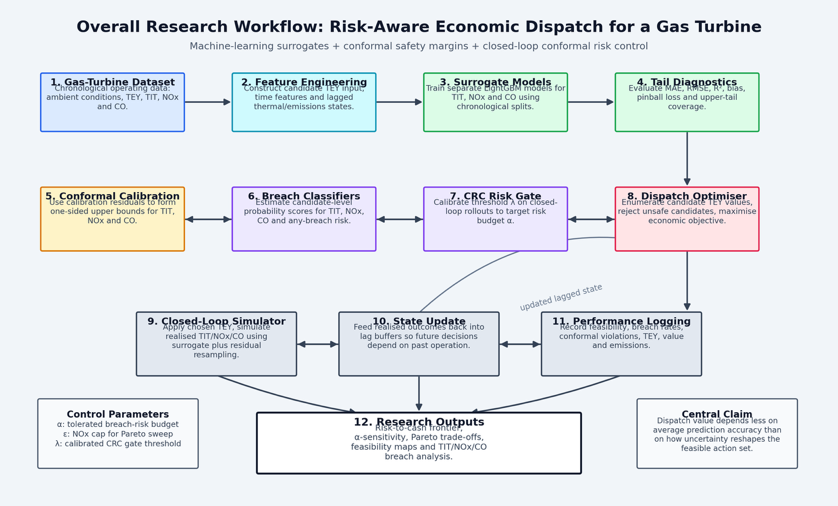
\includegraphics[width=3.76106in,height=2.27351in]{media/media/image2.png}}{}}\label{section-1}

\protect\phantomsection\label{_Toc228132494}{}Figure 1 - Overall
Research Workflow

\subsection{Context}\label{context}

Economic dispatch (ED) is an important problem in power systems. When
given demand and operating constraints, it allocates generator setpoints
to meet load while minimizing operating cost over a dispatch interval.
ED is usually posed with engineering constraints such as output limits,
ramping and operating envelopes, and re-solved as conditions change.
This is an elementary optimization task for reliable, efficient system
operation (Marouani et al., 2022).

Environmental constraints add more complexity to operational decision
making. Beyond fuel cost, operators often face requirements to limit
pollutant emissions, which motivates an approach that combines economics
and emissions in dispatch (CEED) that trade off operating cost against
emissions. This is commonly represented as a multi objective
optimization (Asif et al., 2024).

In this context, gas turbines are particularly relevant because their
emissions and thermal states vary strongly with operating points and
ambient conditions. The formulation of NOx is closely related to
combustion temperature and related thermos-chemical pathways. As such,
strategies that reduce peak temperature are important to NOx control in
turbines (Richards et al., n.d.). At the same time, CO emissions can be
restrictive at lower load operation where combustion completeness is
reduced, which creates an operational tension between flexibility,
thermal constrains and emissions (Lipperheide et al., 2018). These sort
of interactions between mechanisms means that operating points are not

automatically emissions safe, and that decisions during dispatch can
meaningfully change pollutant profiles.

Alongside this, there exists advanced predictive emissions monitoring
that estimate turbine emissions from routinely measured sensor and
ambient signals. Recent studies continue to develop data driven
emissions predictors for turbines using datasets (dos Santos Coelho et
al., 2024a). Together, ED/CEED formulations provides a system for
selecting setpoints under operational constraints, while gas turbine
emissions physics and data from monitoring can educated handling of
pollutant and thermal outcomes and quantities that are relevant for
decision making.

\subsection{Gap}\label{gap}

Dispatch research that is uncertainty aware usually considers risk
through chance constraints (the acceptability of constraints being
broken sometimes), stochastic optimization (where optimisation
explicitly considers randomness) or distributionally robust chance
constraints (DRCC, where you don't trust an assumed probability
distribution, so you optimise against a set of plausible distributions).
These approaches are good for providing probabilistic feasibility, but
they limited by their requirement for:

\begin{enumerate}
\def\labelenumi{(\Alph{enumi})}
\item
  An assumed certainty model
\item
  A scenario generation procedure
\end{enumerate}

(C) A specified ambiguity set (e.g. Wasserstein balls)

(Arrigo et al., 2022; Hu et al., 2017)

This presents a practical gap for settings where the plant is a learned
surrogate with not Gaussian (following a normal distribution),
heteroskedastic(the size/spread of errors change depending on the input
conditions), and regime dependent errors, and where operators need data
calibrated way to control risk, that changes depending on how the
turbine is operating.

Data driven modelling of gas turbine emissions is a rapidly growing
field, including studies that use the same UCI gas turbine CO and NOx
emission dataset mainly for benchmarked and methodological comparisons.
However, this area largely treats emissions modelling as an offline
prediction task. It rarely closes the loop by embedding predictors
inside dispatch decisions (Jhinaoui et al., n.d.), which quantifies how
error can propagate into operational constraint breaches, economic
outcomes, and feasibility failures over time. As a result, the
literature provides limited evidence on the quality of decisions and
safety when ML and NN surrogates are used in the optimizer.

Another foundation is distribution free uncertainty quantification.
Conformal prediction gives finite sample marginal guarantees under
exchangeability, and conformalised quantile regression improves
efficiency under heteroskedasticity -- which is the structure of error
you would expect to find in emissions/thermal variables in turbine
operating regimes. (Romano et al., n.d.). Conformal risk control further
generalizes conformal calibration to control expected monotone risks,
which suggests a pathway to calibrate risk threshold for `breach' events
rather than only prediction intervals (Angelopoulos et al., 2025). Time
series conformal methods such as EnbPl addresses sequential dependence
and nonstationary but are primarily presented in forecasting contexts
rather than in dispatch optimization (Xu and Xie, 2021). Conformal
methods have also begun to appear in safety critical control and MPC,
but these applications are usually outside of energy dispatch(Lindemann
et al., 2023a).

As such, this project targets an uncovered area that uses fast surrogate
models, enforced a calibrated safety margin, and reports risk
-\textgreater{} economy and NOx money frontiers under closed loop
simulation.

\section{}\label{section-2}

\subsection{Aims}\label{aims}

(A) Build a closed loop economic dispatch simulator for a gas turbine

(B) Train fast surrogate plant models

(C) Enforce Distribution free safety margins on emission variable and
CRC probabilistic risk gating by learning breach probability classifiers

(D) Quantify trade-offs for operators by producing
risk-\textgreater economy frontiers across a and e

\section{Background and Literature
Review}\label{background-and-literature-review}

\emph{This section defines the main components of the methodology, and
explains their context and implementation}

\subsection{Thermodynamic Foundation}\label{thermodynamic-foundation}

This section on the thermodynamic foundation explains why the variables
of interest (TIT, NOx, CO) coincide with thermal and emissions risk.
These are the same variables that also define the economic scope of the
project.

A gas turbine converts chemical fuel energy into shaft work through a
Brayton cycle (compression -\textgreater{} heat addition -\textgreater{}
expansion). The engineering reason a dispatch controller can control
energy output is that the net shaft work is an enthalpy balance across
the turbomachinery, while the internal temperatures and pressures that
determine work also governs material life limits, and the pollutant
formation kinetics (Ames Research Staff and Field, n.d.).

In compressible flow form, the enthalpy differential satisfies

\[\begin{array}{r}
dh = c_{p}dT\#(1)
\end{array}\]

And the inviscid adiabatic energy equation integrates into a constant
total enthalpy. This is the justification for writing component work in
terms of temperature changes (assuming that kinetic/potential changes
are small relative to enthalpy changes across compressor/turbine
stages). In a simple cycle using total stagnation temperatures, one may
write

\[\begin{array}{r}
w_{c} \approx c_{p},c\left( T_{t2} - \ T_{t1} \right),w_{t} \approx c_{p},t\left( T_{t3} - \ T_{t4} \right)\#(2)
\end{array}\]

So that the net specific work is

\[\begin{array}{r}
w_{net} \approx w_{t} - w_{c}.\#(3)
\end{array}\]

These are the thermodynamic reasonings for why energy yield (TEY)
behaves like a monotone function of firing temperature proxies and mass
flow. For a fixed dispatch hour, TEY is proportional to net power, and
net power scales with mass flow multiplied by net specific work.

For an ideal gas, the entropic differential and isentropic condition
yield the usual pressure-temperature laws. This is the formal
justification for expressing compressor and turbine outlet temperatures
as functions of inlet temperature, pressure ratio and component
efficiencies (Ames Research Staff and Field, n.d.).

These power law relations however rely on assumptions that become less
reliable in high temperature operation because \(c_{p}\)and \(\gamma\)
are not constants, and because modern turbines rely on bleeds and
cooling flows that disturb one-dimensional idealizations.

The following diagram details the relationships between gas turbine
behaviour and the targets:

\begin{figure}
\centering
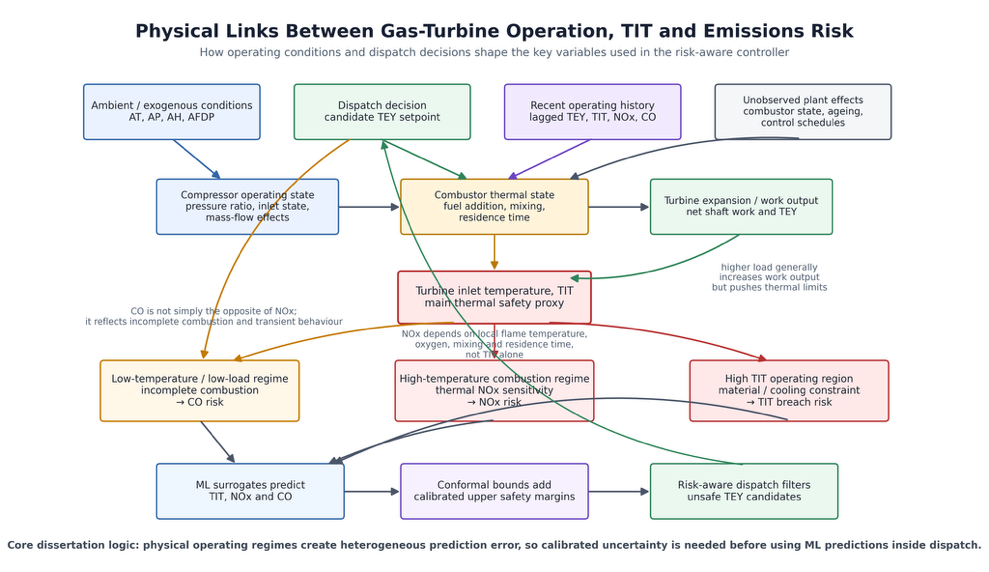
\includegraphics[width=4.47222in,height=2.39688in]{media/media/image3.png}
\caption{\protect\phantomsection\label{_Toc228132495}{}Figure 2 -
Physical Links between Gas Turbine operation, TIT, and Emissions risk}
\end{figure}

\subsection{TIT Decision Importance}\label{tit-decision-importance}

The operational rationale for using turbine inlet temperature (TIT) as a
main variable representing safety and economics is not just that higher
TIT gives more power. First order work sensitivity to TIT is large in
idealized balances. Under the constant \(c_{p}\) idealization, turbine
specific work is approximately

\[\begin{array}{r}
w_{t} \approx c_{p},t\left( T_{t3} - \ T_{t4} \right)\#(4)
\end{array}\]

Hence,

\[\begin{array}{r}
\frac{\partial w_{t}}{\partial T_{t3}} \approx c_{p,t}\#(5)
\end{array}\]

If \(T_{t4}\) weakly depends on \(T_{t3}\), even if \(T_{t4}\)
co-varies, a small \(\delta T_{t3}\) still maps into
order-\(c_{p}\delta T\) changes in work, so there is a strong dispatch
incentive to run near a temperature constraint.

However, that that sensitivity is not constant near high TIT, because at
elevated temperatures, \(c_{p}\) depends on temperature and gas
composition.

Modern thermochemical formulations represent \(c_{p}(T)\), h(T), and
s(T) via polynomial fits relative to reference thermochemical tables
(such as NASA polynomials and related coefficient sets; NIST-JANAF
tables) (Mcbride et al., 2002). As such, a more honest local sensitivity
is represented as

\[\begin{array}{r}
\frac{\partial w_{t}}{\partial T_{t3}} \approx c_{p},t\left( T_{t3} \right) + \left( T_{t3} - \ T_{t4} \right)dc_{p},\frac{t}{dT}\left. \  \right|_{T_{t3}} - c_{p},\frac{t\left( T_{t3} \right)\partial T_{t4}}{\partial T_{t3}}\#(6)
\end{array}\]

Which makes it explicit that \(c_{p}\) is a function not a constant, and
that the turbine exit temperature response matters. This is important
because the NACA compressible flow compilation separates perfect gas
relations from caloric imperfection corrections, because high
temperature applications require acknowledging variable property
behaviour(Ames Research Staff and Field, n.d.). Recent engineering
studies also show that flue-gas heat capacity depends on both
temperature and composition and can be correlated over wide temperature
ranges. This reinforces why a surrogate models' errors can be dependent
on regime and heteroskedastic near high load and high temperature
regions (Förtsch, 2025).

Industrial and aero gas turbines can reach high turbine inlet
temperatures because of advanced internal cooling of hot section
components, and thermal barrier coatings. Some reviews of rotating
component cooling describe cooling as essential for durability under
demanding temperatures and pressures and represent cooling as a major
engineering challenge (Unnikrishnan and Yang, 2022). On the materials
side, reviews emphasize that TBCs (thermal barrier coatings) operate in
demanding environments while identifying failure and degradation as
design constraints (Clarke and Levi, 2003).

This matters for learned surrogates because the dispatch optimizer wants
to buy power by pushing towards high TIT, but the feasible margin is set
by materials/cooling design realities. That creates a structurally high
value of risk calibration. The region that is most economically
attractive is near the boundary where predictive error has asymmetric
consequences (where a small underprediction can still cause a breach)
(Saravanamuttoo, 2017).

\subsection{Pollutant Formation Mechanisms and Temperature Sensitivity
for Nox and
CO}\label{pollutant-formation-mechanisms-and-temperature-sensitivity-for-nox-and-co}

\subsection{}\label{section-3}

It can be said mechanistically that many NO formation pathways in
combustion can be represented by temperature sensitive kinetics of
Arrhenius type:

\[\begin{array}{r}
k(T) = AT^{b}\exp\left( - \frac{E}{R\ T} \right)\#(7)
\end{array}\]

So that

\[\begin{array}{r}
\partial ln\frac{k}{\partial}T = \frac{b}{T} + \frac{E}{R\ T^{2}}\#(8)
\end{array}\]

When T is high and E (activation energy) is large, small \(\delta T\)
produces multiplicative changes in reaction rates (k) , inferring that
NOx often rises quickly with temperature in high load regimes
(Unnikrishnan and Yang, 2022).

It is important to note that TIT is not the same as peak flame
temperature, and NO formation depends on local temperature, oxygen
availability, mixing, and residence time. As such TIT ↑ ⇒ NOx ↑ is not
always valid. It is a proxy relationship whose slope and scatter are
dependent on the regime. Due to this, offline regression metrics can be
misleading. The highest impact errors are those that occur in the high
temperature tail where the kinetics make the system more sensitive
(Unnikrishnan and Yang, 2022).

CO emissions are tied to incomplete oxidation. CO tends to be elevated
when combustion is too cool, mixing is poor, or residence time is not
enough. That means CO is not redundant with NOx. NOx can be considered a
`hot pathway' risk, whereas CO is a risk factor for low temperature or
stability margin operation.

This asymmetry is one justification for treating CO and NOx jointly in
safety aware dispatch, rather than optimizing only one pollutant
(Pachauri, 2024).

An important implication here is that an optimizer that only penalizes
NOx my shift operation into regimes where CO or other stability
indicators may deteriorate. So multi-constraint feasibility is the more
defensible position for claims to do with `safe dispatch'.

\subsection{The Public Health}\label{the-public-health}

Modern power generating gas turbines emit NOx and CO as regulated
pollutants. These emissions vary strongly with load. NOx is emitted
primarily as nitric oxide (NO) and nitrogen dioxide (NO2). Once they are
released, NO2 and other particles in the NOx family interact with the
atmosphere in such a that forms ozone at the ground level and more
secondary particulate matter (nitrate aerosols). Both increase
respiratory and cardiovascular risk (United States Environmental
Protection Agency, 2025a). NO2 but itself is an airway irritant.
Exposure to it can aggravate asthma and respiratory disease. Long term
exposure is associated with susceptibility to respiratory infections
(United States Environmental Protection Agency, 2025a).

CO (carbon monoxide) is a toxic gas that binds to your haemoglobin and
can reduce the oxygen delivery to organs. As such, the primary health
concern for this pollutant is hypoxic stress for at risk individuals.
High exposure can be considered fatal (United States Environmental
Protection Agency, 2025b).

Environmental regulators set stack emission limit values and require
monitoring, because reducing stack concentrations reduces the chance of
exceedances after dispersion.

\subsection{}\label{section-4}

\subsection{Data Driven Gas Turbine Emissions
Modelling}\label{data-driven-gas-turbine-emissions-modelling}

An important question for data driven gas turbine emissions modelling is
whether surrogate models remain useful for decisions near operational
limits. Operational limits are where critical decisions would be mostly
made when managing risk. The UCI machine learning repository Gas Turbine
CO and NOx Emission Data Set (which is used in this methodology)
contains \textasciitilde36k hourly rows of sensor measures, including
TIT, TEY (MWh) and emissions (CO, NOx) in mg/m3. The samples are in
chronological order and recommends a specific time-based evaluation
protocol for `reproducibility and comparability' (UCI Machine Learning
Repository, 2019).

Recent studies using this dataset are usually organized around feature
engineering and model selection. They also report good point prediction
metrics. For example, a 2024 study evaluates multiple regressors, and
reports strong training performance but weaker validation performance,
which infers bad performance in generalization(dos Santos Coelho et al.,
2024b). Another 2024 paper shows improved RMSE vs baseline ML
regressors, and giving motivation for emissions monitoring for
compliance, in an offline context (Pachauri, 2024). A GPPS contribution
frames the task as multivariate time series regression and compares deep
learning architectures and feature-extraction approaches for CO/NOx
prediction (Jhinaoui et al., n.d.). A 2023 comparison argues that ML
outperforms physics-based models (Potts et al., 2023).

These papers collectively support a certain conclusion, that offline
predictive accuracy can be high, and modern approaches are competitive.

However, from a decision and control perspective, offline metrics are
not enough. Temporal dependence and shifts in regime means that random
splits can leak information and unreasonably increase confidence in
generalization, especially when the real deployment is sequential and
nonstationary. In addition, tail relevance must be considered.
Operations care about exceedances of limits (thermal, emissions). An
RMSE that looks good on average can still hide systematic
underprediction near the upper tail where constraints bind.
Compressible-flow and thermochemistry theory makes it clear that high
temperature conditions are where idealizations degrade and sensitivities
increase. As such, the data tails are an operationally dominant region
for safety.

Furthermore, once a predictor is embedded in an optimizer, the optimizer
will preferentially chose inputs that look good under the model. This
changes the realized distribution of operating points compared with the
training data. This can create systemic bias and invalidate naïve
calibration arguments unless they are accounted for specifically
(Perdomo et al., 2020).

As per what is seen in those papers, a more defensible evaluation would
combine:

(A) Contiguous time splits

(B) Regime conditioned evaluation as physics and error structure is
regime dependent

(C) Tail metrics targeted to exceedance risk rather than global RMSE
(Angelopoulos et al., 2025)

(D) Closed loop evaluation where model is assessed based on constraint
breaches, feasibility failures, and economic/emissions outcomes.

(Tibshirani et al., 2019).

\section{}\label{section-5}

\subsection{Optimizer-In-The-Loop
Approach}\label{optimizer-in-the-loop-approach}

In power system optimization, surveys of ML-assisted optimization show
that surrogate models can reduce computational burden and allow for
faster optimization loops, but they also show generalization and
reliability risks when operating conditions shift or when constraints
are evaluated under approximation (Tibshirani et al., 2019).

A conceptual difficulty, which is very relevant to dispatch, is that
optimization changes what is seen. When the optimizer uses a surrogate,
it chooses actions based on the learned structure from the surrogate,
which could potentially drive the system into regions where the
predictions are less reliable. This aligns with the concept of
performative prediction, which formalizes settings where prediction
influences outcomes and thusly shifts the data distribution. This effect
is an endogenous distribution shift (J. C. Perdomo et al., 2020). This
matters from the perspective of uncertainty calibration because
calibration guarantees rely on exchangeability (no points is
probabilistically special relative to one another) or stable sampling
(all new points are drawn under the same sampling rules as earlier
ones).

Conformal methods under covariate shift (a type of distribution shift
where the input distribution changes between training and deployment)
relaxes the requirement for exchangeability via weights when the
likelihood ratio can be estimated, which allows us to talk about
train-test input difference in a precise way (Tibshirani et al., 2019).
In optimization or design loops, the model helps choose which cases get
tested, so the real-world data depend on the model. This formalizes the
idea that that the optimizer tends to pick cases the model thinks looks
good (Xu and Xie, 2021).

When a dispatcher selects TEY setpoints based on predicted targets, the
realized residual distribution can be different from the calibration
residual distribution unless the simulation and calibration method
intentionally reproduces the optimized selection. The later talked about
implementation of simulated independent trajectories and calibrated
gating is a direct response to a known failure mode in ML + optimization
deployment.

\subsection{}\label{section-6}

\subsection{Distribution-Free Calibration and Risk
Control}\label{distribution-free-calibration-and-risk-control}

This project is concerned with imperfect and regime dependant surrogate
models where the optimiser can shift the operating distribution. Because
of this distribution free calibration and conformal risk control are
introduced as the mechanism for turning prediction uncertainty into a
usable safety margin.

Conformal prediction provides a way to take a models point predictions
and add an uncertainty range around them (conformal prediction). A
prediction interval such that over many future cases, the true value
falls inside the range about as often as promised by the definition
(marginal coverage). This is called distribution-free because the
guarantee does not require assuming a particular data distribution, but
it does however rely on the idea that past examples used for calibration
and the future examples that are predicted are drawn in the same way, so
their order can be changed without changing results (exchangeability).
All these reasons are why conformal prediction useful for calibrating
models, especially black box prediction engines.

For data that is time ordered, the assumption that `order doesn't
matter' fails because nearby time points are related. This temporal
dependence violates exchangeability. Methods such as EnbPl are designed
for this, where they produce uncertainty ranges step-by-step as new data
arrives using many refit models built from resampled data and
recalibrating using a moving window the most recent observations (Xu and
Xie, 2021).

Adaptive conformal inference (ACI) goes even further by adjusting
calibration online to maintain coverage under a shift of distribution
(Gibbs and Candès, 2021).

Theres a two-sided take-away here. Conformal tools are useful because
they are agnostic to the type of model used, and calibrated, but the
literature also shows that sequential dependence and distribution shift
requires adaptation to algorithms.

Conformal Risk Control (CRC) generalizes conformal calibration from
making prediction intervals that hit the true value most of the time.
Instead, it lets you set and guarantee a target level for how often a
chosen kind of bad outcome happens on average. It uses an error score
where larger mistakes count as worse. This makes it useful for
calibrating the chance of specific events.(Angelopoulos et al., 2025).

This is a good match for operational dispatch because many real
constraints are exactly in that form of exceedance events.

Conformal events ideas have been integrated into safety focused planning
by constructing uncertainty sets for predicted trajectories and
enforcing them in an optimization loop. A particular ``conformal MPC''
work argues that conformal prediction regions can be used to provide
probabilistic safety guarantees, when planning amid uncertain dynamics
(Lindemann et al., 2023b). More related work on conformal prediction
looks at how to update and report uncertainty in real time under
sequential data streams (Dixit et al., 2023).

For turbine dispatch, the value of this literature is less in copying
the specific formulations and more in the value of adopting the cautions
they prescribe. When the system's choices are influenced by the model,
the results can't be trusted by default, so you must design the process
carefully to avoid biased data caused by only looking at cases that pass
the chosen constraints.

\subsection{Multi-Objective Economic-Emissions Trade
Offs}\label{multi-objective-economic-emissions-trade-offs}

As the project studies economic dispatch under imperfect learned plant
models, the economic--emissions trade-off must be understood as a
frontier that is reshaped by uncertainty calibration, feasibility and
risk control.

The e constraint method generates `Pareto-efficient' solutions by
optimizing a primary object while turning other objectives into
constraints. It sweeps a parameter e to trace this frontier. Previous
works show that e-constraint has advantages over regular weighting
(which can miss parts of the frontier and is sensitive to scaling), but
also shows important issues, such as choosing e ranges, avoiding weakly
efficient points, and producing well distributed frontiers (Mavrotas,
2009).

In a dispatch setting where the primary objective is economic value and
the constrained objective is NOx, the formulation is

\[\begin{array}{r}
\max_{u \in \mathcal{U\ }}{J(u)}s.t.{\ \ \ E}_{(NOx)(u)} \leq \varepsilon,and\ operational\text{/}safety\ constraints\#(9)
\end{array}\]

This can be interpreted through the Lagrangian:

\[\begin{array}{r}
L(u,\lambda) = J(u) - \lambda\left( E_{\left( \text{NOx} \right)(u)} - \varepsilon \right)\#(10)
\end{array}\]

Where, at an efficient point, the variable
\(\left( \lambda^{*} \geq 0 \right)\) acts a local shadow price - shadow
price being the implied marginal value of relaxing/tightening the cap on
NOx. This provides a way to interpret economy/NOx slopes along the
frontier as marginal costs of NOx reduction (Mavrotas, 2009).

However critically, the MAC curve literature warns that marginal
abatement cost curves can be misleading if treated as uniquely
determined objects, because they depend on modelling assumptions and
interactions that can be hidden (Kesicki and Strachan, 2011). In this
context of this methodology, analogously it can be said that the
apparent `price' of NOx reduction depends not only on the optimizer
formulation, but also on the surrogate's calibration near the constraint
boundary and on feasibility filtering (conformal margins and breach
probability). Therefore, the frontier is a risk conditioned object that
is reported with breach and feasible hour fractions.

\section{Methodology}\label{methodology}

\section{}\label{section-7}

\subsection{\texorpdfstring{Problem Setup
}{Problem Setup }}\label{problem-setup}

An hourly dispatch problem over a time horizon is considered defined as

\[t = 1\ldots T\]

At each time t, the operator sets the turbine yield
\(u_{t\ }\  \geq 0\)MWh. The ambient exogenous variables (temperature,
pressure, humidity, filter pressure, etc.) and the previous operational
states \(u_{t - 1},\ TIT_{t - 1},\ NOx_{t - 1},\ CO_{t - 1}\), are
assumed known at time t. The surrogate then predict that at time t the
\(TIT_{t}\) and the emissions \(NOx(x,t),\ CO_{t}\) will be some
functions of \(\left( u_{t},AT_{t},AP_{t},AH_{t},AFDP_{t} \right)\) and
the lag past state.

Let

\[\widehat{Y_{t}} = f_{(point)}^{(Y)}\left( x_{t};w \right)\]

be the point prediction model for outcome
\(Y \in \left\{ ``TIT","NOx","CO" \right\},\ \)where \(x_{t}\ \)
collects the known inputs (including \(u_{t}\) and the lagged states) at
time t. W denotes the learned model parameters. An upper quantile model

\[f_{\tau}^{(Y)}\left( x_{t} \right)\]

Is also trained to estimate the \(\tau\)-quantile of Y, however the
online optimization constraints below are enforced using conformalised
upper bounds built from point prediction residual calibration. (See
Conformal Upper Bounds).

\subsubsection{Economic Objective}\label{economic-objective}

The economic objective at time t is set to maximize a net value function
defined as:

\[\begin{array}{r}
J_{t}\left( u_{t} \right) = \underset{(revenue)}{\overset{\left( Pu_{t} \right)}{︸}} - \underset{(fuel)}{\overset{\left( C_{(fuel)}\left( u_{t} \right) \right)}{︸}} - \underset{(wear)}{\overset{\left( C_{(wear)}\left( \overline{TIT_{t}} \right) \right)}{︸}} - \underset{(environment)}{\overset{\left( C_{(env)}\left( \overline{NOx_{t}},\overline{CO_{t}} \right) \right)}{︸}}.\#(11)
\end{array}\]

In the implementation, placeholder cost coefficients are used:

\[\begin{array}{r}
C_{(fuel)}\left( u_{t} \right) = 0.5u_{t},{\ C}_{(wear)}\left( \overline{TIT_{t}} \right) = 0.1\overline{TIT_{t}},C_{(env)}\left( \overline{NOx_{t}},\overline{CO_{t}} \right) = 0.2w_{(NOx)}\overline{NOx_{t}} + 0.05\overline{CO_{t}}\#(12)
\end{array}\]

With a fixed price P (P=10). The Nox weight is 1 by default and is
increased during \(\varepsilon\)-frontier sweeps to increase the
illustrative influence of Nox in the objective.

\subsubsection{Operational And Safety
Constraints}\label{operational-and-safety-constraints}

The control variable includes operational constraints. TEY is required
to be `feasible based on:

\[u_{t} \in \left\lbrack u_{\min},u_{\max} \right\rbrack\]

In the implementation \(u_{\min}\) is the 5\textsuperscript{th}
percentile of the training set of TEY, and \(u_{\max}\) is the
95\textsuperscript{th} percentile.

A fixed grid of candidate \(u_{t}\) values is used and solved via
enumeration.

Safety constraints are implemented using proxy limits. Let

\[\overline{TIT},\overline{NOx},\overline{CO}\]

be allowable upper limits on the targets. These are set as 95 percent of
the training data for each variable.

As predictions have error, these limits are enforced using calibrated
upper bounds. For each

For each \(Y \in \text{TIT},\text{NOx},\text{CO}\), we define a
conformal upper bound
\(\widehat{Y_{t}^{\left( \text{upper} \right)}}\left( u_{t} \right)\)
(see 3.1.3). The safety constraints are therefore:

\[\widehat{TIT_{t}^{(upper)}}\left( u_{t} \right) \leq \overline{TIT},\]

\[\widehat{NOx_{t}^{(upper)}}\left( u_{t} \right) \leq \overline{NOx},\]

\[\widehat{CO_{t}^{(upper)}}\left( u_{t} \right) \leq \overline{CO}.\]

A learned classifier for the probability of breaches occurring is used
as a `CRC gate'. For each candidate \(u_{t}\), breach probabilities are
calculated for every output, and an `any breach' score is calculated as:

\[\begin{array}{r}
s_{(any)}\left( u_{t} \right) = maxs_{(NOX)}\left( u_{t} \right),s_{(TIT)}\left( u_{t} \right),s_{(CO)}\left( u_{t} \right)\#(13)
\end{array}\]

A calibrated threshold \(\lambda(\alpha)\) is applied:

\[s_{\text{any}}\left( u_{t} \right) \leq \lambda(\alpha).\]

\subsubsection{Conformal Upper Bounds}\label{conformal-upper-bounds}

Recall that we define the point prediction as

\[\widehat{Y_{t}} = f_{(point)}^{(Y)}\left( x_{t} \right)\]

Calibration residuals \(r^{(Y)} = Y - \widehat{Y}\) are used; a
1-\(\alpha\) upper residual quantile is computed as \(q_{Y}(\alpha)\).
Therefore, in online usage, the calibrated upper bound is:

\[\begin{array}{r}
\widehat{Y_{t}^{\left( \text{upper} \right)}}\left( u_{t} \right) = \widehat{Y_{t}}\left( u_{t} \right) + q_{Y}(\alpha)\#(14)
\end{array}\]

This is applied separately for each target.

\subsubsection{Controller Optimizer Per
Hour}\label{controller-optimizer-per-hour}

Per hour t, the controller solves for

\[\begin{array}{r}
max_{\left( u_{t} \in \left( \mathcal{U} \right) \right)}{= J}_{t}\left( u_{t} \right)\#(15)
\end{array}\]

This is solved subject to all the predefined constraints.

Since U is a finite TEY candidate grid, this problem solved via
enumeration.

\subsubsection{Control Of Risk
Parameters}\label{control-of-risk-parameters}

Two main risk controls are used in this methodology.

The first is \(\alpha\) which controls miscoverage and risk level, where
miscoverage is the event that any stated guarantee fails, which is to
say the true value falls outside the predicted set. It is an array of
values used to decide the conformal residual quantities that define
\(Y_{t}^{\left( \text{upper} \right)}\), and it calibrates the CRC
threshold via conformal risk control so that the corrected expected
any-breach loss does not exceed \(\alpha\). This fixed grid of a is
defined in this set as {[}0.05, 0.07, 0.1, 0.15, 0.2{]}.

Secondly, we have \(\epsilon\) (the NOx cap). It is varied to trace a
--economics Pareto frontier. In these sweeps, one can increase the Nox
penalty weight so for the sake of clearer results or to align with
regulations, you can have a clearer Pareto separation between the
economic return and strictness of the constraints.

\subsection{Surrogate Model Training}\label{surrogate-model-training}

\subsubsection{Reasoning For Gradient Boosted Trees Over
NNs}\label{reasoning-for-gradient-boosted-trees-over-nns}

\paragraph{\texorpdfstring{What is LightGBM?
}{What is LightGBM? }}\label{what-is-lightgbm}

LightGBM (Light gradient boosting machine) Is a type of gradient
boosting decision tree (GBDT). It is a model that builds a set of
decision trees to minimize a loss. It is a supervised model (Ke et al.,
n.d.).

If given training data \(\left( x_{i},y_{i} \right)_{(i = 1)}^{n}\) and
loss \(\mathcal{l}\left( y,F(x) \right)\), gradient boosting creates a
predictor defined as:

\[\begin{array}{r}
F_{M}(x) = sum_{(m = 1)}^{M}\eta f_{m}(x)\#(16)
\end{array}\]

Where each \(f_{m}\) is a regression tree, and n is a learning rate. At
an iteration m, the algorithm uses gradients defined as:

\[\begin{array}{r}
g_{i} = \left( \partial l\left( y_{i},F\left( x_{i} \right) \right) \right)\text{/}\left( \partial F\left( x_{i} \right) \right)\left. \  \right|_{\left( F = F_{(m - 1)} \right)}\#(17)
\end{array}\]

This is the training signal used to choose splits that reduce loss the
most.

LightGBM evaluates a possible split by checking how well it separates
the data into left and right groups where the loss gradients are
strongest. It is computed from the sums of gradients in each child group
and selects the split with the largest gain.

\paragraph{Why Use Gradient Boosted Trees Over A Custom
MLP?}\label{why-use-gradient-boosted-trees-over-a-custom-mlp}

Gradient boosted decision trees (LightGBM in this implementation) is
used as the surrogate model because the problem is mostly tabular, mixed
scale data that requires fast retraining and iteration. Fast retraining
is important in an operator setting where the model is being updated
live with more data, and iteration is important in the development
environment. LightGBM is designed to train GBDT models efficiently
whilst retaining good accuracy. (Ke et al., n.d.).

Compared to neural networks, trees tend to have a stronger performance
on medium sized tabular datasets (such as the one used in this study)
without tuning. They are also less sensitive to feature scaling and
architecture choices. Studies show that tree based predictive methods
are very competitive and often perform better on tabular prediction,
before considering the cost of tuning NN models. (Grinsztajn et al.,
2022).

Since the methodology presented in this paper relies on surrogates that
can trained and validated quickly, LightGBM is an appropriate approach.

\subsubsection{Specific Surrogate Implementation
Used}\label{specific-surrogate-implementation-used}

\emph{The surrogate definition and setup can be found in Appendix B}

Separate surrogates are trained for the targets TIT, Nox and CO.

The data is assigned to a sequential array and sorted chronologically.

Masks are created via a split

\begin{itemize}
\item
  70\% train
\item
  15\% calibration
\item
  15\% test
\end{itemize}

These splits are in earliest -- latest order.

For each hour t, the feature vector includes

\[x_{t} = \left\lbrack AT_{t},AP_{t},AH_{t},AFDP_{t},u_{t},\text{time features},\text{lagged state features} \right\rbrack\]

Where \(u_{t}\) corresponds to TEY (the dispatch decision).

Notice not all features of the original dataset are included to prevent
leakage. This is further explored in Failure Modes.

For each target Y, two LightGBM regressors are trained. The first is the
point model

\[\widehat{Y_{t}} = f_{(point)}^{(Y)}\left( x_{t} \right)\]

And the upper quantile model (later used for the CQR bounds and
evaluation)

\[\widehat{q_{t}} = f_{\tau}^{(Y)}\left( x_{t} \right),\ \ \tau = 0.95\]

Both models use the same core hyperparameters defined in appendix B.

In terms of evaluation, for point models, MAE and \(R^{2}\)are computed
on TRAIN / CALIBRATION / TEST split.

For quantile models, pinball loss and empirical coverage
\(\Pr(Y \leq \widehat{q})\)are computed on TRAIN / CALIBRATION / TEST
(nominal target \(\approx \tau\)).

Calibration residuals from the point model on the CALIBRATION split are
saved for downstream conformal upper bounds, and CQR scores based on
\(Y - \widehat{q}\) are computed.

\paragraph{Hyperparameter tuning and
justification}\label{hyperparameter-tuning-and-justification}

\emph{Hyperparameter choices for the surrogates can be found in appendix
B}

The surrogate hyperparameters were chosen to be conservative and
reliable rather than aggressively tuned for pure accuracy. There is a
low learning rate, high tree a cap and early stopping that provides
stable fitting. The row and feature subsampling regularise the model and
the tau = 0.95 matches the safety role of the upper tail model. The
settings were chosen to enable fast retraining in testing, with decent
generalisation. These provided satisfactory results.

\subsubsection{\texorpdfstring{Lags And Their Physical Significance in
Emission Prediction
}{Lags And Their Physical Significance in Emission Prediction }}\label{lags-and-their-physical-significance-in-emission-prediction}

Lag features are created that hold 3 previous hours of any given
feature/target.

To avoid leakage and retain a desirable signal, all the targets use the
baseline exogenous features, plus the time features, plus a baseline
single hour lag feature:

\[TEY_{(t - 1)},TIT_{(t - 1)},GTEP_{(t - 1)},TAT_{(t - 1)},CDP_{(t - 1)}\]

Rows are dropped until all the required lagged features are available to
the model.

The NOx and CO model additional includes lag states 1-3 to improve
prediction accuracy. Gas turbine emissions have memory. During load
changes and variation in ambient conditions, the internal states relax
over time so the conditions at any given moment depend on the recent
operating history. This is due to effects like heat transfer and soaking
that define future performance (Yang et al., 2024). In this dataset,
each row is an hourly aggregate, so a single hour can mix steady periods
and transients; lags help the surrogate infer whether hour t follows a
ramp-up, ramp-down, or settled regime, improving accuracy especially
near constraint boundaries.

Initial prediction accuracies were very challenging before lags were
introduced, proving that transient information is essential to correctly
prediction these emissions.

\subsection{Conformal Calibration}\label{conformal-calibration}

For each of the outputs TIT, NOx and CO, the controller requires an
upper (one sided) safety margin that can be calculated cheaply for every
setpoint. As such, a split conformal upper bound is implemented as a
residual translation of the point surrogate. The single predictions are
taken, and then a safety margin is added based on the past prediction
errors. This is the standard implementation for one-sided conformal
prediction of this form (Fontana et al., 2023),

After training each point surrogate, the residuals are computed not on
the training set, but the calibration set

\[r_{i}^{Y} = y_{i}^{Y} - {\widehat{y}}_{i}^{Y},\ \ i = 1,\ldots,n_{cal}.\]

We also let

\[r_{(1)}^{Y} \leq \ldots \leq r_{\left( n_{cal} \right)}^{Y}\]

be the sorted set of residuals. The conformal slack (safety margin added
to the point prediction so the resulting bound achieves the target
coverage) is computed using the finite-sample order statistic index:

\(k = \left\lceil \left( n_{cal} + 1 \right)(1 - \alpha) \right\rceil\)
\(\begin{array}{r}
 = r_{(k)}^{Y}\#(18)
\end{array}\)

(Shafer and Vovk, 2008)

Given a vector x that defines the candidate feature set, including the
TEY setpoint, the per target conformal upper bound is

\[\begin{array}{r}
{\widehat{U}}_{Y}(x;\alpha) = {\widehat{y}}^{(Y)}(x) + {\widehat{q}}_{Y}(\alpha)\#(19)
\end{array}\]

This choice can be justified due to the fact the one sidedness
concentrates the calibration on the relevant tail, and the translation
form keeps the safety evaluation constant-time and stable across the
candidate TEYs, which is important as it calculates many candidates per
operation hour.

Because predictions errors for the emissions and temperature are likely
heteroskedastic across operation, an upper quantile model at the
95\textsuperscript{th} percentile is also fit. The n a conformal
quantile regression (CQR) is fitted on the calibration data using the
usual conformal score values (these are based on how far observations
fall above the predicted quantile) for diagnostics.

Operating under the assumption that the calibration data and future test
points are exchangeable (exchangeability), the one sided conformal upper
bound has a finite sample marginal guarantee defined as:

\[\begin{array}{r}
\Pr\left( Y \leq {\widehat{U}}_{Y}(X;\alpha) \right) \geq 1 - \alpha\#(20)
\end{array}\]

Which is essentially saying for any given target Y, the true value will
be below the upper bound at least 1-\(\alpha\) times, and this holds
separately for each target.

Since the TIT, NOx and CO limits are enforced at the same time, a good
performance on each limit by itself does not guarantee that the chance
of violating at least one limit is controlled. To be clear, even if each
constraint rarely fails or is infeasible when checked individually the
probability that one or more constraints can still be higher.

The implementation logs, for every decision three separate decisions.
Was TIT violated, was NOx violated, and was CO violated? It then has one
combined log, was ANY constraint violated? This is true of any of the
three flags are true.

It logs both the per constraint violation rates and the overall,
any-violation rate.

\subsection{CRC Threshold}\label{crc-threshold}

The conformal upper bounds control the model error on each prediction,
but they don't directly control the decision induced frequency of
breaches of said constraints once the operator makes its decision. This
is considered endogenous distribution shift as the resultant change in
data distribution is caused by the model or decision system itself. This
mechanism is formalized in performative prediction, where decisions
taken using a model can change the distribution of the outcomes (J.
Perdomo et al., 2020).

As such, the implementation adds a separate gating layer of which's
purpose is to control an operator specified risk variable a on a loss
function measures whether and by how much a quantity exceeds the
specified limit. It can therefore be said that for each constraint
variable, a binary breach label is defined on the training split using
the same proxy limits used by the dispatch constraints

\[\begin{array}{r}
B^{(Y)} = 1\left\{ Y > \overline{Y} \right\}\#(21)
\end{array}\]

This is implemented by computing the proxy limits from the train data,
and training three LightGBM classifiers to predict \(B^{Y}\) from the
same feature et used by the surrogates.

At runtime these classifiers produce scores per candidate hour

\[\begin{array}{r}
s^{(Y)}(x,u) \in \lbrack 0,1\rbrack\#(22)
\end{array}\]

The gate combines them into the any-breach score used to filter the
candidate TEY actions before maximization for the objective.

It is important to note that this method does not require the classifier
probabilities to be calibrated. A benefit of conformal risk control is
that it only needs a scalar score that is subject to a threshold,
because the threshold itself is calibrated distribution free.

The cutoff gate λ (\(\alpha\)) is not chosen heuristically. It learns
the cutoff from using data from the CRC calibration step where each data
point is a whole simulated run of the controller, rather than a single
sample. This choice is significant for multiple reasons. The cutoff λ
(\(\alpha\)) changes which candidate actions are allowed, which changes
the actions the controller takes, which changes which states the system
visit*, which in turn changes the observed rate of constraint breaches.

As such, the breach statistics that the operator cares about depends on
the gate itself. Calibrating the λ (\(\alpha\)) on the closed loop
trajectories make the calibration data reflect the same distribution
that will be seen at deployment.

In other words, the calibration is done with the controller within the
loop, rather than calibrating on a fixed open loop score that ignores
how the method alters what is observed.

A larger λ(\(\alpha\)) should increase the allowed hours and therefore
increase risk. However, since the risk is found from a finite number of
trajectories, Monte Carlo noise can make the measured loss sometimes
reduce at higher λ. To fix this, the monotonizes the loss curve over the
λ gride by taking a cumulative maximum. At each λ the reported loss is
replaced by the largest loss seen at any small λ.

This stabilizes the calibration and enforces the monotone loss condition
that is required by conformal risk control.

If we let \(\widehat{R}(\lambda)\) be the mean trajectory loss over the
trajectories, then it can be said the correction is defined as

\[\begin{array}{r}
{\widehat{R}}_{(corr)}(\lambda) = \frac{1 + \widehat{n}\left\{ R \right\}(\lambda)}{n + 1}\#(23)
\end{array}\]

This correction is standard in conformal risk control guarantees for
bounded monotone losses under exchangeability (Angelopoulos et al.,
2025).

*'The states the system visits' means the sequence of actual operating
conditions the system passes through over time

The following diagram displays a flow chart of the dispatch hierarchy:

\begin{figure}
\centering
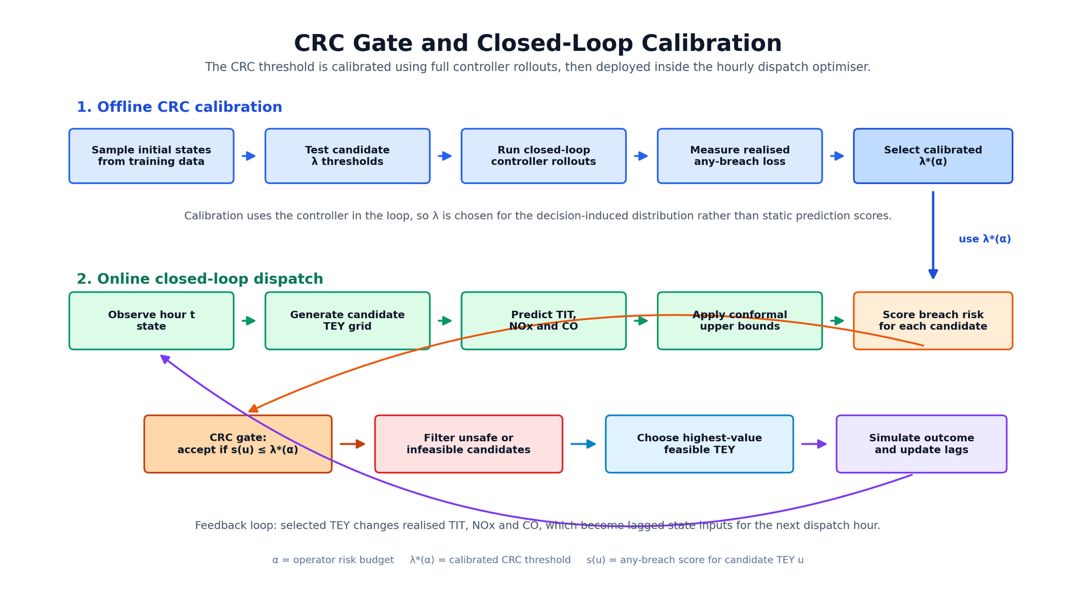
\includegraphics[width=4.84259in,height=2.74724in]{media/media/image4.png}
\caption{\protect\phantomsection\label{_Toc228132496}{}Figure 3 - CRC
and Closed Loop Calibration}
\end{figure}

\subsection{Closed Loop Simulator}\label{closed-loop-simulator}

To measure how well the controller performs under feedback (when its own
decisions affects future hours), it is tested in a closed-loop
simulation in a receding horizon. Each hour, the controller uses the
latest state, solves the constrained optimization again, applies the
optimised action, and then moves onto the next state.

This is consistent with standard model predictive control methods. (J.
Perdomo et al., 2020)

The simulator separates the exogenous inputs from the endogenous state
that evolves under the controller's decisions.

In terms of inputs, for each simulated how t, the ambient and other
non-controlled signals are (ATt\hspace{0pt}, APt\hspace{0pt},
AHt\hspace{0pt}, AFDPt\hspace{0pt}), and a time index hour are taken
from the dataset for that hour. These are immutable, observed, and
uninfluenced by the controller.

Here we define a term `policy'. The policy means the rule/s the
controller uses to choose the next action from the current information
that is available to it. Consider the policy just the set of rules
describing each decision.

The policy's information state is represented by a stack of lagged
process variables, which are advanced deterministically each step. The
controller has a dense history buffer per state variable, but it only
passes the selected past values exactly needed by the optimizer in the
optimization step. This makes sure that the lagged features correctly
propagate under all conditions.

When rolling out the simulator under the test set, the code should
initialise to the lagged state using the final row from the calibration
period, which gives the first test time steps realistic recent history
instead of starting with empty or artificial past values. When running
the CRC calibration rollout, the initial state is instead taken by
sampling a starting row from the training data. This is because a lagged
model cannot make a realistic prediction at the first simulated hour
unless it knows the recent past, and seeding in this way allows for
plausible operation.

\textbf{Inner Loop}

At each hour, the simulator constructs a candidate set of actions

\[u\mathbf{\in}U\]

as an evenly spaced grid between the 5\textsuperscript{th} and
95\textsuperscript{th} percentile (to avoid extreme extrapolation) of
the training set of TEY.

For each possible action, the implementation checks whether it satisfies
the TIT/NOx/ CO upper bound limits, the CRC risk gate, and extra NOx cap
rule for better pareto results. Only actions that pass all active checks
are allowed. If no action passes, that time step is marked infeasible,
and the code records which constraint blocked the most candidates.

To close the loop, the simulator needs a model of realized outcomes
after applying the chosen action.

The implementation uses a nonparametric residual resampling model
defined as:

\[\begin{array}{r}
Y_{t}^{\text{sim}} = \widehat{Y_{t}}\left( u_{t} \right) + \widetilde{r_{Y}}\#(24)
\end{array}\]

\[\widetilde{r_{Y}} \sim \text{Unif\{}r_{i}^{(Y)}\text{\}}_{i \in \text{CALIB}}\]

This is applied independently for
\(Y\mathbf{\in \{}TIT\mathbf{,}NOX\mathbf{,}CO\}\), where the
calibration residuals are computed on the calibration split and stored
as arrays for sampling later.

The simulation creates outcomes in two parts. One is the surrogate where
it's the model's prediction for what should happen after an action, and
one is the empirical disturbance, which is a randomly sampled past
prediction error taken from the calibration residuals. This means that
instead of assuming a fixed noise model, the code uses the actual error
patterns seen in past data, defining the `distribution free' requirement
earlier discussed.

This can be compared to a residual bootstrap, where error is
approximated by past data rather than a parametric form, allowed you to
test the controller in a difficult but realistic setting where the
optimiser keeps choosing actions close to the defined limits. These
boundary cases are where the calibration and gating matter the most
because small prediction errors can decide whether a constraint is
satisfied or violated.

(Efron, 1979; Freedman, 1981).

After the simulator generates the actual outcome for the current hour,
it updates the systems memory of recent past values by moving each
history buffer forward by one step and adding the newest realized values
for the targets and TEY. For unused unmodeled lagged variables it just
copies the observed value from the matching row in the dataset when
updating for the new state.

At each hour the simulator records 4 things:

\begin{enumerate}
\def\labelenumi{\arabic{enumi})}
\item
  The chosen action and data surrounding it
\item
  The simulated realized outputs and whether breaches occurred
\item
  Conformal audit flags which mark whether the realized value was above
  those hours calibrated upper bound
\item
  Per hour Feasibility data
\end{enumerate}

This logging is important because conformal calibration is only
meaningful in terms of what ends up occurring during operation. (Lei et
al., n.d.).

\begin{figure}
\centering
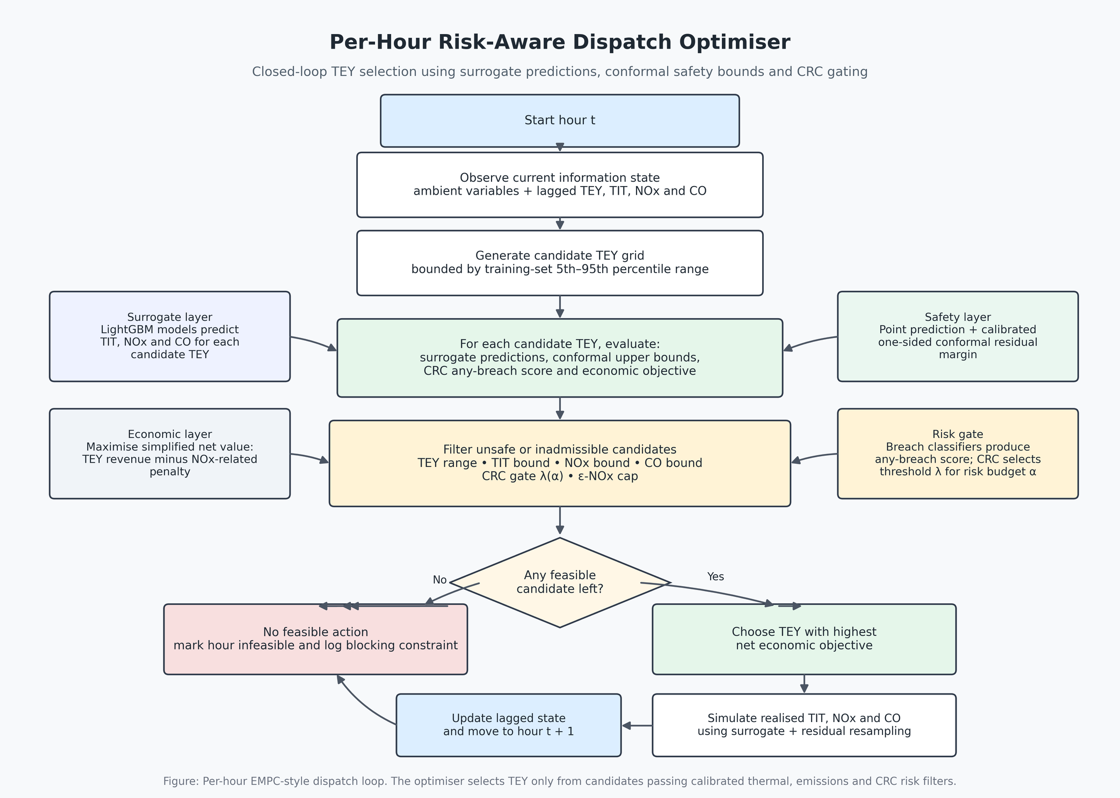
\includegraphics[width=5.05556in,height=3.46307in]{media/media/image5.png}
\caption{\protect\phantomsection\label{_Toc228132497}{}Figure 4 - Per
hour dispatch optimiser}
\end{figure}

\subsection{Assumptions, Limitations,
Complexity}\label{assumptions-limitations-complexity}

\subsection{}\label{section-8}

\subsubsection{Assumptions}\label{assumptions}

The controller implementation does not assume full plant stationarity,
meaning that the plants underlying behaviour is not assumed to be stable
in the time domain. It does however assume that the chosen lagged state
representation is sufficiently informative for accurate approximation at
the scale. Aspects like slow thermal memory, actuator hysteresis, the
state of maintenance and other plant effects are all absorbed into the
residual error.

A second assumption is the transferability of calibration. The conformal
upper bounds and CRC are calibrated and reused in the closed loop
simulation, which in effect assumes that the uncertainty that is faced
during deployment is similar enough to the uncertainty seen in
calibration. This assumption wants the logic to remain informative
through these splits. This assumption is however justified because
conformal prediction gives marginal validity under exchangeability, and
CRC extends the same calibration logic to monotone risks. However, with
turbine data, that interpretation becomes approximate rather than exact,
since exchangeability can be violated by non-stationarity. (Lei et al.,
n.d.)(Angelopoulos and Bates, 2022)(Xu and Xie, 2021).

Thirdly, the methodology assumes that safety can be totally captured by
exceedance events, rather than knowing the full probability distribution
of outputs. This makes sense for operators because they directly care
about whether temperature or emissions limits are breached, however the
code only can control that event-based risk. It cannot provide a
probabilistic calibration of the outputs and thus cannot make claims
that have equally strong validity in every operating condition. (Foygel
Barber et al., 2021).

\subsubsection{Limitations}\label{limitations}

The controller picks TEY setpoints based on what the surrogate predicts
will look best. Because of that, it will keep choosing operating
conditions that the model rates as attractive and will spend less time
in other parts of the operating range. As a result of this, the data the
plant produces after deployment may no longer look like the data used to
train and calibrate the model. The train-calibrate-test and closed loop
setup help because they test the method in a more realistic way than
checking one step prediction accuracy offline, but it still doesn't
completely solve the problem. Once the model starts influencing which
actions are taken, it also starts influencing which data gets observed,
so the real-world data distribution can shift because of the model
itself. This is a core tenet of performative prediction theory. (J. C.
Perdomo et al., 2020).

\subsubsection{}\label{section-9}

Related to this the uncertainty guarantees apply mainly in a average
sense, not for every specific operating condition. SO even if the method
controls breach well on average, it can still be less reliable in rare
or poorly represented parts of the operating range, such as in unusual
weather conditions or extreme temperature cases.

Another limit is that the methodology is limited in its external
validity. It is trained and evaluated on a single public gas-turbine,
uses proxy caps, and has illustrative economic coefficients. In
addition, the dispatch omits several operational constraints that matter
in practice like ramping, start up and shut down logic, variation in
fuel types and quality, aging of components etc. Such a design is
suitable for a methodological demonstration, but broad and defensible
claims for deployment outside of this sample are unjustifiable without
more external validation, additional plants or time splits. (Collins et
al., 2024)

There is a limitation based on the structural modelling of the
methodology. This is based on the choice to use separate target wise
surrogates and breach models. This allows training and inference to be
fast and modular, but it also means that dependence between targets is
only handled indirectly through the `any-breach' gate and the shared
features. This is a more pragmatic approach to protect against
exceedance, rather than using a more explicit, multivariate and
stochastic model of the targets.

The controller works via grids and a one-step greedy search. As such, it
inherits the limitations imposed by them. Enumerating a fixed grid makes
the dispatch logic robust, but it can miss better hours depending on the
grid size and it doesn't optimise over long intertemporal horizons
(meaning the span of future time periods over which decisions are
planned and linked together). As such, the frontiers seen is results
should be understood as showing the trade-offs achieved by the specific
one step and update control policy, rather than the best possible trade
offs for the economics and pollutants.

\subsubsection{Computational Complexity}\label{computational-complexity}

\paragraph{Current Offline Implementation
Complexity}\label{current-offline-implementation-complexity}

\emph{For this section the nomenclature can be found in appendix C1}

Gradient Boosted trees are a histogram based boosting method, so a proxy
for the order of training is linear in sample size, feature count, and
boosting rounds (Ke et al., n.d.).

\[\begin{array}{r}
C_{it} = \sum_{t = 1}^{P}{O\left( N_{tr}d_{t}\left( M_{t}^{pt} + M_{t}^{gu} + M_{t}^{br} \right) \right)}\#(25)
\end{array}\]

The conformal stage is cheaper than fitting the model, but in the
implementation, it is repeated over all the risk levels and uses
sorting-based quantile extraction on the calibration residuals. This
yields:

\[C_{\text{conf}} = O\left( PAN_{\text{cal}}\log N_{\text{cal}} \right)\]

In here CRC isn't just used in the thresholding, it also relies on the
extra breach classifiers defined above, and then it calibrates a
threshold by the simulated rollouts. The theory states that it expects a
loss up to the O(1/n) term, but the implementation cost is instead
driven by the amount of simulated trajectories and candidates for the
thresholds.

If we let \(c_{cand}\) be the cost of evaluating all the fitted models,
each dispatch step enumerates a TEY grid, predicts the targets and
breach probabilities for all candidates, and applies the conformal and
CRC feasibility masks, and picks the best economic objective. As such:

\[C_{\text{hour}} = O\left( G_{\text{cand}} \right)\]

Over T hours, the baseline frontier costs
\(O\left( ATG_{\text{cand}} \right)\). CRC calibration costs

\[C_{\text{CRC}} = O\left( ALRHG_{\text{cand}} \right)\]

And the e-constraint sweep adds a factor of

\[C\varepsilon = O\left( AETGc_{cand} \right)\]

Therefore, the complexity could be defined as:

\[\begin{array}{r}
C_{\text{offline}} = C_{\text{fit}} + O\left( PAN_{\text{cal}}\log N_{\text{cal}} \right) + O\left( ALRHG_{\text{cand}} \right) + O\left( ATG_{\text{cand}} \right) + O\left( AETG_{\text{cand}} \right)\#(26)
\end{array}\]

\paragraph{If new data were added sequentially in a live
system}\label{if-new-data-were-added-sequentially-in-a-live-system}

The current implementation does not have live streaming updates. If a
new hour were added and the saved models, conformal summaries and CRC
thresholds were kept, then it would still cost:

\[C_{\text{live/hour}} = O\left( G_{\text{cand}} \right)\]

If, however, the same batch pipeline was rerun whenever new data
arrived, then after t arrivals with Nt = N0 + t,

\[\begin{array}{r}
C_{\text{refit}}(t) \approx \sum_{j = 1}^{P}{O\left( N_{t}d_{j}\left( M_{j}^{pt} + M_{j}^{gu} + M_{j}^{br} \right) \right)}\#(27)
\end{array}\]

Repeating that after every new arrival of data gives a cumulative cost
that grows about quadratically in the live situation. Thus, for a live
implementation, computation becomes expensive unless the offline
artifacts are fixed or refreshed infrequently.

\subsection{\texorpdfstring{Issues encountered
}{Issues encountered }}\label{issues-encountered}

\subsubsection{\texorpdfstring{Low model accuracy without considering
time dynamics
}{Low model accuracy without considering time dynamics }}\label{low-model-accuracy-without-considering-time-dynamics}

\emph{All results for this section can be found in appendix B7}

Initially the system was modelled in the surrogate without lagged
features. That design as acceptable for TIT, but it performed badly for
the emissions targets. On the test split, the no-lag model gave TIT MAE
= 3.08, RMSE = 4.04, and R² = 0.956, but NOx deteriorated badly to MAE =
12.20, RMSE = 14.07, and R² = -1.82, while CO only reached MAE = 0.791,
RMSE = 1.36, and R² = 0.535.

The tail diagnostics showed the same issue, where the NOx test pinball
was 1.040 and CO empirical coverage was only 0.749. This is an indicator
weak upper tail reliability, which is perhaps the most important aspect
for the projects constraint logic.

I realised this was a modelling problem rather than a hyperparameter
tuning problem. In this dataset, each observation uses chronological
splits, so the current row can still reflect recent thermal relaxation,
and incomplete settling from previous hours. Gas-turbine transient
studies also show that load changes and ambient variation shift the
system away from thermal equilibrium, while emissions depend on
combustion temperature, time, and related internal states rather than on
just instantaneous inputs. This is to say, NOx and CO are partly
state-dependent and therefore need recent operating history to be
inferred properly (As discussed in the Lag section).

I therefore added lagged state features, with three previous hours
included for the emissions models. After doing so, the final test
results improved materially.

TIT improved to MAE = 2.15, RMSE = 2.94, and R² = 0.976. The largest
gain was in NOx, which improved to MAE = 3.91, RMSE = 5.13, and R² =
0.625. CO also improved to MAE = 0.456, RMSE = 1.04, and R² = 0.731. The
tail metrics improved as well: NOx pinball fell to 0.482, CO pinball to
0.105, and CO empirical coverage rose to 0.854.

This supports the interpretation that lagged features restored missing
dynamic state, which was especially important for NOx and CO because
their values depend more strongly on recent combustion history than TIT
does.

\subsubsection{Unfaithful CRC
implementation}\label{unfaithful-crc-implementation}

In initial approaches to completing the CRC implementation, an
approximated version of CRC logic was implemented. The old approximation
worked by after training the breach classifiers for the targets, it then
chose three separate cutoffs by taking upper quantiles of the
calibration scores themselves. The optimiser accepted an action only if
all three scores were below their own thresholds. That is a reasonable
heuristic gate, but it is not the idea that CRC guarantees. CRC does not
guarantee validity for arbitrary score quantiles. It guarantees control
of the expected value of a bounded monotone loss after calibrating the
control parameter on held-out data with the CRC correction.(Angelopoulos
and Bates, 2022).

The problem is that the first method calibrated in open loop. It looked
only at fixed calibration scores. It did not measure the realised breach
loss after the controller had filtered actions and changed the state
sequence. In a control setting, that distinction is very important.
Decisions change which states are visited and therefore change the
breach distribution, therefore, a threshold that looks right on static
calibration scores is not, by itself, a CRC guarantee for the deployed
controller. It also controlled three marginal score tails, not the
deployed any-breach risk that the dissertation claims to bound.

The revised implementation matches the CRC template much more
accurately. The improved implementation first forms a single any-breach
score, then builds a candidate λ grid from calibration scores. For each
λ, it runs full closed-loop EMPC rollouts on independent sampled
trajectories, computes a realised any-breach loss, enforces monotonicity
of that loss curve, and applies the finite-sample CRC correction
\((1 + n*risk)\text{/}(n + 1)\)before selecting the largest admissible
λ.

Let us compare these images of the old and new implementation.

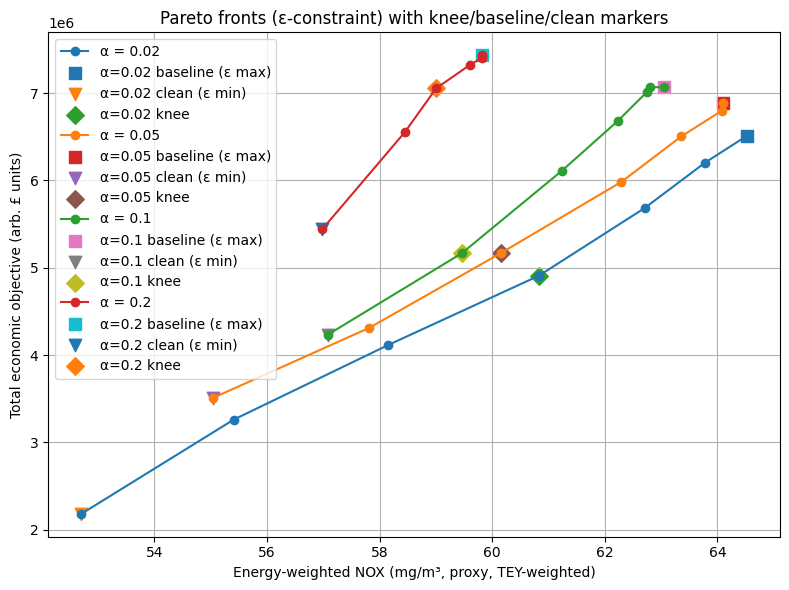
\includegraphics[width=2.81946in,height=2.10465in,alt={A graph with different colored lines AI-generated content may be incorrect.}]{media/media/image6.png}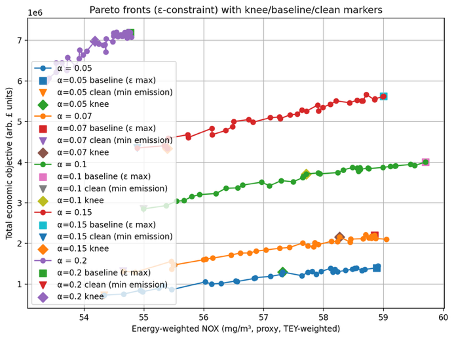
\includegraphics[width=2.69048in,height=2.01489in,alt={A graph of different colored lines AI-generated content may be incorrect.}]{media/media/image7.png}

\protect\phantomsection\label{_Toc228132498}{}Figure 5 - Old CRC
Implementation

\protect\phantomsection\label{_Toc228132499}{}Figure 6 - Improved CRC
implementation

On the left (old implementation) we see the distribution frontiers are
more overlapped, and sometimes hard to interpret as a clean hierarchy of
risk. Higher risk settings can look too strong, and some curves partly
dominate lower-α curve.

For example. The 0.2 frontier has a high economic value without a
proportionate NOx penalty. In the improved implementation, the frontiers
are more distinctly ordered by α. Lower α now clearly gives lower money
and lower NOX. Higher α clearly buys back value. The whole family of
curves is also shifted leftward in NOX space, especially at higher α,
and the low-α frontiers are much more punitive in economic terms. The
new implementation makes α correspond much more directly to the actual
safety object the operators care about, which is an important tenet of
this methodology.

\subsubsection{Computation time}\label{computation-time}

\subsubsection{}\label{section-10}

During development of the implementation, the high number of nested
loops resulted in extensive runtimes per test if the models. This is due
to the repeated closed loop simulations for every trajectory of the
optimiser. This slows down debugging and testing as it reduces the rate
at which results can be iterated. To solve this, a separate workflow was
implemented defined as a fast development mode vs a final run. The code
has explicit runtime controls through a separate set of variables that
reduced many variables like the simulation set, TEY and LAMBDA grid
size, and the number of trajectories. This means for the same data and
the same saved surrogate artifacts, a lower resolution full result set
can be run.

Another optimisation was reducing the need to rerun expensive steps that
didn't require rerunning to get results. Surrogate training and
rebuilding the dataset features was implemented in a separate runtime
and saved to hardware, such that they only needed to be run when changes
had to be made for those specific features. This modularisation also had
significant positive effects on computation time and general efficiency
of development.

\section{Results And Discussion}\label{results-and-discussion}

\section{}\label{section-11}

\subsection{Description of Result Set}\label{description-of-result-set}

The results are presented in two parts. Initially it's the surrogate
training report. For each target, the exported results include the point
model metrics by split, and quantile model metrics by split, with a
conformal coverage profile across a and CRC classifier summary.

Second, the EMPC + CRC simulation produces a set of results over the
risk array:

\[\alpha\mathbf{\in}0.05\mathbf{,}0.07\mathbf{,}0.10\mathbf{,}0.15\mathbf{,}0.20\]

The main risk-to-cash table records, for each α, total MWh, total
economic objective, feasible and infeasible hours, feasible fraction,
mean and standard deviation of TEY, realised per-pollutant breach rates,
realised any-breach rate, and conformal violation rates. A separate
e-constraint Pareto table reports, across α and NOX-cap values, mean
simulated NOX, feasible-only NOX, economic objective, risk metrics, and
feasibility metrics.

\subsection{Key Result}\label{key-result}

Across the experiments, the main result is the idea that small changes
in the risk gate can produce large changes in the existence and size of
a feasible action set. In control terms, feasibility is a proxy for
whether a dispatch algorithm can reliably keep the plant in an allowable
envelope given model error. The practical implication is that, for
ML-in-the-loop dispatch, the unit of analysis should be how error
reshapes the feasible set and therefore the policy.

There is a clear general trend that more risk allowance results in
higher economic objective, subject to certain modelling nuances. The
results imply that with the available sensors on the test case, one
pollutant is structurally harder to learn, and another is structurally
harder to bound in the tails of its characteristic data. As previously
described, NOx is strongly shaped by flame temperature, mixing,
residence time, and control schedules that are not directly represented
in the UCI sensor set. As a result, two hours with similar ambient
conditions and TEY can correspond to different internal combustor
states, so the mapping from available features to NOx is inherently
noisy from the model's perspective. CO is generally linked with
transient operability constraints. These regimes often create
heavy-tailed behaviour. Low-load and transient operation is explicitly
stated in gas-turbine combustion references as a condition where
emissions performance can change sharply due to control actions taken to
preserve flame stability (Winkler Dieter~ and Geng, 2017).

This infers that when modelling these pollutants and targets, the
strength of a target isn't borne just from issues from modelling, but
instead it is statistical signature of the nature of its derivation, and
a sign that the dataset may be missing some of the causal variables that
drive the formation of certain pollutants in the GT.

The evidence to support this is in the following sections.

\subsection{Surrogate Model Point
Accuracy}\label{surrogate-model-point-accuracy}

\subsection{}\label{section-12}

\subsubsection{Point Model}\label{point-model}

The surrogate model was trained on a chronological split comprising of
25713 training rows, 5509 calibration rows and 5511 test rows.
\emph{(appx B1)}

\emph{See table B1 for full surrogate model accuracy results}

The clearest result is that TIT is learned very accurately, whilst NOx
is harder to predict, and CO is in between them, although having small
absolute errors. ON the test set, the results are:

\begin{longtable}[]{@{}
  >{\raggedright\arraybackslash}p{(\linewidth - 14\tabcolsep) * \real{0.0926}}
  >{\centering\arraybackslash}p{(\linewidth - 14\tabcolsep) * \real{0.0976}}
  >{\centering\arraybackslash}p{(\linewidth - 14\tabcolsep) * \real{0.0974}}
  >{\centering\arraybackslash}p{(\linewidth - 14\tabcolsep) * \real{0.0820}}
  >{\centering\arraybackslash}p{(\linewidth - 14\tabcolsep) * \real{0.1026}}
  >{\centering\arraybackslash}p{(\linewidth - 14\tabcolsep) * \real{0.1384}}
  >{\centering\arraybackslash}p{(\linewidth - 14\tabcolsep) * \real{0.1178}}
  >{\raggedright\arraybackslash}p{(\linewidth - 14\tabcolsep) * \real{0.2716}}@{}}
\caption{Table 1, Subset of Surrogate Model Accuracy}\tabularnewline
\toprule\noalign{}
\begin{minipage}[b]{\linewidth}\raggedright
Target
\end{minipage} & \begin{minipage}[b]{\linewidth}\centering
MAE
\end{minipage} & \begin{minipage}[b]{\linewidth}\centering
RMSE
\end{minipage} & \begin{minipage}[b]{\linewidth}\centering
R²
\end{minipage} & \begin{minipage}[b]{\linewidth}\centering
sMAPE
\end{minipage} & \begin{minipage}[b]{\linewidth}\centering
Median Abs. Error
\end{minipage} & \begin{minipage}[b]{\linewidth}\centering
P90 Abs. Error
\end{minipage} & \begin{minipage}[b]{\linewidth}\raggedright
Interpretation
\end{minipage} \\
\midrule\noalign{}
\endfirsthead
\toprule\noalign{}
\begin{minipage}[b]{\linewidth}\raggedright
Target
\end{minipage} & \begin{minipage}[b]{\linewidth}\centering
MAE
\end{minipage} & \begin{minipage}[b]{\linewidth}\centering
RMSE
\end{minipage} & \begin{minipage}[b]{\linewidth}\centering
R²
\end{minipage} & \begin{minipage}[b]{\linewidth}\centering
sMAPE
\end{minipage} & \begin{minipage}[b]{\linewidth}\centering
Median Abs. Error
\end{minipage} & \begin{minipage}[b]{\linewidth}\centering
P90 Abs. Error
\end{minipage} & \begin{minipage}[b]{\linewidth}\raggedright
Interpretation
\end{minipage} \\
\midrule\noalign{}
\endhead
\bottomrule\noalign{}
\endlastfoot
TIT & 2.15 & 2.94 & 0.976 & 0.20\% & --- & 4.86 & Learned very
accurately \\
NOx & 3.91 & 5.13 & 0.625 & 6.82\% & --- & 7.72 & Weakest point; hardest
target \\
CO & 0.456 & --- & 0.731 & --- & 0.276 & 0.905 & Moderate fit, small
absolute errors \\
\end{longtable}

\emph{Full results in appendix B2}

Empirically then, it can be said that the surrogate layer captures TIT
very well, models CO moderately well in absolute terms, and it finds NOx
to be the most difficult target to predict.

A nuance can be read from the test bias terms in the results. TIT has a
mean error of -1.6, NOx is -3.03, and CO has a small positive bias of
0.2 (appx B2). Assuming the convention that

\(e = y - \widehat{y}\),

TIT and NOx are overpredicted whereas CO is underpredicted. This
asymmetry is important because negative bias on constrained near limit
variables or more concerning than a similar sized unbiased error because
it can make high temp or high emission operating points appear safer
than they are. This is why average fit measures like MAE are necessary
for defining model usability (Hewamalage et al., 2023).

The relative behaviour of the point surrogates is consistent to how the
quantities arise in heavy duty gas turbines and the operating regimes
that the controller is bound by. TIT is a strongly actuated,
thermodynamically governed variable. for a given machine, the
firing/turbine-inlet temperature is tightly linked to fuel addition and
compressor discharge conditions (and thus to load and ambient state), so
it tends to vary smoothly and predictably under normal dispatch. This is
consistent with the results.

Contrastingly, NOx fluctuations as a strong function of flame
temperature and depends on residence time and oxygen content. In
practical systems the flame structure can shift with pilot strategies
and other unmeasured combustor variables (United States Department of
Energy, 2022)

CO can spike at low load due to incomplete combustion and pilot fuel.
Near zero CO also increases the percentage errors even when the MAE is
small (Bender, n.d.).

\subsubsection{Tail Accuracy and Uncertainty
Calibration}\label{tail-accuracy-and-uncertainty-calibration}

Tail fidelity means how accurately a model captures the behaviour of a
distribution -- that is the most high or low outcomes.

The 4.2.1 results matter here because the upper bound construction is
defined by the point prediction + correction, so any system point bias
must be absorbed by the uncertainty to avoid overly optimistic bounds.

\begin{figure}
\centering
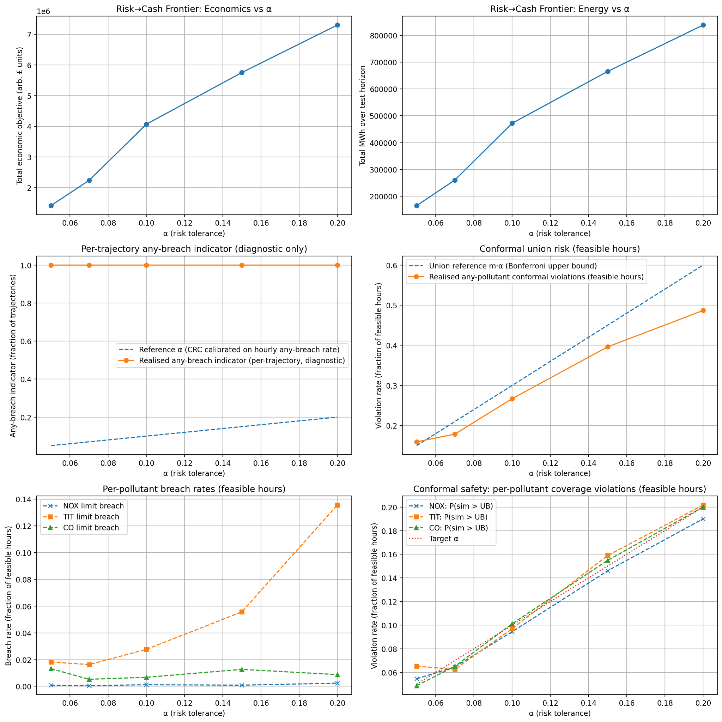
\includegraphics[width=3.36628in,height=2.23443in]{media/media/image8.png}
\caption{\protect\phantomsection\label{_Toc228132500}{}Figure 7 - CRC
Risk Calibration and Closed-Loop Breach Diagnostics}
\end{figure}

\begin{figure}
\centering
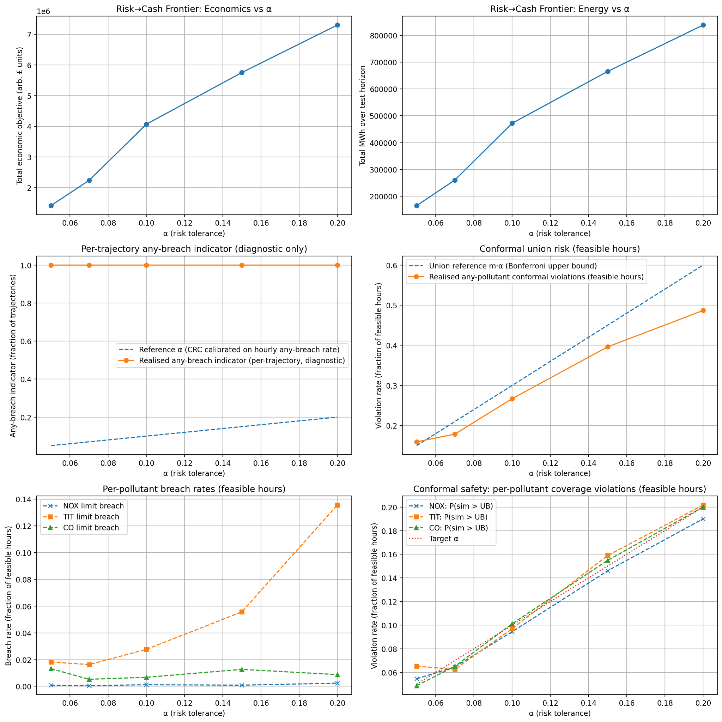
\includegraphics[width=3.28847in,height=1.08663in]{media/media/image8.png}
\caption{\protect\phantomsection\label{_Toc228132501}{}Figure 8 -
Risk--Cash Frontier Across α Risk Tolerances}
\end{figure}

With the raw upper quantile (τ = 0.95), the learned model over-covers
TIT and NOX on test (TIT empirical coverage ≈ 0.983; NOX ≈ 0.988), but
under-covers CO (empirical coverage ≈ 0.854; gap ≈ −0.096) (\emph{appx
B3)}. If interpreting this literally, the CO quantile model is too low
in the upper tail meaning it would understate risk if used as a direct
safety bound. This is consistent with CO being the most heteroscedastic
and heavy tailed target in the dataset summary.

The results show that the point-residual conformal is conservative
across the α-grid (e.g., CO point coverage stays above nominal: at
α=0.20, 0.8399 vs 0.80). However, the conformalised quantile regression,
which is meant to adapt interval width to heteroscedasticity, still
under-covers CO as α increases (CO CQR coverage falls to ≈ 0.672 at
α=0.20; gap ≈ −0.128). By contrast, NOX and TIT CQR remain close to or
above nominal at the same α values. This shows that adaptive CQR
intervals can be less conservative than residual based conformalisation.
For CO, that comes at the cost of insufficient tail buffer on the test
set.

A plausible reason as to why CO has the hardest tail is that in gas
turbines, CO rises quickly in low-temperature / low-load regimes where
oxidation is incomplete. A gas-turbine handbook notes that under
sustained low-load lean-premixed operation, CO emissions can increase
significantly due to incomplete combustion and lower combustor
temperatures (Bender, n.d.).

\subsection{Simulation}\label{simulation}

\subsubsection{CRC Risk Threshold and Closed Loop Risk
Control}\label{crc-risk-threshold-and-closed-loop-risk-control}

For each α, the code evaluates a grid of λ values over sampled
trajectories and selects the largest λ whose corrected empirical risk
satisfies the CRC criterion for the chosen loss. This distinction is
important because the CRC is designed to control the expected value of a
loss, not force the realised risk to equal a exactly at every operating
point.

\emph{Full results in this section can be found in appendix B6}

The results show that the CRC is economically consequential.

As α increases from 0.05 to 0.20, feasible operation rises from
1210/5511 hours (21.96\%) to 5474/5511 hours (99.33\%); total MWh
increases from 164,692 to 838,758; and the total economic objective
rises from about 1.42×10⁶ to 7.30×10⁶. , as seen in figure 3 below.

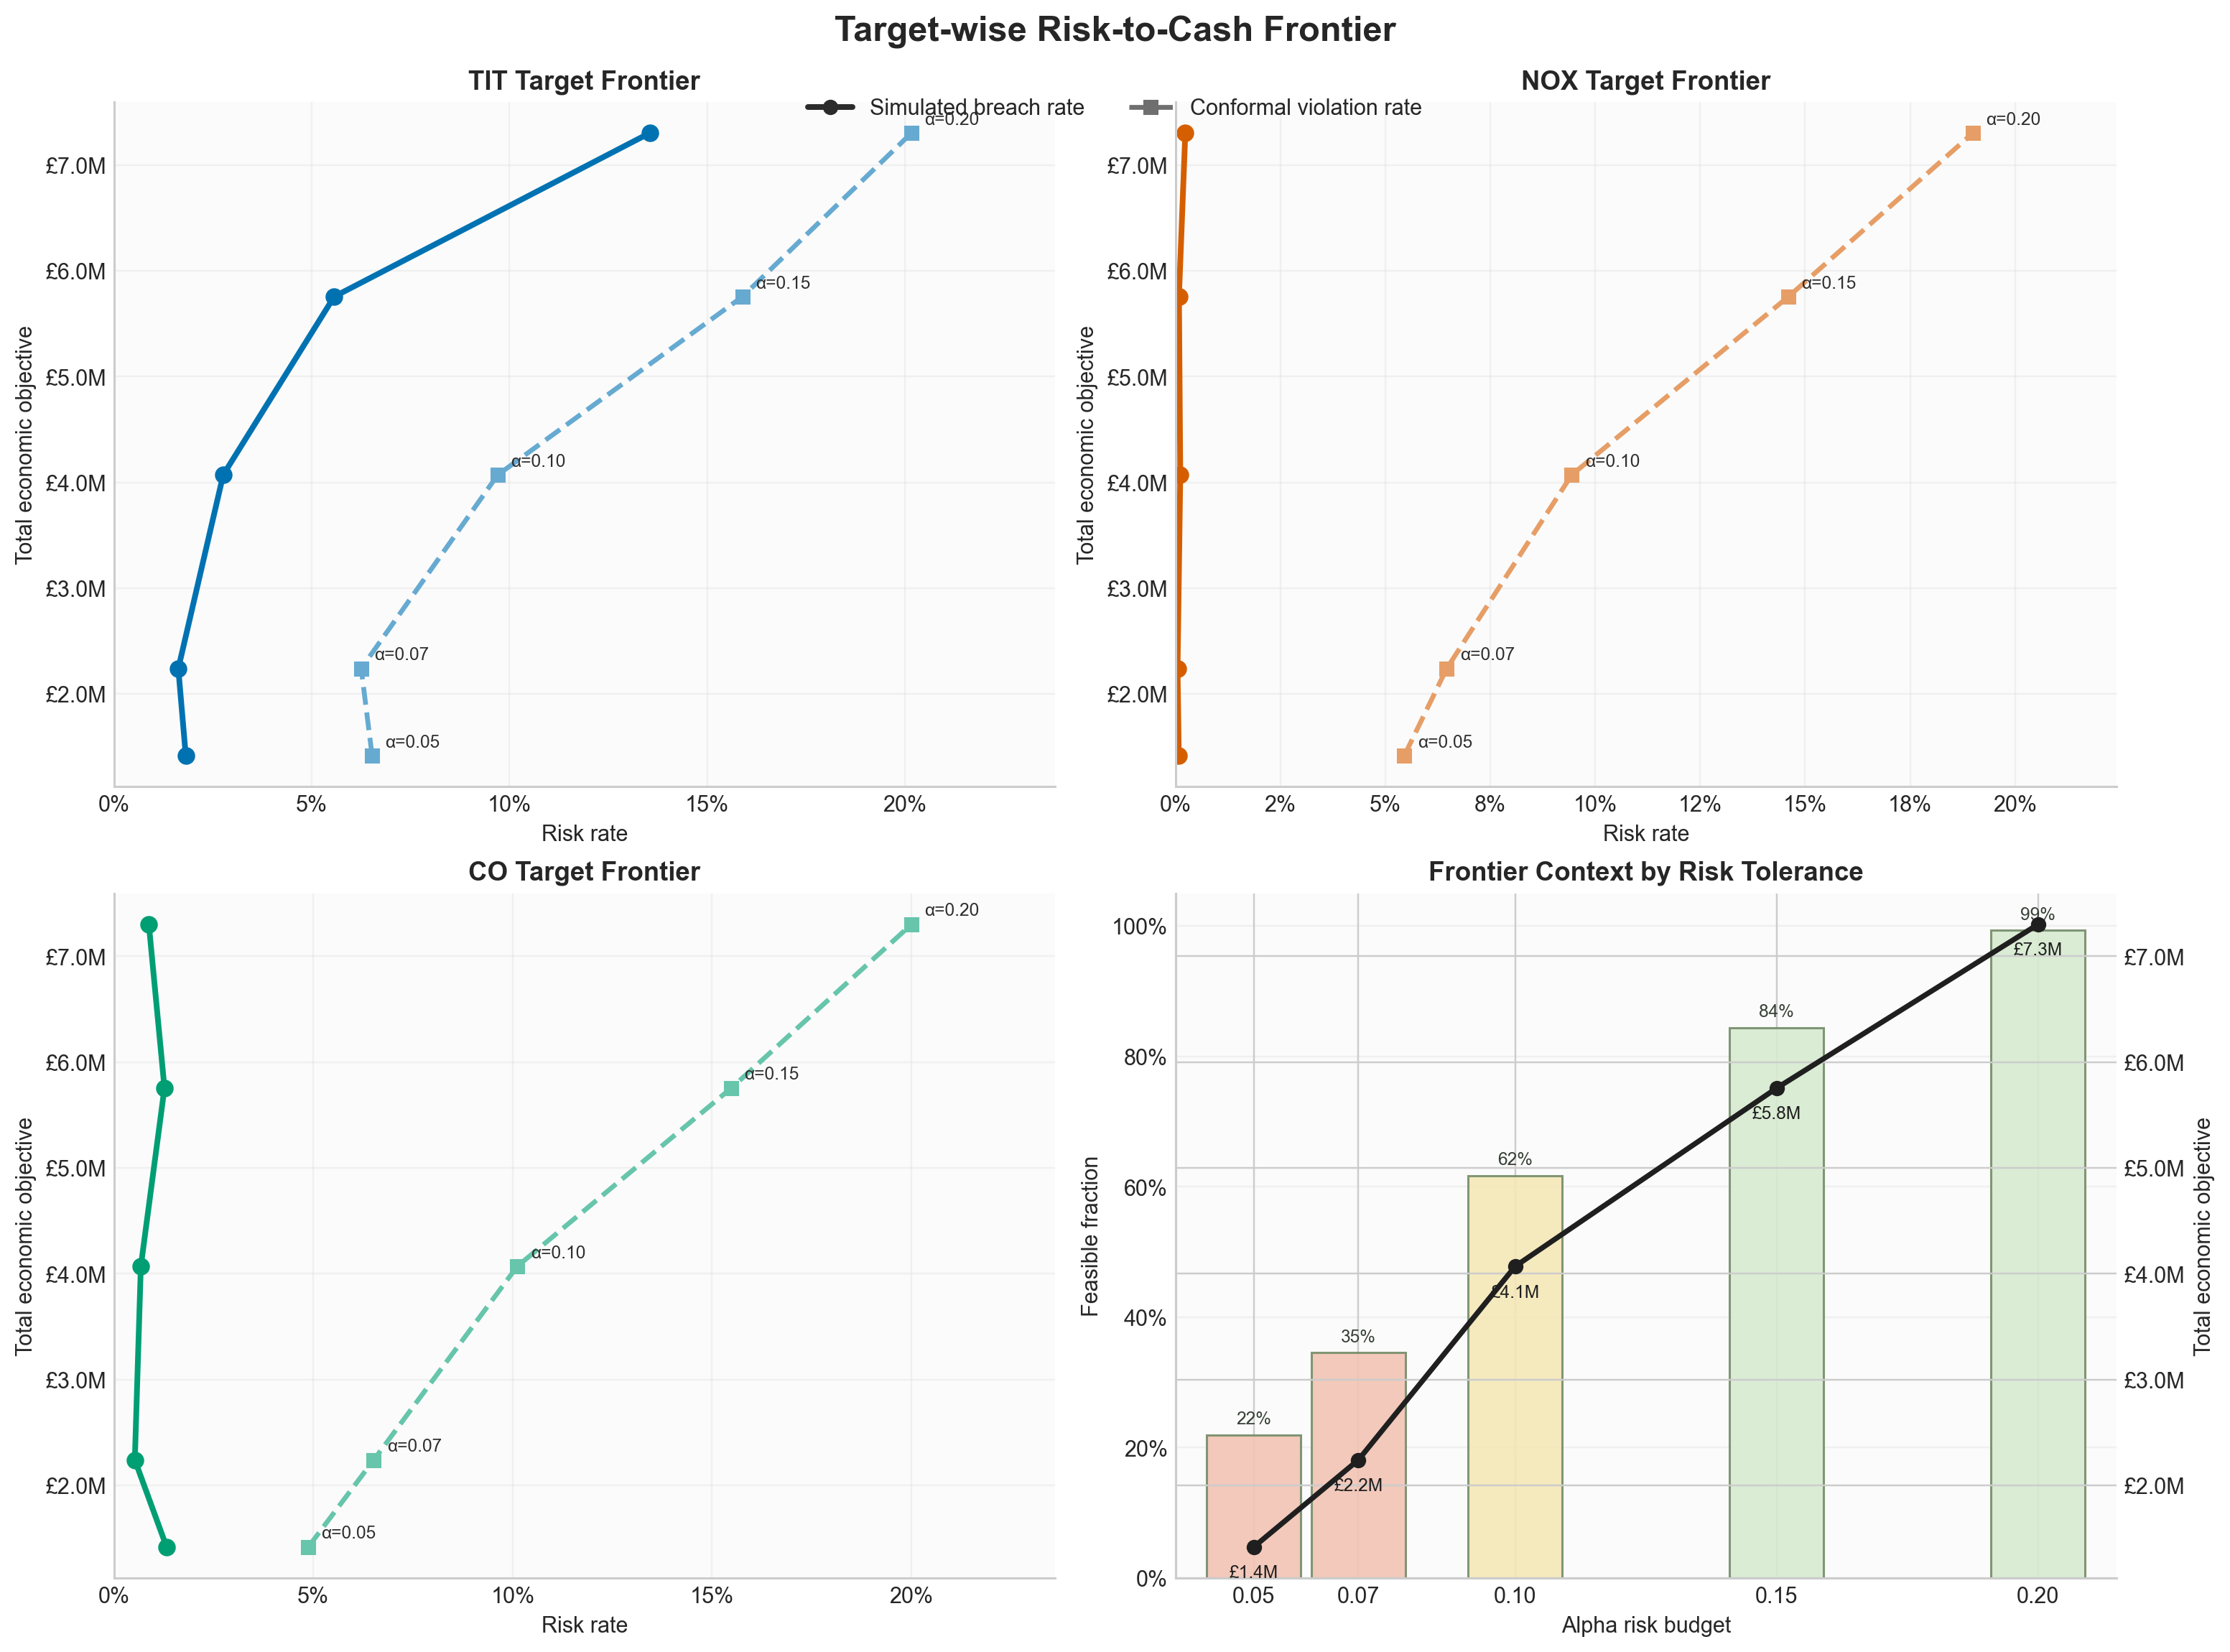
\includegraphics[width=3.16in,height=2.34056in,alt={A group of graphs showing different types of data AI-generated content may be incorrect.}]{media/media/image9.png}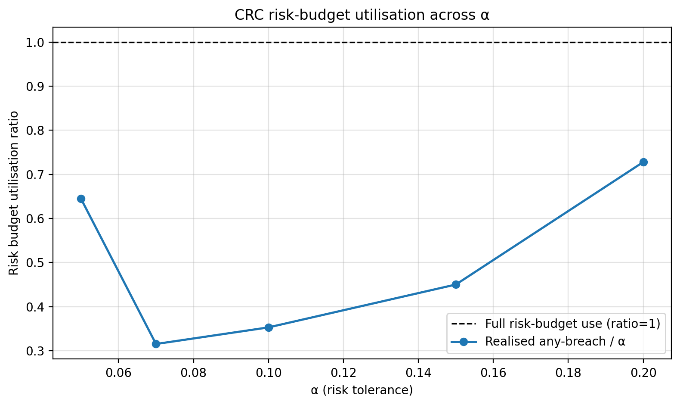
\includegraphics[width=3.23815in,height=1.92649in,alt={A graph with a line and a blue line AI-generated content may be incorrect.}]{media/media/image10.png}

\protect\phantomsection\label{_Toc228132502}{}Figure 9 - Target-Wise
Risk to Cash Frontier

\protect\phantomsection\label{_Toc228132503}{}Figure 10 - CRC
risk-budget utilisation across alpha

At the same time, any breach rates stay below the target budget tested
across the frontier: approximately 0.032, 0.022, 0.035, 0.068, 0.146 for
α = 0.05, 0.07, 0.10, 0.15, 0.20.

This corresponds to a risk budget utilisation ratio of about 0.64, 0.32,
0.35, 0.45, 0.73.

It can be said that the CRC is conservative but works for its intended
purpose. As α gets more lenient, more of the budget gets used, but is
never saturated. This is to say allowing more risk lets the controller
operate more often and earn more.

At α = 0.20, the breach rates are about 0.24\% for NOX, 0.88\% for CO,
and 13.56\% for TIT. This means that once the controller is allowed to
operate more with more risk, the residual failures are mainly thermal
instead of emission driven. This means that although the CRC is built to
screen any breach, the frontier becomes mostly shaped by the TIT risk,
increasingly as risk becomes more allowable.

It's also important to separate the idea of constraint breaches to
conformal upper bound violations. One is where the plant output exceeds
the actual defined operational limit, but upper bound violation is where
the output exceeds the predicted conformal upper bound for that hour.

At α = 0.20, the per-target conformal violation rates are close to the
target α: about 0.190, 0.202, and 0.200. But the actual breach rates are
much lower for NOX and CO. This suggests that the conformal upper bounds
are acting as a buffer zone. Crossing an upper bound happens more often
than crossing the hard safety limit itself. That is a reasonable outcome
for a safety layer built from conformal prediction, where the purpose is
calibrated protection.

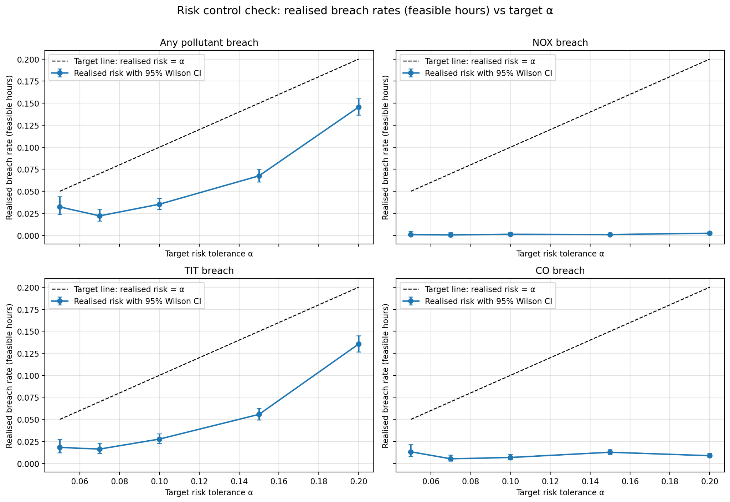
\includegraphics[width=3.14931in,height=2.16314in,alt={A graph of a graph of a person\textquotesingle s risk AI-generated content may be incorrect.}]{media/media/image11.png}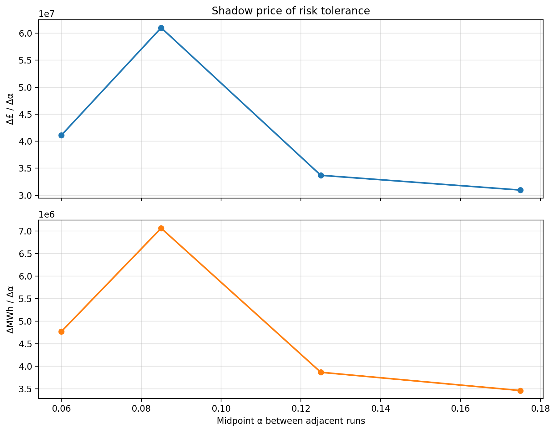
\includegraphics[width=2.88172in,height=2.23666in,alt={A graph of a graph of a line AI-generated content may be incorrect.}]{media/media/image12.png}

\protect\phantomsection\label{_Toc228132504}{}Figure 11 - Realised
Breach rates vs target alpha

\protect\phantomsection\label{_Toc228132505}{}Figure 12 - Shadow Price
of risk tolerance

It is important to interpret where exactly trade-off curve really
changes, rather than whether it just generally rises. The risk-check
plot (figure 5) uses 95\% Wilson score intervals for the hourly breach
rates, where Wilson intervals are way to put a confidence interval
around a proportion or rate - such as the breach rate or fraction of
hours with a violation, as seen in the figure above. If breaches were
observed in say 40 out of 1000 hours, the Wilson score interval gives a
plausible range for the true underlying breach probability.

In these results, the low a end is quite compressed. The hourly
any-breach rates at α=0.05, 0.07 and 0.10 are 3.22\%, 2.21\% and 3.53\%,
and their Wilson intervals overlap enough that these three settings are
not cleanly separated statistically. The higher settings, α=0.15 and
0.20, are much more clearly distinct. So, the main behavioural change
happens once the controller moves out of the row risk region, rather
than between every adjacent a.

A second point is that the operating points chosen by the controller
become more concentrated as a increases. As seen in appx B6 and
target-wise figure, the mean TEY rises from 29.88 to 152.2, however the
standard deviation falls from 56.4 to 14.4. That means that while the
controller accepts more hours, it's also generally having higher output
for these hours and more consistently allowing them. This is important
in the wider context of power generation because gas turbines are most
valuable when they can consistently hold stable high throughput
operating regime rather than jump around power outputs.

These runs of the simulator are generated from the surrogate models +
residuals, so this tighter TEY band over risk is evidence that the
surrogates are internally consistent enough to support repeated
selection of similar high-yield actions.

Figure 6 for shadow price of risk tolerance strengthens the perspective
gained in these results.

Shadow price of risk tolerance is how much extra value is gained when
the risk tolerance a is increased. It is essentially the derivative or
slope of the risk-economy curve.

The marginal gain in objective per extra unit of α is highest between
0.07 and 0.10 at about 6.10×10⁷, then drops to 3.37×10⁷ between 0.10 and
0.15 and 3.10×10⁷ between 0.15 and 0.20. The same pattern appears for
MWh. This means there is a knee (a point where the curve changes
noticeably) around α≈0.10--0.15: beyond that point, extra tolerance
still buys value, but each extra step yields less while thermal failures
rise faster. In surrogate terms, that is the key finding: the models
appear strong enough to unlock a better operating region, but under more
aggressive control the TIT tail becomes the main limit on any more
performance increases.

\subsection{Pareto Frontier}\label{pareto-frontier}

As this is a problem with multiple criteria, as discussed before, the
Pareto optimal set consists of solutions for which no objective can be
improved without worsening at least one other objective. This is
described as the pareto frontier.

Here, the optimised objective is the total economic value, and the
constrained objective is the energy weighted NOx.

The energy weighting of NOx meaning the values in the simulated NOx
series is averaged and weighted by the TEY, subject to the following
equation:

\[\text{NO}\text{x}_{\text{energy-wtd }} = \frac{\sum_{t}^{}{\text{NO}\text{x}_{\text{t}}} \cdot \text{TE}\text{Y}_{\text{t}}}{\sum_{t}^{}{\text{TE}\text{Y}_{\text{t}}}}\]

This is done because different implementations of the dispatch policy
can differ in how much energy they produce and how often they are
feasible, so it can be misleading to use absolute NOx values.

It is important to note that in these results, each e sweep is done
under the risk tolerance parameter, so the true output is not a single
frontier, but a set of frontiers indexed by the risk tolerance.

It is also noted that variable \(e\) refers to the same Pareto e, and
used in 2 different ways in the analysis.

\begin{enumerate}
\def\labelenumi{\arabic{enumi})}
\item
  ε as the swept constraint parameter
\item
  The achieved emissions value plotted on the Pareto axis.
\end{enumerate}

The code does not multiply the ε limit by a scaling factor. Instead, it
uses a separate tuning setting that changes how strongly the ε-sweep
affects the results. This setting does three things: it changes the
range of ε values tested, it changes the NOx rule used to accept or
reject candidate actions, and it increases the weight placed on NOx in
the objective during the Pareto sweep. So, this setting should be
understood as a practical tuning control for the sweep, rather than as
part of the standard ε-constraint method.

When talked about in the controller context, ε is implemented as an
additional per-hour NOX cap in the closed-loop simulation: for each ε
value you rerun EMPC+CRC ``rejecting TEY candidates whose predicted NOX
exceeds ε''.

In the results plots, when the scatter points are annotated ε=..., that
is just stating the ε value used to generate that Pareto point (i.e.,
the cap parameter for that run).

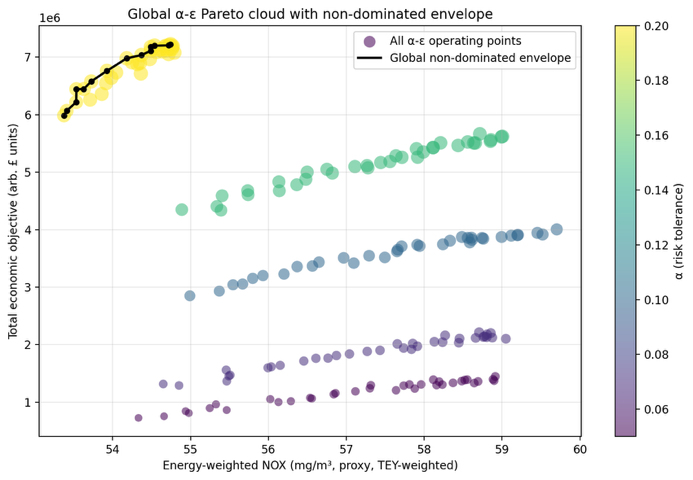
\includegraphics[width=3.13771in,height=2.17391in,alt={A graph of different colored dots AI-generated content may be incorrect.}]{media/media/image13.png}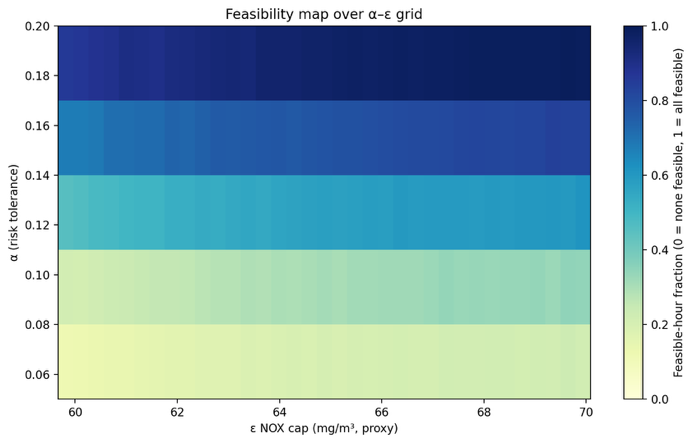
\includegraphics[width=3.25986in,height=2.08746in,alt={A chart of blue and green shades AI-generated content may be incorrect.}]{media/media/image14.png}

\protect\phantomsection\label{_Toc228132506}{}Figure 13 - Global
alpha-epsilon pareto cloud with non dominated envelope

\protect\phantomsection\label{_Toc228132507}{}Figure 14 - Feasibility
map over alpha - epsilon grid

Let us define the economic objective as \(f\).

The figure above shows each band increasing in \(f\) as NOx increases.
Within each band of risk tolerance, the curve is positively sloped:
larger NOx (looser ε since e is the right-hand side of an equality that
caps the constrained objective) corresponds to larger \(f\). This is the
expected behaviour for an ε-constraint sweep where tightening emissions
reduces the feasible set and reduces the seen values.

There is also a clear vertical separation between the risk tolerance
levels in figure 7,

At low risk tolerance (α=0.05), points occupy roughly
\(f \approx 0.7\text{–}1.4 \times 10^{6}\).

At high risk tolerance (α=0.20), points occupy roughly
\(f \approx 6.0\text{–}7.3 \times 10^{6}\)

This shows that risk tolerance is the primary driver of the achieved
total value, rather than e alone, over the tested values.

It is also important to note that in figure 7, the α = 0.20 band has a
low NOx (≈53--55 mg/m³) while also having higher value than lower-α
bands. That means that a is changing which operating regimes are
reachable under the risk constraints, making potentially more efficient
decisions.

Figure 8 shows the fraction of feasible hours over the pareto sweep. The
main effect is vertical gradient change where at α≈0.06--0.08,
feasibility is low, and at α=0.20, feasibility is near full. Contrasting
this, increasing ε at fixed α gives a smaller feasibility gain, for
example along a =0.1, feasibility rises only slightly though the e
values. This is consistent with the idea that α primarily determines if
the controller finds feasible operation for a large portion of the
horizon, whereas ε primarily determines where on the curve the feasible
operation lands once feasibility is already considered.

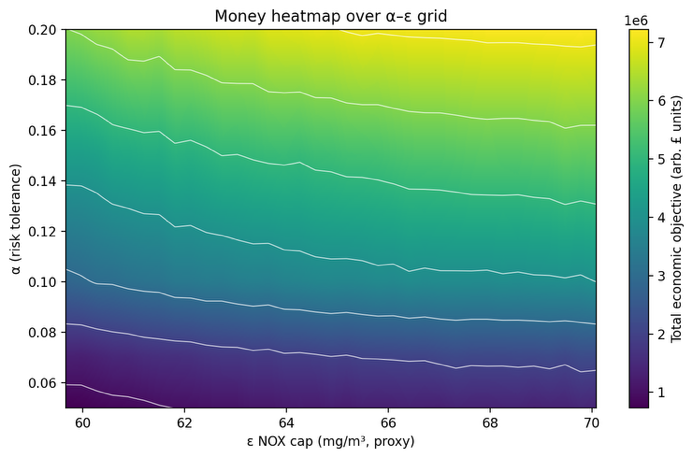
\includegraphics[width=3.14931in,height=2.07986in,alt={A graph showing the heatmap over a grid AI-generated content may be incorrect.}]{media/media/image15.png}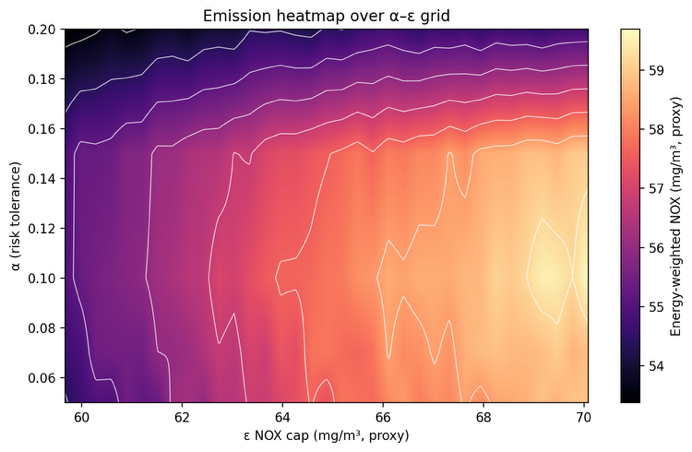
\includegraphics[width=3.14931in,height=2.05278in,alt={A graph of a heatmap AI-generated content may be incorrect.}]{media/media/image16.png}

\protect\phantomsection\label{_Toc228132508}{}Figure 15 - Money heatmap
over alpha-epsilon grid

\protect\phantomsection\label{_Toc228132509}{}Figure 16 - Emission
heatmap over alpha-epsilon grid

Figure 9 is globally smooth and monotone, \(f\) increases strongly with
a and more mildly with e. The iso contours slope downwards, which infers
that there's a partial substitutability. A higher e can compensate (to
some extent) for a stricter risk tolerance, but not fully in the context
of this implementation. The emission heatmap shows that achieved
energy-weighted NOx in roughly the 53--60 mg/m³ range. Achieved NOX
rises with ε (as expected), but it also varies with α, implying that the
risk controller changes operating regimes in a way that affects the
realized emissions distribution.

\begin{figure}
\centering
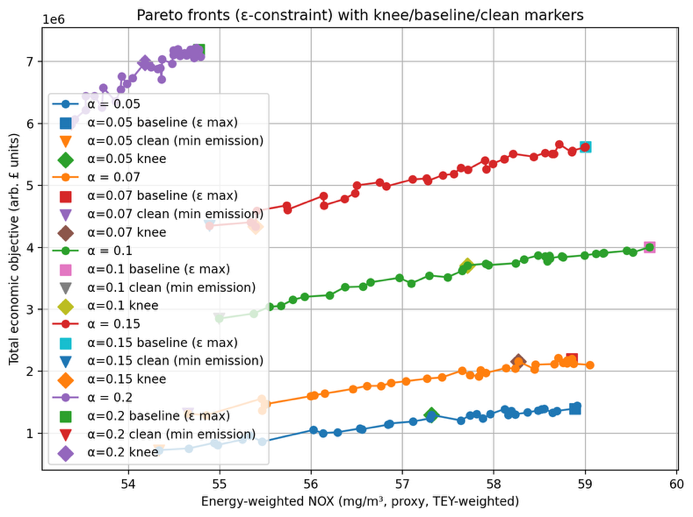
\includegraphics[width=3.1489in,height=2.35039in,alt={A graph of different colored lines AI-generated content may be incorrect.}]{media/media/image17.png}
\caption{\protect\phantomsection\label{_Toc228132510}{}Figure 17 -
Pareto Fronts with knee/baseline/clean markers}
\end{figure}

Knee points can make areas with high marginal utility obvious. These are
areas where small gains in one objective would require
disproportionately large sacrifices in the other (as previously
mentioned).

In figure 11, for α=0.10 (green curve), the markers imply approximately:

\begin{itemize}
\item
  Baseline: NOX ≈ 59.7 mg/m³, \(f \approx 4.0 \times 10^{6}\).
\item
  Clean: NOX ≈ 55.0 mg/m³, \(f \approx 2.85 \times 10^{6}\).
\item
  Knee: NOX ≈ 57.7 mg/m³, \(f \approx 3.7 \times 10^{6}\).
\end{itemize}

This implies a trade-off:

\begin{itemize}
\item
  Baseline → Clean: abatement \(\Delta E \approx 4.7\)mg/m³ for value
  loss \(\Delta f \approx 1.15 \times 10^{6}\).
\item
  Baseline → Knee: abatement \(\Delta E \approx 2.0\)mg/m³ for value
  loss \(\Delta f \approx 0.3 \times 10^{6}\).
\end{itemize}

This is to say that the knee point captures \textasciitilde43\% of the
abatement for \textasciitilde26\% of the value loss, which is a
mechanism that is useful when optimising the controller to search for
points of maximum interest and value to an operator.

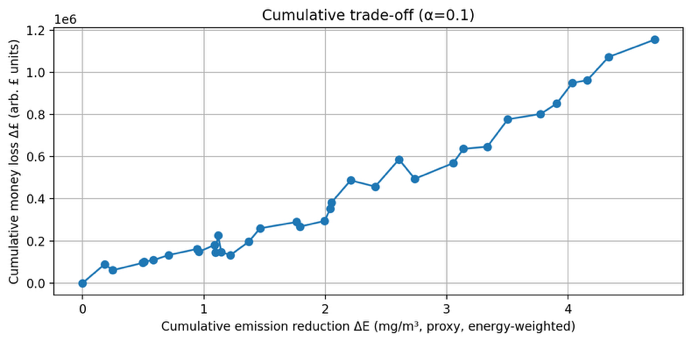
\includegraphics[width=3.14931in,height=1.55278in,alt={A graph with blue lines and numbers AI-generated content may be incorrect.}]{media/media/image18.png}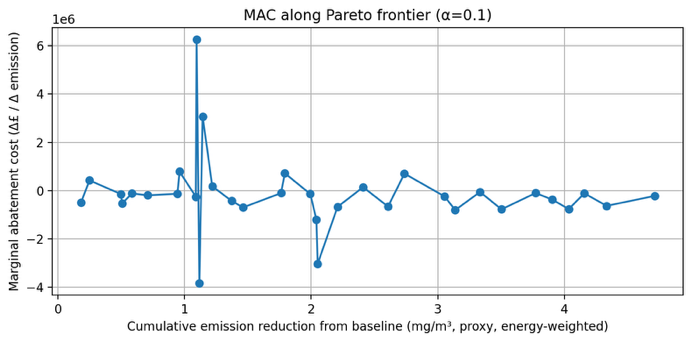
\includegraphics[width=3.14931in,height=1.55278in,alt={A graph with blue lines and dots AI-generated content may be incorrect.}]{media/media/image19.png}

\protect\phantomsection\label{_Toc228132511}{}Figure 18 - Cumulative
trade-off at alpha = 0.1

\protect\phantomsection\label{_Toc228132512}{}Figure 19 - MAC along
Pareto frontier at alpha = 0.1

The figure 12, cumulative trade at a= 0.10 continues to reinforce the
same evidence, that cumulative money loss \(\Delta f\)increases to
\textasciitilde{}\(1.15 \times 10^{6}\) as cumulative NOX reduction
\(\Delta E\) reaches \textasciitilde4.7 mg/m³, with smaller local areas
non-monatomicities. This could be due to

(i) simulation noise and finite-sample estimation: each frontier point
is based on a single closed-loop simulated rollout, so small random
differences in realised outcomes can make neighbouring ε points swap
order slightly. This is a standard issue in simulation-based
optimisation unless you average over multiple replications (Kim et al.,
2011) .

(ii) finite-difference amplification in MAC: your MAC curve is computed
from adjacent-point ratios \(\Delta f/\Delta E\), so when two
neighbouring points have very small \(\Delta E\), even tiny noise in
\(f\)produces large spikes or sign flips. Finite-difference derivatives
are well known to be unstable under noisy function evaluations. This is
the likely cause the outlier in the figure below (Kim et al., 2011).

Figure 13 estimates the marginal abatement cost \((\Delta f/\Delta E)\)
. In literature, the MAC (marginal abatement cost) is a defined as the
cost associated with the last unit of abatement for varying amounts of
abatement. The plot shows sharp spikes in positive and negative
directions around ΔE≈1.1 mg/m³, which implies that adjacent sampled
points sometimes change 𝑓 and NOx in inconsistent directions. This alone
doesn't necessary render the analyse invalid, but it does show that the
local slope estimates are sensitive to discretization and simulation
noise. Literature explores this and cautions against over-interpreting
curve details (Kesicki and Ekins, 2012).

\section{The Wider Context}\label{the-wider-context}

\section{}\label{section-13}

\subsection{Interpretation of results}\label{interpretation-of-results}

The main value of the method is that it protects decision-making under
uncertainty. In a constrained controller, performance depends on how
many actions are still allowed after the safety and emissions checks are
applied. When the uncertainty margin changes, that feasible set can
change quickly. A small statistical change can therefore create a large
operational change. This is consistent with how constrained predictive
control works, where different active constraints create different
decision regions, and with the wider idea of a safe operating envelope.

This gives a more useful reading of the risk--value trade-off in this
dissertation. At first, relaxing the risk setting gives the controller
back real freedom. More actions remain feasible, so the plant can use a
wider and more valuable part of its operating range. After that, the
gains become smaller. The controller is mostly choosing between similar
actions, while the same hard limit still dominates. In that sense, CRC
is a practical way to manage the safe operating envelope of the plant.

This interpretation is useful because it changes how the method should
be tuned. The main concern becomes also how much operating freedom
remains after the uncertainty margin is applied. In practice, that means
the method should be judged using measures such as the number of
feasible candidate actions, the spread of accepted actions, and which
constraint is active most often. Those measures would show whether the
controller is still making meaningful choices, or whether it has become
safe mainly by removing too much of the operating space.

\subsection{}\label{section-14}

\subsection{Operational Translation of
Variables}\label{operational-translation-of-variables}

For translating the methodology to other contexts, it must be understood
that the risk is a frequency of adverse events under the decision maker.
This is what would be considered the main transferable conceptual
element.

In an industrial setting, the operator often acts a risk manager of an
operating envelope. They decide how close the plant runs to defined
limits, how much to tolerate overruns, and what operation matters for
compliance etc (Senthilvelan et al., 2025a).

In the implementation `cash' or `economy' is a placeholder proxy for
economic utility. It is the quantity traded off against constraint risk.
To generalise to other deployments, operators can reinterpret the
objective as any operation value function that the organisation
recognises and care abouts. This could be profit, fuel cost, carbon
cost, availability value etc. Real world optimization is often similarly
framed as maximising operation profit due to changing conditions and
constraints (Eker and Taware, 2003).

A transfer is the comparative idea that increasing tolerance for
constraint risk expands the reachable operating region, but with
diminishing marginal returns beyond a knee. The results of the project
already quantify the knee for the setup, but an operator in a different
plant could reuses the interpretation where spending more of a
predefined budget may yield less value because another constraint or
failure mode becomes binding.

In the project, feasibility is the existence of at least on candidate
action that passes the constraint checks at each time step. In terms of
a real-world operator, this can be interpreted as the operation
headroom. A high feasible fraction means the current policies still
leave the plan room to make more decisive decisions, and a low feasible
fraction means the constraint set is incompatible with the target region
given the disturbances and modelling error.

Conceptually, this alignment matches how safe operating limits are
treated in safety processes, where limits define an allowable operating
region, and a policy is derived that leaves a margin, so disturbances
don't cause failures (Senthilvelan et al., 2025b).

The results already show a generalisable pattern that feasibility is
governed by risk tolerance, and change a fixed parameter e at fixed a
has smaller feasibility gains. This could be interpreted by an operator
as the risk tolerance controls whether the controller can reliable find
admissible operating regions across the horizon, while e selects which
admissible regime is chosen once admissibility is common and acceptable.

The results show how an operator can reason with the risk tolerance. The
knee around a = 0.1 -- 0.15 indicates a point where relaxing risk
tolerance yields diminishing marginal value and rising thermal-limit
issues. In another plant, the knee might occur elsewhere and might be
driven by different constraints. The logic however remains the same.

In terms of the interpretability of the CRC threshold (considered λ), it
is a threshold based on a risk score so that the empirical risk of a
chosen loss stays below a in expectation.

In operator terms, λ could generalise into a boundary used in screening,
where actions with sufficiently high predicted risk are excluded from
consideration. Due to the fact the CRC is explicitly designed to be
meaningful under certain types of distribution shift, λ can also be read
as a closed loop robustness variable as it is calibrated on trajectories
that reflect the policies behaviour. This is recognised issue in
performative prediction where changing targets induce a shift in
operation (J. Perdomo et al., 2020).

The ``learned safety margin'' of the conformal prediction is especially
relevant for emissions because real emissions monitoring and compliance
checking explicitly deal with measurement uncertainty and instrument
drift/quality assurance. Guidance documents describe how uncertainty is
assessed and how compliance against emission limit values (ELVs) should
account for it. The conformal margin can be interpreted as a data-driven
analogue of the uncertainty buffer that compliance frameworks already
recognise (Environment Agency and United Kingdom Government, 2025).

\subsection{\texorpdfstring{Failure Modes and Shortcomings
}{Failure Modes and Shortcomings }}\label{failure-modes-and-shortcomings}

It could be said that some patterns in the results set are driven by the
decision-making process as much as the actual turbine behaviour. The
controller never optimises over a smooth region, it's always a discrete
grid of TEY options, that is reduced by set of filters. This means small
changes in modelling or calibration can likely produce large changes in
the number of feasible hours and in turn the performance of the turbine.

A major shortcoming of this implementation of the methodology is how
conservative the model can be from the stacking of the safety layers.
Conformal bounds already widen predictions to prevent against errors in
the tails, and then CRC could reject them again based on its own learned
criteria. When these layers overlap, the feasible set can shrink for
reasons that aren't based on true operational choices, but just through
the construction of the method.

If a single blocker dominates the regime, then the frontier can be more
representative of the methodological choices rather than the
relationship you're really looking for.

The CRC introduces another failure mode. It relies on the ranking
quality of the risk score more than on real probabilities. If
exceedances of these values are, rare, the breach classifiers can rank
near boundary cases poorly. This matters because the optimiser tends to
operate near constraints. If this is the case, then a may not translate
cleanly into different realised risk levels even if the calibration is
correct.

Another shortcoming of the method comes from the simulation. The closed
loop process adds residuals per target the resampled independently. This
can make cross target dependence lose value and reduce the effect of
temporal persistence, which can negatively affect results.

\section{Conclusion}\label{conclusion}

\section{}\label{section-15}

The project shows that managing uncertainty alters the feasible action
set of gas turbine operation, thus changing the operation policy and
value. In this context, conformal bounds and the CRC gate played an
important role, as they determined the potential for economically viable
dispatch.

As risk tolerance increased, both feasibility and economic value
increased, but these gains were not linear.

A noticeable point emerged around α ≈ 0.10--0.15. Beyond this, taking on
more risk yielded diminishing returns while the likelihood of thermal
failures grew rapidly. This indicates that TIT, rather than emissions
alone, became the primary limiting factor.

Furthermore, the results suggest that average prediction accuracy
isn\textquotesingle t enough to evaluate models ready for control. While
TIT was the easiest to learn, NOx proved structurally hard to predict,
and CO was the most difficult to reliably bound at high levels. However,
closed-loop performance hinged more on behaviour near constraint
boundaries than on overall error metrics.

These findings should be approached critically. The described issues
such as using proxy economics, proxy limits, and a limited scope dataset
means that the results are not necessarily generalisable.

This work could be improved if it could be tested under broader evidence
base; such as a larger dataset or data from different turbines in
different environments rather than relying on a single dataset. Future
work should model the dependence between TIT, NOx and CO more
explicitly, because the current target-wise surrogates and breach models
only capture this indirectly, and CO was the hardest variable to bound
reliably in the upper tail. The work could be extended to work with
different surrogate models and NN's and could also be introduced into a
live setting where new data is sequentially added during operation to
explore findings in that space.

\section{Bibliography}\label{bibliography}

\section{}\label{section-16}

Ames Research Staff, B., Field, M., n.d. EQUATIONS, TABLES, AND CHARTS
FOR COMPRESSIBLE FLOW.

\begin{quote}
Angelopoulos, A.N., Bates, S., 2022. A Gentle Introduction to Conformal
Prediction and Distribution-Free Uncertainty Quantification.

Angelopoulos, A.N., Bates, S., Fisch, A., Lei, L., Schuster, T., 2025.
Conformal Risk Control.

Arrigo, A., Ordoudis, C., Kazempour, J., De Grève, Z., Toubeau, J.F.,
Vallée, F., 2022. Wasserstein distributionally robust chance-constrained
optimization for energy and reserve dispatch: An exact and
physically-bounded formulation. Eur. J. Oper. Res. 296, 304--322.
https://doi.org/10.1016/j.ejor.2021.04.015

Asif, M., Amin, A., Jamil, U., Mahmood, A., Ahmed, U., Razzaq, S.,
Mahdi, F.P., 2024. Combined emission economic dispatch using
quantum-inspired particle swarm optimization and its variants. Energy
Exploration and Exploitation 42, 1602--1644.
https://doi.org/10.1177/01445987241235419

Bender, Wi.R., n.d. 3.2.1.2 Lean Pre-Mixed Combustion 3.2.1.2-1
Introduction 3.2.1.2-2 Emissions Overview.

Clarke, D.R., Levi, C.G., 2003. Materials Design for the Next Generation
Thermal Barrier Coatings. Annu. Rev. Mater. Res. 33, 383--417.
https://doi.org/10.1146/annurev.matsci.33.011403.113718
\end{quote}

Collins, G.S., Moons, K.G.M., Dhiman, P., Riley, R.D., Beam, A.L., Van
Calster, B., Ghassemi, M., Liu, X., Reitsma, J.B., Van Smeden, M.,
Boulesteix, A.L., Camaradou, J.C., Celi, L.A., Denaxas, S., Denniston,
A.K., Glocker, B., Golub, R.M., Harvey, H., Heinze, G., Hoffman, M.M.,
Kengne, A.P., Lam, E., Lee, N., Loder, E.W., Maier-Hein, L., Mateen,
B.A., McCradden, M.D., Oakden-Rayner, L., Ordish, J., Parnell, R., Rose,
S., Singh, K., Wynants, L., Logullo, P., 2024. TRIPOD+AI statement:
Updated guidance for reporting clinical prediction models that use
regression or machine learning methods. BMJ.
https://doi.org/10.1136/bmj-2023-078378

Dixit, A., Lindemann, L., Wei, S.X., Cleaveland, M., Pappas, G.J.,
Burdick, J.W., 2023. Adaptive Conformal Prediction for Motion Planning
among Dynamic Agents, in: Matni, N., Morari, M., Pappas, G.J. (Eds.),
Proceedings of The 5th Annual Learning for Dynamics and Control
Conference, Proceedings of Machine Learning Research. PMLR, pp.
300--314.

\begin{quote}
dos Santos Coelho, L., Hultmann Ayala, H.V., Cocco Mariani, V., 2024a.
CO and NOx emissions prediction in gas turbine using a novel modeling
pipeline based on the combination of deep forest regressor and feature
engineering. Fuel 355. https://doi.org/10.1016/j.fuel.2023.129366

dos Santos Coelho, L., Hultmann Ayala, H.V., Cocco Mariani, V., 2024b.
CO and NOx emissions prediction in gas turbine using a novel modeling
pipeline based on the combination of deep forest regressor and feature
engineering. Fuel 355, 129366.
https://doi.org/10.1016/j.fuel.2023.129366
\end{quote}

Efron, B., 1979. Bootstrap Methods: Another Look at the Jackknife.

Eker, S.A., Taware, A., 2003. REAL-TIME OPTIMAL OPERATION DECISIONS FOR
GAS TURBINES.

Enviroment Agency, United Kingdom Government, 2025. Monitoring stack
emissions: quality assurance of continuous monitoring {[}WWW
Document{]}. GOV.UK.

Fontana, M., Zeni, G., Vantini, S., 2023. Conformal prediction: A
unified review of theory and new challenges. Bernoulli 29, 1--23.
https://doi.org/10.3150/21-BEJ1447

\begin{quote}
Förtsch, D., 2025. On the dependencies of the average specific heat
capacity of flue gas. Fuel Communications 23, 100136.
https://doi.org/10.1016/j.jfueco.2025.100136

Foygel Barber, R., Candès, E.J., Ramdas, A., Tibshirani, R.J., 2021. The
limits of distribution-free conditional predictive inference.
Information and Inference 10, 455--482.
https://doi.org/10.1093/imaiai/iaaa017
\end{quote}

Freedman, D.A., 1981. Bootstrapping Regression Models, Source: The
Annals of Statistics.

Gibbs, I., Candès, E., 2021. Adaptive Conformal Inference Under
Distribution Shift.

Grinsztajn, L., Oyallon, E., Varoquaux, G., 2022. Why do tree-based
models still outperform deep learning on tabular data?

Hewamalage, H., Ackermann, K., Bergmeir, C., 2023. Forecast evaluation
for data scientists: common pitfalls and best practices. Data Min.
Knowl. Discov. 37, 788--832. https://doi.org/10.1007/s10618-022-00894-5

\begin{quote}
Hu, Y., Li, Y., Xu, M., Zhou, L., Cui, M., 2017. A chance-constrained
economic dispatch model in wind-thermal-energy storage system. Energies
(Basel). 10. https://doi.org/10.3390/en10030326

Jhinaoui, A., Malkogianni, A., City, M., Dhabi, A., Hasani Azamar, U.,
Tsoutsanis, E., n.d. ATTENTIONAL NEURAL NETWORK FOR THE PREDICTION OF
GAS TURBINE CO AND NOx EMISSION.
\end{quote}

Jhinaoui, A., Malkogianni, A., City, M., Dhabi, A., Hasani Azamar, U.,
Tsoutsanis, E., n.d. ATTENTIONAL NEURAL NETWORK FOR THE PREDICTION OF
GAS TURBINE CO AND NOx EMISSION.

Ke, G., Meng, Q., Finley, T., Wang, T., Chen, W., Ma, W., Ye, Q., Liu,
T.-Y., n.d. LightGBM: A Highly Efficient Gradient Boosting Decision
Tree.

Kesicki, F., Ekins, P., 2012. Marginal abatement cost curves: a call for
caution. Climate Policy 12, 219--236.
https://doi.org/10.1080/14693062.2011.582347

Kesicki, F., Strachan, N., 2011. Marginal abatement cost (MAC) curves:
confronting theory and practice. Environ. Sci. Policy 14, 1195--1204.
https://doi.org/10.1016/j.envsci.2011.08.004

\begin{quote}
Kim, S., Pasupathy, R., Henderson, S.G., 2011. A Guide to Sample-Average
Approximation.

Lei, J., G'sell, M., Rinaldo, A., Tibshirani, R.J., Wasserman, L., n.d.
Distribution-Free Predictive Inference for Regression.
\end{quote}

Lindemann, L., Cleaveland, M., Shim, G., Pappas, G.J., 2023a. Safe
Planning in Dynamic Environments using Conformal Prediction.

Lindemann, L., Cleaveland, M., Shim, G., Pappas, G.J., 2023b. Safe
Planning in Dynamic Environments Using Conformal Prediction. IEEE Robot.
Autom. Lett. 8, 5116--5123. https://doi.org/10.1109/LRA.2023.3292071

\begin{quote}
Lipperheide, M., Gassner, M., Weidner, F., Bernero, S., Wirsum, M.,
2018. Long-term carbon monoxide emission behavior of heavy-duty gas
turbines: An approach for model-based monitoring and diagnostics.
International Journal of Spray and Combustion Dynamics 11.
https://doi.org/10.1177/1756827718791921

Marouani, I., Guesmi, T., Abdallah, H.H., Alshammari, B.M., Alqunun, K.,
Alshammari, A.S., Rahmani, S., 2022. Combined Economic Emission Dispatch
with and without Consideration of PV and Wind Energy by Using Various
Optimization Techniques: A Review. Energies (Basel).
https://doi.org/10.3390/en15124472
\end{quote}

Mavrotas, G., 2009. Effective implementation of the ε-constraint method
in Multi-Objective Mathematical Programming problems. Appl. Math.
Comput. 213, 455--465. https://doi.org/10.1016/j.amc.2009.03.037

Mcbride, B.J., Zehe, M.J., Gordon, S., 2002. NASA Glenn Coefficients for
Calculating Thermodynamic Properties of Individual Species.

\begin{quote}
Pachauri, N., 2024. An emission predictive system for CO and NOx from
gas turbine based on ensemble machine learning approach. Fuel 366,
131421. https://doi.org/10.1016/j.fuel.2024.131421

Perdomo, J., Zrnic, T., Mendler-Dünner, C., Hardt, M., 2020.
Performative Prediction, in: III, H.D., Singh, A. (Eds.), Proceedings of
the 37th International Conference on Machine Learning, Proceedings of
Machine Learning Research. PMLR, pp. 7599--7609.
\end{quote}

Perdomo, J.C., Zrnic, T., Mendler-D ¨, C., Hardt, M., 2020. Performative
Prediction.

Potts, R., Hackney, R., Leontidis, G., 2023. Tabular Machine Learning
Methods for Predicting Gas Turbine Emissions. Mach. Learn. Knowl. Extr.
5, 1055--1075. https://doi.org/10.3390/make5030055

Richards, G., Weiland, N., Strakey, P., n.d. Combustion Strategies for
Syngas and High-Hydrogen Fuel.

Romano, Y., Patterson, E., Candès, E.J., n.d. Conformalized Quantile
Regression.

\begin{quote}
Saravanamuttoo, H.I.H.., 2017. Gas turbine theory. Pearson.

Senthilvelan, K., Shaik, S.M., Wong, W.C., Sugiman, D., 2025a. From
theory to practice: Implementing safe operating limits in major hazard
facilities. Process Safety Progress 44, 553--563.
https://doi.org/10.1002/prs.70031
\end{quote}

Senthilvelan, K., Shaik, S.M., Wong, W.C., Sugiman, D., 2025b. From
theory to practice: Implementing safe operating limits in major hazard
facilities. Process Safety Progress 44, 553--563.
https://doi.org/10.1002/prs.70031

Shafer, G., Vovk, V., 2008. A Tutorial on Conformal Prediction, Journal
of Machine Learning Research.

Tibshirani, R.J., Barber, R.F., Candès, E.J., Ramdas, A., 2019.
Conformal prediction under covariate shift, in: Proceedings of the 33rd
International Conference on Neural Information Processing Systems.
Curran Associates Inc., Red Hook, NY, USA.

UCI Machine Learning Repository, 2019. Gas Turbine CO and NOx Emission
Data Set.

\begin{quote}
United States Department of Energy, 2022. A LITERATURE REVIEW OF
HYDROGEN AND NATURAL GAS TURBINES: CURRENT STATE OF THE ART WITH REGARD
TO PERFORMANCE AND NO X CONTROL A LITERATURE REVIEW OF HYDROGEN AND
NATURAL GAS TURBINES: CURRENT STATE OF THE ART WITH REGARD TO
PERFORMANCE AND NOX CONTROL 1.

United States Environmental Protection Agency, 2025a. Nitrogen Dioxide
(NO2) Pollution {[}WWW Document{]}.
https://www.epa.gov/no2-pollution/basic-information-about-no2?utm\_source=chatgpt.com.
\end{quote}

United States Environmental Protection Agency, 2025b. Carbon Monoxide
(CO) Pollution in Outdoor Air {[}WWW Document{]}.
https://www.epa.gov/co-pollution/basic-information-about-carbon-monoxide-co-outdoor-air-pollution?utm\_source=chatgpt.com.

Unnikrishnan, U., Yang, V., 2022. A review of cooling technologies for
high temperature rotating components in gas turbine. Propulsion and
Power Research. https://doi.org/10.1016/j.jppr.2022.07.001

Winkler Dieter~ and Geng, W. and E.G. and S.P. and K.K. and G.T., 2017.
Staged combustion concept for gas turbines. Journal of the Global Power
and Propulsion Society 1, 184--194. https://doi.org/10.22261/CVLCX0

\begin{quote}
Xu, C., Xie, Y., 2021. Conformal Prediction Interval for Dynamic
Time-Series.

Yang, Y., Nikolaidis, T., Jafari, S., Pilidis, P., 2024. Gas turbine
engine transient performance and heat transfer effect modelling: A
comprehensive review, research challenges, and exploring the future.
Appl. Therm. Eng. 236, 121523.
https://doi.org/10.1016/j.applthermaleng.2023.121523
\end{quote}

~

\section{}\label{section-17}

\section{Appendices}\label{appendices}

\section{}\label{section-18}

\subsection{A: Pseudocode summary of main algorithms used in
codebase}\label{a-pseudocode-summary-of-main-algorithms-used-in-codebase}

\section{}\label{section-19}

\textbf{A1 -- Surrogate model training}

\begin{quote}
ALGORITHM train\_surrogates():

~~// ── Load pre-built feature artifact (written by surrogate\_model.py)
──

~~prepared ~ ←
load\_prepared\_feature\_artifact(PREPARED\_FEATURES\_PATH)

~~df ~ ~ ~ ~ ← prepared{[}\textquotesingle df\textquotesingle{]}

~~X~ ~ ~ ~ ~ ← prepared{[}\textquotesingle X\textquotesingle{]}~ ~ ~ ~ ~
~ ~ ~ ~ ~ ~ // full feature matrix

~~m\_train~ ~ ←
prepared{[}\textquotesingle mask\_train\textquotesingle{]}~ ~ ~ ~ ~ ~ ~
// bool mask, 70\% of rows

~~m\_calib~ ~ ←
prepared{[}\textquotesingle mask\_calib\textquotesingle{]}~ ~ ~ ~ ~ ~ ~
// bool mask, 15\% of rows

~~target\_feature\_map ←
prepared{[}\textquotesingle target\_feature\_map\textquotesingle{]}

~~~~// \{TIT: {[}...{]}, NOX: {[}...{]}, CO: {[}...{]}\}

~~~~// TIT: base\_exog + time\_feats + lag1 of \{TEY,TIT,GTEP,TAT,CDP\}

~~~~// NOX: TIT features + NOX history lags \{1,2,3\}

~~~~// CO : NOX features + CO history lags \{1,2,3,6,12,24\}

~~// ── Leakage guard
─────────────────────────────────────────────────────

~~assert \{TIT, TAT, GTEP, CDP\} ∩ features = ∅~ ~ // current-step
outputs excluded

~~assert TIT\_lag1 ∈
target\_feature\_map{[}\textquotesingle TIT\textquotesingle{]}

~~assert NOX\_lag1 ∈
target\_feature\_map{[}\textquotesingle NOX\textquotesingle{]}

~~assert CO\_lag1~ ∈
target\_feature\_map{[}\textquotesingle CO\textquotesingle{]}

~~X\_train ← X{[}m\_train{]};~ X\_calib ← X{[}m\_calib{]}

~~for target in \{TIT, NOX, CO\}:

~~~~feats~ ~ ← target\_feature\_map{[}target{]}

~~~~X\_tr\_all ← X\_train{[}feats{]} ~ ~ ~ ~ ~ ~ ~ ~ ~ ~ //
target-specific columns only

~~~~y\_tr\_all ← df{[}target{]}{[}m\_train{]}

~~~~// Inner temporal validation split (last 10\% of train, min 200
rows)

~~~~n\_val ~ ~ ← max(200, floor(0.10 × len(X\_tr\_all)))

~~~~X\_tr, X\_val ← X\_tr\_all{[}: −n\_val{]},~ X\_tr\_all{[}−n\_val
:{]}

~~~~y\_tr, y\_val ← y\_tr\_all{[}: −n\_val{]},~ y\_tr\_all{[}−n\_val
:{]}

~~~~// Point model -- L1 (MAE) objective

~~~~point\_model ← LGBMRegressor(

~~~~~~~~objective=\textquotesingle regression\textquotesingle,
n\_estimators=5000, learning\_rate=0.03,

~~~~~~~~num\_leaves=96, feature\_fraction=0.9, bagging\_fraction=0.9,

~~~~~~~~bagging\_freq=1, min\_data\_in\_leaf=120, max\_bin=255)

~~~~point\_model.fit(X\_tr, y\_tr,

~~~~~~~~eval\_set={[}(X\_val, y\_val){]},
eval\_metric=\textquotesingle l1\textquotesingle,

~~~~~~~~callbacks={[}early\_stopping(100), log\_evaluation(50){]})

~~~~// Upper-quantile model -- pinball loss at τ = 0.95

~~~~quant\_model ← LGBMRegressor(

~~~~~~~~objective=\textquotesingle quantile\textquotesingle, alpha=0.95,
\ldots same hyper-params\ldots)

~~~~quant\_model.fit(X\_tr, y\_tr,

~~~~~~~~eval\_set={[}(X\_val, y\_val){]},
eval\_metric=\textquotesingle quantile\textquotesingle,

~~~~~~~~callbacks={[}early\_stopping(100), log\_evaluation(50){]})

~~~~// Calibration residuals for conformal step (Algorithm 2)

~~~~yhat\_calib~ ~ ~ ← point\_model.predict(X\_calib{[}feats{]})

~~~~calib\_residuals ← df{[}target{]}{[}m\_calib{]} − yhat\_calib ~ //
signed residuals

~~~~// Save artefacts

~~~~save(point\_model)~ ~ ~ →
surrogate\_models/\{target\}/point\_regressor.joblib

~~~~save(quant\_model)~ ~ ~ →
surrogate\_models/\{target\}/upper\_quantile\_regressor\_tau0.95.joblib

~~~~save(calib\_residuals)~ →
surrogate\_models/\{target\}/calibration\_residuals.npy

~~~~log calib MAE, R²

~~write surrogate\_training\_manifest.json
\end{quote}

\textbf{A2 -- Build conformal bounds and train CRC breach classifiers}

Part A --- Conformal Bounds

\begin{quote}
ALGORITHM build\_conformal\_bounds():

~~// Uses the calibration residuals saved by Algorithm 1

~~for target in \{TIT, NOX, CO\}:

~~~~point\_model~ ~ ←
load(surrogate\_models/\{target\}/point\_regressor.joblib)

~~~~quant\_model~ ~ ←
load(surrogate\_models/\{target\}/upper\_quantile\_regressor\_tau0.95.joblib)

~~~~residuals~ ~ ~ ←
load(surrogate\_models/\{target\}/calibration\_residuals.npy)

~~~~~~~~~~~~~~~~~~~~~// residuals = y\_calib − yhat\_calib~ (signed,
n\_calib values)

~~~~// For each miscoverage level α in ALPHAS = {[}0.05, 0.07, 0.10,
0.15, 0.20{]}:

~~~~for α in ALPHAS:

~~~~~~// ── Split-conformal upper quantile ─────────────────────────────

~~~~~~res\_sorted ← sort(residuals)~ ~ ~ ~ ~ ~ ~ ~ ~ // ascending

~~~~~~k~ ~ ~ ~ ~ ← ceil((n\_calib + 1) × (1 − α)) ~ // finite-sample
correction

~~~~~~k~ ~ ~ ~ ~ ← clip(k, 1, n\_calib)

~~~~~~q\_point{[}α{]} ← res\_sorted{[}k − 1{]} ~ ~ ~ ~ ~ ~ ~ // scalar
added to yhat at test time

~~~~~~// Guarantee: P(y\_true ≤ yhat + q\_point) ≥ 1 − α

~~~~~~// ── CQR (Conformalized Quantile Regression) score ──────────────

~~~~~~// ~ score\_i = y\_calib\_i − qhat\_calib\_i~ (exceedance above
τ=0.95 quantile pred)

~~~~~~score\_calib ← y\_calib{[}target{]} −
quant\_model.predict(X\_calib)

~~~~~~q\_cqr{[}α{]} ~ ← conformal\_upper\_quantile(score\_calib, α) ~ //
same procedure as above

~~~~// Verify test coverage for reporting

~~~~yhat\_test ← point\_model.predict(X\_test{[}feats{]})

~~~~for α in ALPHAS:

~~~~~~cov\_point ← mean(y\_test{[}target{]} ≤ yhat\_test +
q\_point{[}α{]})

~~~~~~cov\_cqr ~ ← mean(y\_test{[}target{]} ≤
quant\_model.predict(X\_test) + q\_cqr{[}α{]})

~~~~~~record coverage and gap (cov − (1−α))

~~save conformal\_bounds\_summary.json

~~// Stored fields per target:

~~// ~ point\_residual\_quantiles : list of q\_point values, one per α

~~// ~ cqr\_score\_quantiles~ ~ ~ : list of q\_cqr~ values, one per α

~~// ~ point\_test\_coverage~ ~ ~ : empirical coverage check on test
split
\end{quote}

Part B --- CRC Breach-Probability Classifiers

\begin{quote}
ALGORITHM train\_crc\_breach\_classifiers():

~~train\_df~ ← df{[}m\_train{]}

~~X\_train ~ ← X{[}m\_train{]}

~~X\_calib ~ ← X{[}m\_calib{]}

~~// Proxy limits = 95th percentile of each target on the TRAINING split

~~proxy\_limit{[}NOX{]} ←
quantile(train\_df{[}\textquotesingle NOX\textquotesingle{]}, 0.95)

~~proxy\_limit{[}TIT{]} ←
quantile(train\_df{[}\textquotesingle TIT\textquotesingle{]}, 0.95)

~~proxy\_limit{[}CO{]}~ ←
quantile(train\_df{[}\textquotesingle CO\textquotesingle{]},~ 0.95)

~~for target in \{TIT, NOX, CO\}:

~~~~// Binary label: did the true value exceed the proxy limit?

~~~~breach\_label ← (train\_df{[}target{]} \textgreater{}
proxy\_limit{[}target{]}).astype(int)

~~~~~~~~~~~~~~~~~~~// positive class = high-emissions / high-TIT
operating point

~~~~feats~ ← target\_feature\_map{[}target{]}

~~~~clf~ ~ ← LGBMClassifier(

~~~~~~~~n\_estimators=200, learning\_rate=0.05, num\_leaves=63,

~~~~~~~~feature\_fraction=0.8, bagging\_fraction=0.8, bagging\_freq=1,

~~~~~~~~min\_data\_in\_leaf=60, max\_bin=255)

~~~~clf.fit(X\_train{[}feats{]}, breach\_label) ~ // no early stopping;
fixed 200 trees

~~~~// Diagnostic: score distribution on calib set

~~~~calib\_scores ← clf.predict\_proba(X\_calib{[}feats{]}){[}:, 1{]}

~~~~log train\_prevalence, calib\_score\_mean, calib\_score\_std

~~~~save clf →
crc\_classifiers/\{target\}\_breach\_probability\_classifier.joblib

~~write crc\_classifier\_manifest.json

~~// These classifiers supply breach scores to Algorithm 3 (CRC
calibration)

~~// and to Algorithm 4 (hourly EMPC optimisation).
\end{quote}

Part C -- Calibrate CRC threshold

\begin{quote}
ALGORITHM calibrate\_crc\_threshold\_any\_full(

~~~~~~~~~~α, trajectories, init\_rows, lambda\_grid,

~~~~~~~~~~limit\_NOX, limit\_TIT, limit\_CO,

~~~~~~~~~~point\_models, conformal\_quantiles, residuals\_map,

~~~~~~~~~~breach\_clfs, tey\_candidates, feature\_pos, alpha\_idx\_map,

~~~~~~~~~~loss\_mode, monotone=True):

~~// Inputs

~~// ~ trajectories : list of n\_traj DataFrames, each
CRC\_TRAJECTORY\_HOURS rows

~~//~ ~ ~ ~ ~ ~ ~ ~ ~ drawn i.i.d. with replacement from the calibration
split

~~// ~ init\_rows~ ~ : matching list of seed rows (from training split)
used to

~~//~ ~ ~ ~ ~ ~ ~ ~ ~ initialise lagged state at the start of each
trajectory

~~// ~ lambda\_grid~ : 1-D array of candidate λ values, built from
quantiles of

~~//~ ~ ~ ~ ~ ~ ~ ~ ~ the any-breach score on the calib set (size
CRC\_LAMBDA\_GRID\_SIZE)

~~// ~ loss\_mode~ ~ :
\textquotesingle any\_breach\_rate\textquotesingle~ ~ ~ → fraction of
feasible hours with

~~// ~ ~ ~ ~ ~ ~ ~ ~ ~ ~ ~ ~ ~ ~ ~ ~ ~ ~ ~ ~ ~ any breach within a
trajectory

~~//~ ~ ~ ~ ~ ~ ~ ~ ~
\textquotesingle any\_breach\_indicator\textquotesingle{} → 1 if any
breach occurred anywhere

~~n\_traj ~ ← len(trajectories)

~~n\_lambda ← len(lambda\_grid)

~~losses ~ ← zeros(n\_traj × n\_lambda)~ ~ ~ ~ // one loss value per
(trajectory, λ)

~~for t\_idx in 0 \ldots{} n\_traj − 1:

~~~~traj\_df~ ← trajectories{[}t\_idx{]}~ ~ ~ ~ ~ ~ // simulated
exogenous conditions

~~~~init\_row ← init\_rows{[}t\_idx{]} ~ ~ ~ ~ ~ ~ ~ // lagged-state
seed

~~~~rng\_t~ ~ ← RNG seeded from (base\_seed + t\_idx × 10007)

~~~~for l\_idx, λ in enumerate(lambda\_grid):

~~~~~~// Temporarily set the any-breach CRC gate to λ

~~~~~~crc\_thresholds\_tmp ← \{\textquotesingle ANY\textquotesingle:
\{α: λ\}\}

~~~~~~// Run a full receding-horizon EMPC rollout on this trajectory

~~~~~~sim\_df ← \_simulate\_empc\_core(

~~~~~~~~~~α, X\_dummy=DataFrame(index=traj\_df.index),

~~~~~~~~~~limits, point\_models, conformal\_quantiles,

~~~~~~~~~~df\_full=traj\_df, m\_calib=None,

~~~~~~~~~~residuals\_map, breach\_clfs,

~~~~~~~~~~crc\_thresholds=crc\_thresholds\_tmp,

~~~~~~~~~~tey\_candidates, feature\_pos, alpha\_idx\_map,

~~~~~~~~~~epsilon\_nox=None, init\_row=init\_row, rng=rng\_t)

~~~~~~~~~~// see Algorithm 4 for \_simulate\_empc\_core internals

~~~~~~// Evaluate trajectory loss

~~~~~~feasible\_mask ←
sim\_df{[}\textquotesingle sim\_TIT\textquotesingle{]}.notna()

~~~~~~if mode == \textquotesingle any\_breach\_rate\textquotesingle:

~~~~~~~~any\_breach~ ~ ~ ← sim\_df{[}feasible\_mask{]}

~~~~~~~~~~~~~~~~~~~~~~~~~~.any(axis=1,
cols={[}\textquotesingle sim\_nox\_breach\textquotesingle,\textquotesingle sim\_tit\_breach\textquotesingle,\textquotesingle sim\_co\_breach\textquotesingle{]})

~~~~~~~~losses{[}t,l{]} ~ ~ ← mean(any\_breach) ~ ~ // fraction of
feasible hours breached

~~~~~~elif mode ==
\textquotesingle any\_breach\_indicator\textquotesingle:

~~~~~~~~losses{[}t,l{]} ~ ~ ← 1 if any breach occurred else 0

~~// ── Monotone correction
────────────────────────────────────────────────

~~// A smaller λ (more conservative gate) should never produce MORE
breaches

~~// than a larger λ; enforce this by taking the running maximum
left-to-right.

~~if monotone:

~~~~losses ← cumulative\_max(losses, axis=lambda\_dim)~ // shape
unchanged

~~// ── Finite-sample CRC selection rule
──────────────────────────────────

~~mean\_loss~ ← column\_mean(losses)~ ~ ~ ~ ~ ~ // shape: (n\_lambda,)

~~corrected~ ← (1 + n\_traj × mean\_loss) / (n\_traj + 1)

~~// corrected{[}l{]} ≤ α~ ⟺~ λ\_l satisfies the CRC coverage guarantee
at level α

~~valid ← indices where corrected ≤ α

~~if valid not empty:

~~~~λ* ← lambda\_grid{[} valid{[}-1{]} {]} ~ ~ ~ ~ ~ ~ // largest λ
still guaranteed

~~else:

~~~~λ* ← lambda\_grid{[}0{]} ~ ~ ~ ~ ~ ~ ~ ~ ~ ~ ~ // most conservative
fallback

~~return λ*

// Called once per α in ALPHAS before test simulation:

// crc\_thresholds = \{\textquotesingle ANY\textquotesingle: \{α: λ*\}\}
passed into Algorithm 4.
\end{quote}

Part D -- EMPC inner loop

\begin{quote}
ALGORITHM \_run\_one\_hour\_optimization\_core(

~~~~~~~~~~hour\_data, lagged\_values, α, limits,

~~~~~~~~~~point\_models, conformal\_quantiles,

~~~~~~~~~~breach\_clfs, crc\_thresholds, tey\_candidates,

~~~~~~~~~~feature\_pos, alpha\_idx\_map,

~~~~~~~~~~epsilon\_nox = None):

~~// ── Step 1: Retrieve calibrated bounds for this α ──────────────────

~~α\_idx ~ ← alpha\_idx\_map{[}α{]}

~~q\_TIT ~ ←
conformal\_quantiles{[}\textquotesingle TIT\textquotesingle{]}{[}\textquotesingle point\_residual\_quantiles\textquotesingle{]}{[}α\_idx{]}

~~q\_NOX ~ ←
conformal\_quantiles{[}\textquotesingle NOX\textquotesingle{]}{[}\textquotesingle point\_residual\_quantiles\textquotesingle{]}{[}α\_idx{]}

~~q\_CO~ ~ ←
conformal\_quantiles{[}\textquotesingle CO\textquotesingle{}
{]}{[}\textquotesingle point\_residual\_quantiles\textquotesingle{]}{[}α\_idx{]}

~~crc\_thr ←
crc\_thresholds{[}\textquotesingle ANY\textquotesingle{]}{[}α{]}~ ~ ~ ~
~ // λ* from Algorithm 3

~~// ── Step 2: Build candidate feature matrix (one row per TEY value)
──

~~hod ~ ~ ← hour\_data{[}\textquotesingle hour\_idx\textquotesingle{]}
mod 24

~~hod\_sin ← sin(2π × hod / 24)

~~hod\_cos ← cos(2π × hod / 24)

~~base\_row ← zeros(len(feature\_pos))

~~base\_row{[}feature\_pos{[}\textquotesingle AT\textquotesingle{]}{]}~
~ ~ ~ ~ ← hour\_data{[}\textquotesingle AT\textquotesingle{]}

~~base\_row{[}feature\_pos{[}\textquotesingle AP\textquotesingle{]}{]}~
~ ~ ~ ~ ← hour\_data{[}\textquotesingle AP\textquotesingle{]}

~~base\_row{[}feature\_pos{[}\textquotesingle AH\textquotesingle{]}{]}~
~ ~ ~ ~ ← hour\_data{[}\textquotesingle AH\textquotesingle{]}

~~base\_row{[}feature\_pos{[}\textquotesingle AFDP\textquotesingle{]}{]}~
~ ~ ~ ← hour\_data{[}\textquotesingle AFDP\textquotesingle{]}

~~base\_row{[}feature\_pos{[}\textquotesingle hod\_sin\textquotesingle{]}{]}
~ ~ ← hod\_sin

~~base\_row{[}feature\_pos{[}\textquotesingle hod\_cos\textquotesingle{]}{]}
~ ~ ← hod\_cos

~~for each lag feature in lagged\_values:

~~~~base\_row{[}feature\_pos{[}lag\_feature{]}{]} ←
lagged\_values{[}lag\_feature{]}

~~~~// e.g. TEY\_lag1, TIT\_lag1, NOX\_lag1 \ldots{} from
\_advance\_lagged\_state

~~n\_cand ← len(tey\_candidates) ~ ~ ~ ~ ~ ~ ~ //
STATIC\_TEY\_GRID\_SIZE = 40

~~X\_cand ← repeat(base\_row, n\_cand)~ ~ ~ ~ ~ // shape: (n\_cand,
n\_features)

~~X\_cand{[}:, feature\_pos{[}\textquotesingle TEY\textquotesingle{]}{]}
← tey\_candidates ~ // vary TEY across rows

~~// ── Step 3: Vectorised surrogate predictions ───────────────────────

~~pred\_TIT ←
point\_models{[}\textquotesingle TIT\textquotesingle{]}.predict(X\_cand{[}:,
POINT\_IDX{[}\textquotesingle TIT\textquotesingle{]}{]})

~~pred\_NOX ←
point\_models{[}\textquotesingle NOX\textquotesingle{]}.predict(X\_cand{[}:,
POINT\_IDX{[}\textquotesingle NOX\textquotesingle{]}{]})

~~pred\_CO~ ← point\_models{[}\textquotesingle CO\textquotesingle{}
{]}.predict(X\_cand{[}:,
POINT\_IDX{[}\textquotesingle CO\textquotesingle{} {]}{]})

~~// ── Step 4: Conformal upper bounds ─────────────────────────────────

~~UB\_TIT ← pred\_TIT + q\_TIT

~~UB\_NOX ← pred\_NOX + q\_NOX

~~UB\_CO~ ← pred\_CO~ + q\_CO

~~// ── Step 5: CRC any-breach gate
─────────────────────────────────────

~~score\_nox ←
breach\_clfs{[}\textquotesingle NOX\textquotesingle{]}.predict\_proba(X\_cand{[}:,
CRC\_IDX{[}\textquotesingle NOX\textquotesingle{]}{]}){[}:, 1{]}

~~score\_tit ←
breach\_clfs{[}\textquotesingle TIT\textquotesingle{]}.predict\_proba(X\_cand{[}:,
CRC\_IDX{[}\textquotesingle TIT\textquotesingle{]}{]}){[}:, 1{]}

~~score\_co~ ← breach\_clfs{[}\textquotesingle CO\textquotesingle{}
{]}.predict\_proba(X\_cand{[}:,
CRC\_IDX{[}\textquotesingle CO\textquotesingle{} {]}{]}){[}:, 1{]}

~~score\_any ← elementwise\_max(score\_nox, score\_tit, score\_co)

~~// ── Step 6: Feasibility masks
───────────────────────────────────────

~~mask\_tit ← (UB\_TIT ≤ limit\_TIT)~ ~ ~ ~ ~ ~ // conformal constraint
on TIT

~~mask\_nox ← (UB\_NOX ≤ limit\_NOX)~ ~ ~ ~ ~ ~ // conformal constraint
on NOX

~~mask\_co~ ← (UB\_CO~ ≤ limit\_CO) ~ ~ ~ ~ ~ ~ // conformal constraint
on CO

~~mask\_crc ← (score\_any ≤ crc\_thr) ~ ~ ~ ~ ~ // CRC any-breach gate

~~if epsilon\_nox is not None: ~ ~ ~ ~ ~ ~ ~ ~ // ε-constraint Pareto
mode

~~~~if EPSILON\_EFFECTIVE\_GATE\_MODE ==
\textquotesingle predicted\textquotesingle:

~~~~~~eps\_gate ← pred\_NOX

~~~~elif EPSILON\_EFFECTIVE\_GATE\_MODE ==
\textquotesingle hybrid\textquotesingle:

~~~~~~eps\_gate ← pred\_NOX + EPSILON\_EFFECTIVE\_UB\_WEIGHT × q\_NOX

~~~~elif EPSILON\_EFFECTIVE\_GATE\_MODE ==
\textquotesingle ub\textquotesingle:

~~~~~~eps\_gate ← UB\_NOX

~~~~mask\_eps ← (eps\_gate ≤ epsilon\_nox)

~~else:

~~~~mask\_eps ← all True

~~feasible ← mask\_tit AND mask\_nox AND mask\_co AND mask\_crc AND
mask\_eps

~~if not any(feasible):

~~~~return INFEASIBLE~ // hour skipped: TEY=0, econ\_val=0, sim
outputs=NaN

~~// ── Step 7: Economic objective (feasible candidates only) ──────────

~~// ~ nox\_weight = EPSILON\_OBJECTIVE\_NOX\_WEIGHT if ε-mode is
active, else 1.0

~~obj{[}i{]} ← price × TEY\_i

~~~~~~~~~~~− 0.5~ × TEY\_i~ ~ ~ ~ ~ ~ ~ // C\_fuel

~~~~~~~~~~~− 0.1~ × pred\_TIT\_i ~ ~ ~ ~ // C\_wear

~~~~~~~~~~~− 0.2~ × nox\_weight × pred\_NOX\_i~ // C\_env NOX

~~~~~~~~~~~− 0.05 × pred\_CO\_i~ ~ ~ ~ ~ // C\_env CO

~~obj{[}\textasciitilde feasible{]} ← −∞

~~// ── Step 8: Select best candidate ──────────────────────────────────

~~best\_idx ← argmax(obj)

~~best\_tey ← tey\_candidates{[}best\_idx{]}

~~// ── Step 9: Constraint slack diagnostics ───────────────────────────

~~// ~ Normalised slack = (limit − UB) / limit for each constraint

~~// ~ dominant\_constraint = constraint with smallest normalised slack

~~// ~ active\_*\_constraint = True if slack ≤ 1\%

~~return best\_tey, obj{[}best\_idx{]}, pred\_outputs, UB\_outputs,
diagnostics
\end{quote}

\section{}\label{section-20}

\section{}\label{section-21}

\subsection{B -- Results Tables}\label{b-results-tables}

\textbf{B1 surrogate model accuracy}

\section{}\label{section-22}

{\def\LTcaptype{none} % do not increment counter
\begin{longtable}[]{@{}
  >{\raggedright\arraybackslash}p{(\linewidth - 10\tabcolsep) * \real{0.0786}}
  >{\raggedright\arraybackslash}p{(\linewidth - 10\tabcolsep) * \real{0.1000}}
  >{\raggedright\arraybackslash}p{(\linewidth - 10\tabcolsep) * \real{0.2458}}
  >{\raggedright\arraybackslash}p{(\linewidth - 10\tabcolsep) * \real{0.1678}}
  >{\raggedright\arraybackslash}p{(\linewidth - 10\tabcolsep) * \real{0.1672}}
  >{\raggedright\arraybackslash}p{(\linewidth - 10\tabcolsep) * \real{0.2406}}@{}}
\toprule\noalign{}
\begin{minipage}[b]{\linewidth}\raggedright
split
\end{minipage} & \begin{minipage}[b]{\linewidth}\raggedright
n\_rows
\end{minipage} & \begin{minipage}[b]{\linewidth}\raggedright
pct\_rows
\end{minipage} & \begin{minipage}[b]{\linewidth}\raggedright
hour\_idx\_start
\end{minipage} & \begin{minipage}[b]{\linewidth}\raggedright
hour\_idx\_end
\end{minipage} & \begin{minipage}[b]{\linewidth}\raggedright
duration\_days\_approx
\end{minipage} \\
\midrule\noalign{}
\endhead
\bottomrule\noalign{}
\endlastfoot
train & 25689 & 69.9801139 & 24 & 25712 & 1070.375 \\
calib & 5509 & 15.007218938135063 & 25713 & 31221 &
229.54166666666666 \\
test & 5511 & 15.012667193331335 & 31222 & 36732 & 229.625 \\
all & 36709 & 100 & 24 & 36732 & 1529.5416666666667 \\
\end{longtable}
}

\textbf{B2 - Surrogate Model accuracy rundown}

{\def\LTcaptype{none} % do not increment counter
\begin{longtable}[]{@{}
  >{\raggedright\arraybackslash}p{(\linewidth - 30\tabcolsep) * \real{0.0568}}
  >{\raggedright\arraybackslash}p{(\linewidth - 30\tabcolsep) * \real{0.0465}}
  >{\raggedright\arraybackslash}p{(\linewidth - 30\tabcolsep) * \real{0.0594}}
  >{\raggedright\arraybackslash}p{(\linewidth - 30\tabcolsep) * \real{0.0609}}
  >{\raggedright\arraybackslash}p{(\linewidth - 30\tabcolsep) * \real{0.0609}}
  >{\raggedright\arraybackslash}p{(\linewidth - 30\tabcolsep) * \real{0.0666}}
  >{\raggedright\arraybackslash}p{(\linewidth - 30\tabcolsep) * \real{0.0666}}
  >{\raggedright\arraybackslash}p{(\linewidth - 30\tabcolsep) * \real{0.0666}}
  >{\raggedright\arraybackslash}p{(\linewidth - 30\tabcolsep) * \real{0.0666}}
  >{\raggedright\arraybackslash}p{(\linewidth - 30\tabcolsep) * \real{0.0666}}
  >{\raggedright\arraybackslash}p{(\linewidth - 30\tabcolsep) * \real{0.0609}}
  >{\raggedright\arraybackslash}p{(\linewidth - 30\tabcolsep) * \real{0.0609}}
  >{\raggedright\arraybackslash}p{(\linewidth - 30\tabcolsep) * \real{0.0666}}
  >{\raggedright\arraybackslash}p{(\linewidth - 30\tabcolsep) * \real{0.0666}}
  >{\raggedright\arraybackslash}p{(\linewidth - 30\tabcolsep) * \real{0.0609}}
  >{\raggedright\arraybackslash}p{(\linewidth - 30\tabcolsep) * \real{0.0666}}@{}}
\toprule\noalign{}
\begin{minipage}[b]{\linewidth}\raggedright
\textbf{Target}
\end{minipage} & \begin{minipage}[b]{\linewidth}\raggedright
\textbf{Split}
\end{minipage} & \begin{minipage}[b]{\linewidth}\raggedright
\textbf{Overfit}
\end{minipage} & \begin{minipage}[b]{\linewidth}\raggedright
\textbf{MAE}
\end{minipage} & \begin{minipage}[b]{\linewidth}\raggedright
\textbf{RMSE}
\end{minipage} & \begin{minipage}[b]{\linewidth}\raggedright
\textbf{MedAE}
\end{minipage} & \begin{minipage}[b]{\linewidth}\raggedright
\textbf{R²}
\end{minipage} & \begin{minipage}[b]{\linewidth}\raggedright
\textbf{MAPE (\%)}
\end{minipage} & \begin{minipage}[b]{\linewidth}\raggedright
\textbf{sMAPE (\%)}
\end{minipage} & \begin{minipage}[b]{\linewidth}\raggedright
\textbf{Bias}
\end{minipage} & \begin{minipage}[b]{\linewidth}\raggedright
\textbf{Error Std}
\end{minipage} & \begin{minipage}[b]{\linewidth}\raggedright
\textbf{Max Abs Error}
\end{minipage} & \begin{minipage}[b]{\linewidth}\raggedright
\textbf{Abs Error P50}
\end{minipage} & \begin{minipage}[b]{\linewidth}\raggedright
\textbf{Abs Error P90}
\end{minipage} & \begin{minipage}[b]{\linewidth}\raggedright
\textbf{Abs Error P95}
\end{minipage} & \begin{minipage}[b]{\linewidth}\raggedright
\textbf{Pearson r}
\end{minipage} \\
\midrule\noalign{}
\endhead
\bottomrule\noalign{}
\endlastfoot
TIT & test & True & 2.14752 & 2.94418 & 1.65406 & 0.976399 & 0.200226 &
0.199933 & -1.62084 & 2.45786 & 19.9394 & 1.65406 & 4.85616 & 5.3849 &
0.991834 \\
NOX & test & True & 3.90598 & 5.13014 & 3.31339 & 0.625158 & 7.16928 &
6.81639 & -3.04674 & 4.12743 & 41.7812 & 3.31339 & 7.72415 & 9.44601 &
0.871552 \\
CO & test & True & 0.45628 & 1.03551 & 0.275536 & 0.731171 & 16.8348 &
16.5831 & 0.203665 & 1.01529 & 34.4926 & 0.275536 & 0.904883 & 1.31694 &
0.861261 \\
\end{longtable}
}

\textbf{B3 -- Point Metrics/Quantile metrics}

\textbf{Point metrics}

{\def\LTcaptype{none} % do not increment counter
\begin{longtable}[]{@{}
  >{\raggedright\arraybackslash}p{(\linewidth - 30\tabcolsep) * \real{0.0513}}
  >{\raggedright\arraybackslash}p{(\linewidth - 30\tabcolsep) * \real{0.0442}}
  >{\raggedright\arraybackslash}p{(\linewidth - 30\tabcolsep) * \real{0.0544}}
  >{\raggedright\arraybackslash}p{(\linewidth - 30\tabcolsep) * \real{0.0637}}
  >{\raggedright\arraybackslash}p{(\linewidth - 30\tabcolsep) * \real{0.0637}}
  >{\raggedright\arraybackslash}p{(\linewidth - 30\tabcolsep) * \real{0.0637}}
  >{\raggedright\arraybackslash}p{(\linewidth - 30\tabcolsep) * \real{0.0637}}
  >{\raggedright\arraybackslash}p{(\linewidth - 30\tabcolsep) * \real{0.0691}}
  >{\raggedright\arraybackslash}p{(\linewidth - 30\tabcolsep) * \real{0.0691}}
  >{\raggedright\arraybackslash}p{(\linewidth - 30\tabcolsep) * \real{0.0637}}
  >{\raggedright\arraybackslash}p{(\linewidth - 30\tabcolsep) * \real{0.0637}}
  >{\raggedright\arraybackslash}p{(\linewidth - 30\tabcolsep) * \real{0.0691}}
  >{\raggedright\arraybackslash}p{(\linewidth - 30\tabcolsep) * \real{0.0637}}
  >{\raggedright\arraybackslash}p{(\linewidth - 30\tabcolsep) * \real{0.0637}}
  >{\raggedright\arraybackslash}p{(\linewidth - 30\tabcolsep) * \real{0.0691}}
  >{\raggedright\arraybackslash}p{(\linewidth - 30\tabcolsep) * \real{0.0637}}@{}}
\toprule\noalign{}
\begin{minipage}[b]{\linewidth}\raggedright
Target
\end{minipage} & \begin{minipage}[b]{\linewidth}\raggedright
Split
\end{minipage} & \begin{minipage}[b]{\linewidth}\raggedright
Overfit
\end{minipage} & \begin{minipage}[b]{\linewidth}\raggedright
MAE
\end{minipage} & \begin{minipage}[b]{\linewidth}\raggedright
RMSE
\end{minipage} & \begin{minipage}[b]{\linewidth}\raggedright
MedAE
\end{minipage} & \begin{minipage}[b]{\linewidth}\raggedright
R2
\end{minipage} & \begin{minipage}[b]{\linewidth}\raggedright
MAPE (\%)
\end{minipage} & \begin{minipage}[b]{\linewidth}\raggedright
sMAPE (\%)
\end{minipage} & \begin{minipage}[b]{\linewidth}\raggedright
Bias
\end{minipage} & \begin{minipage}[b]{\linewidth}\raggedright
Error Std
\end{minipage} & \begin{minipage}[b]{\linewidth}\raggedright
Max Abs Error
\end{minipage} & \begin{minipage}[b]{\linewidth}\raggedright
Abs Error P50
\end{minipage} & \begin{minipage}[b]{\linewidth}\raggedright
Abs Error P90
\end{minipage} & \begin{minipage}[b]{\linewidth}\raggedright
Abs Error P95
\end{minipage} & \begin{minipage}[b]{\linewidth}\raggedright
Pearson r
\end{minipage} \\
\midrule\noalign{}
\endhead
\bottomrule\noalign{}
\endlastfoot
TIT & train & True & 0.451957 & 1.065383 & 0.177087 & 0.995902 &
0.042094 & 0.042066 & -0.10847 & 1.059847 & 29.190401 & 0.177087 &
0.927349 & 1.991033 & 0.997972 \\
TIT & calib & True & 2.235979 & 3.121366 & 1.92002 & 0.972809 & 0.209453
& 0.209191 & -1.19259 & 2.884554 & 43.745595 & 1.92002 & 4.430469 &
5.437227 & 0.988321 \\
TIT & test & True & 2.147524 & 2.944185 & 1.654056 & 0.976399 & 0.200226
& 0.199933 & -1.620844 & 2.457862 & 19.93945 & 1.654056 & 4.856159 &
5.384895 & 0.991834 \\
NOX & train & True & 1.58312 & 2.624478 & 0.967882 & 0.942794 & 2.310151
& 2.293956 & -0.120283 & 2.62172 & 31.104314 & 0.967882 & 3.505671 &
5.151469 & 0.971255 \\
NOX & calib & True & 3.578778 & 5.061 & 2.619322 & 0.826149 & 6.000553 &
5.72998 & -2.451017 & 4.427893 & 49.430232 & 2.619322 & 7.800889 &
10.195743 & 0.932985 \\
NOX & test & True & 3.905979 & 5.130138 & 3.313394 & 0.625158 & 7.169275
& 6.816386 & -3.046737 & 4.127434 & 41.78118 & 3.313394 & 7.724148 &
9.446008 & 0.871552 \\
CO & train & True & 0.388263 & 1.151228 & 0.201559 & 0.734698 &
47.173942 & 20.842845 & 0.007108 & 1.151206 & 35.975723 & 0.201559 &
0.763704 & 1.193614 & 0.860268 \\
CO & calib & True & 0.597977 & 1.520514 & 0.324354 & 0.622195 &
33.029548 & 19.626886 & 0.172324 & 1.510717 & 34.294261 & 0.324354 &
1.182622 & 1.703888 & 0.793077 \\
CO & test & True & 0.45628 & 1.035514 & 0.275536 & 0.731171 & 16.834798
& 16.583101 & 0.203665 & 1.015288 & 34.492584 & 0.275536 & 0.904883 &
1.316935 & 0.861261 \\
\end{longtable}
}

\textbf{Quantile metrics}

{\def\LTcaptype{none} % do not increment counter
\begin{longtable}[]{@{}
  >{\raggedright\arraybackslash}p{(\linewidth - 8\tabcolsep) * \real{0.1951}}
  >{\raggedright\arraybackslash}p{(\linewidth - 8\tabcolsep) * \real{0.1897}}
  >{\raggedright\arraybackslash}p{(\linewidth - 8\tabcolsep) * \real{0.2043}}
  >{\raggedright\arraybackslash}p{(\linewidth - 8\tabcolsep) * \real{0.2059}}
  >{\raggedright\arraybackslash}p{(\linewidth - 8\tabcolsep) * \real{0.2050}}@{}}
\toprule\noalign{}
\begin{minipage}[b]{\linewidth}\raggedright
Target
\end{minipage} & \begin{minipage}[b]{\linewidth}\raggedright
Split
\end{minipage} & \begin{minipage}[b]{\linewidth}\raggedright
Pinball
\end{minipage} & \begin{minipage}[b]{\linewidth}\raggedright
Empirical Coverage
\end{minipage} & \begin{minipage}[b]{\linewidth}\raggedright
Coverage Gap to tau
\end{minipage} \\
\midrule\noalign{}
\endhead
\bottomrule\noalign{}
\endlastfoot
TIT & train & 0.080749 & 0.940986 & -0.009014 \\
TIT & calib & 0.243309 & 0.968052 & 0.018052 \\
TIT & test & 0.222755 & 0.982943 & 0.032943 \\
NOX & train & 0.214939 & 0.947993 & -0.002007 \\
NOX & calib & 0.475814 & 0.986023 & 0.036023 \\
NOX & test & 0.481812 & 0.987661 & 0.037661 \\
CO & train & 0.0822 & 0.950018 & 0.000018 \\
CO & calib & 0.163225 & 0.910873 & -0.039127 \\
CO & test & 0.104915 & 0.854291 & -0.095709 \\
\end{longtable}
}

\section{}\label{section-23}

\textbf{B4 -- Dataset Variable Summary}

{\def\LTcaptype{none} % do not increment counter
\begin{longtable}[]{@{}
  >{\raggedright\arraybackslash}p{(\linewidth - 24\tabcolsep) * \real{0.0583}}
  >{\raggedright\arraybackslash}p{(\linewidth - 24\tabcolsep) * \real{0.0505}}
  >{\raggedright\arraybackslash}p{(\linewidth - 24\tabcolsep) * \real{0.1188}}
  >{\raggedright\arraybackslash}p{(\linewidth - 24\tabcolsep) * \real{0.1188}}
  >{\raggedright\arraybackslash}p{(\linewidth - 24\tabcolsep) * \real{0.0641}}
  >{\raggedright\arraybackslash}p{(\linewidth - 24\tabcolsep) * \real{0.0751}}
  >{\raggedright\arraybackslash}p{(\linewidth - 24\tabcolsep) * \real{0.0696}}
  >{\raggedright\arraybackslash}p{(\linewidth - 24\tabcolsep) * \real{0.0532}}
  >{\raggedright\arraybackslash}p{(\linewidth - 24\tabcolsep) * \real{0.0532}}
  >{\raggedright\arraybackslash}p{(\linewidth - 24\tabcolsep) * \real{0.0532}}
  >{\raggedright\arraybackslash}p{(\linewidth - 24\tabcolsep) * \real{0.1134}}
  >{\raggedright\arraybackslash}p{(\linewidth - 24\tabcolsep) * \real{0.1188}}
  >{\raggedright\arraybackslash}p{(\linewidth - 24\tabcolsep) * \real{0.0532}}@{}}
\toprule\noalign{}
\begin{minipage}[b]{\linewidth}\raggedright
variable
\end{minipage} & \begin{minipage}[b]{\linewidth}\raggedright
n\_obs
\end{minipage} & \begin{minipage}[b]{\linewidth}\raggedright
mean
\end{minipage} & \begin{minipage}[b]{\linewidth}\raggedright
std
\end{minipage} & \begin{minipage}[b]{\linewidth}\raggedright
min
\end{minipage} & \begin{minipage}[b]{\linewidth}\raggedright
p01
\end{minipage} & \begin{minipage}[b]{\linewidth}\raggedright
p05
\end{minipage} & \begin{minipage}[b]{\linewidth}\raggedright
p25
\end{minipage} & \begin{minipage}[b]{\linewidth}\raggedright
p50
\end{minipage} & \begin{minipage}[b]{\linewidth}\raggedright
p75
\end{minipage} & \begin{minipage}[b]{\linewidth}\raggedright
p95
\end{minipage} & \begin{minipage}[b]{\linewidth}\raggedright
p99
\end{minipage} & \begin{minipage}[b]{\linewidth}\raggedright
max
\end{minipage} \\
\midrule\noalign{}
\endhead
\bottomrule\noalign{}
\endlastfoot
AT & 36709 & 17.72010696221635 & 7.443954 & -6.2348 & 2.71747599 & 5.766
& 11.792 & 17.81 & 23.668 & 29.486 & 32.197919999999996 & 37.103 \\
AP & 36709 & 1013.0677972704242 & 6.464628079895905 & 985.85 & 998.0224
& 1003.3 & 1008.8 & 1012.6 & 1017 & 1024.3 & 1029.4 & 1036.6 \\
AH & 36709 & 77.86278256013512 & 14.464912075267572 & 24.085 & 40.70848
& 50.773 & 68.177 & 80.463 & 89.381 & 97.3946 & 100.07919999999999 &
100.2 \\
AFDP & 36709 & 3.925518311585715 & 0.7740722219382175 & 2.0874 & 2.46182
& 2.66636 & 3.3554 & 3.9379 & 4.3768 & 5.3116 & 6.0099 & 7.6106 \\
GTEP & 36709 & 25.563190171347628 & 4.195963247946071 & 17.698 & 18.525
& 19.251 & 23.126 & 25.105 & 29.059 & 32.9006 & 34.36492 & 40.716 \\
TIT & 36709 & 1081.4230107058213 & 17.53976904709317 & 1000.8 & 1035.008
& 1047.8 & 1071.8 & 1085.9 & 1097 & 1100.1 & 1100.2 & 1100.9 \\
TAT & 36709 & 546.1602694162194 & 6.840242256976382 & 511.04 & 525.18 &
529.97 & 544.73 & 549.88 & 550.04 & 550.3 & 550.42 & 550.61 \\
TEY & 36709 & 133.50089078972456 & 15.618831649807317 & 100.02 & 104.02
& 109.03 & 124.44 & 133.73 & 144.08 & 161.33 & 166.47 & 179.5 \\
CDP & 36709 & 12.060243651420631 & 1.0887930230700424 & 9.8518 & 10.183
& 10.385 & 11.434 & 11.965 & 12.853 & 13.989 & 14.290919999999998 &
15.159 \\
CO & 36709 & 2.3735967838216783 & 2.2629648020670263 & 0.000388 &
0.197285 & 0.4695360 & 1.183 & 1.7142 & 2.8448 & 6.141939999999995 &
11.012759999999995 & 44.103 \\
NOX & 36709 & 65.28447029338855 & 11.676091456342492 & 25.905 & 45.19132
& 49.2878 & 57.157 & 63.841 & 71.536 & 85.19019999999999 &
105.17839999999997 & 119.91 \\
\end{longtable}
}

\textbf{B5 -- CRC Classifier Manifest}

\textbf{Proxy limits}

{\def\LTcaptype{none} % do not increment counter
\begin{longtable}[]{@{}
  >{\raggedright\arraybackslash}p{(\linewidth - 2\tabcolsep) * \real{0.4995}}
  >{\raggedright\arraybackslash}p{(\linewidth - 2\tabcolsep) * \real{0.5005}}@{}}
\toprule\noalign{}
\begin{minipage}[b]{\linewidth}\raggedright
Target
\end{minipage} & \begin{minipage}[b]{\linewidth}\raggedright
Proxy limit
\end{minipage} \\
\midrule\noalign{}
\endhead
\bottomrule\noalign{}
\endlastfoot
NOX & 86.4584 \\
TIT & 1100.1 \\
CO & 5.95426 \\
\end{longtable}
}

\textbf{Classifier hyperparameters}

{\def\LTcaptype{none} % do not increment counter
\begin{longtable}[]{@{}
  >{\raggedright\arraybackslash}p{(\linewidth - 2\tabcolsep) * \real{0.5042}}
  >{\raggedright\arraybackslash}p{(\linewidth - 2\tabcolsep) * \real{0.4958}}@{}}
\toprule\noalign{}
\begin{minipage}[b]{\linewidth}\raggedright
Parameter
\end{minipage} & \begin{minipage}[b]{\linewidth}\raggedright
Value
\end{minipage} \\
\midrule\noalign{}
\endhead
\bottomrule\noalign{}
\endlastfoot
n\_estimators & 200 \\
learning\_rate & 0.05 \\
max\_depth & -1 \\
num\_leaves & 63 \\
feature\_fraction & 0.8 \\
bagging\_fraction & 0.8 \\
bagging\_freq & 1 \\
min\_split\_gain & 0.0 \\
min\_data\_in\_leaf & 60 \\
lambda\_l1 & 0.0 \\
lambda\_l2 & 0.0 \\
max\_bin & 255 \\
random\_state & 42 \\
n\_jobs & -1 \\
verbose & -1 \\
\end{longtable}
}

\textbf{Per-classifier summary}

{\def\LTcaptype{none} % do not increment counter
\begin{longtable}[]{@{}
  >{\raggedright\arraybackslash}p{(\linewidth - 8\tabcolsep) * \real{0.0791}}
  >{\raggedright\arraybackslash}p{(\linewidth - 8\tabcolsep) * \real{0.2347}}
  >{\raggedright\arraybackslash}p{(\linewidth - 8\tabcolsep) * \real{0.2347}}
  >{\raggedright\arraybackslash}p{(\linewidth - 8\tabcolsep) * \real{0.2396}}
  >{\raggedright\arraybackslash}p{(\linewidth - 8\tabcolsep) * \real{0.2120}}@{}}
\toprule\noalign{}
\begin{minipage}[b]{\linewidth}\raggedright
Target
\end{minipage} & \begin{minipage}[b]{\linewidth}\raggedright
Train prevalence
\end{minipage} & \begin{minipage}[b]{\linewidth}\raggedright
Calib score mean
\end{minipage} & \begin{minipage}[b]{\linewidth}\raggedright
Calib score std
\end{minipage} & \begin{minipage}[b]{\linewidth}\raggedright
Feature columns
\end{minipage} \\
\midrule\noalign{}
\endhead
\bottomrule\noalign{}
\endlastfoot
TIT & 0.03121958815057028 & 0.004031684067035438 & 0.014471413258810231
& AT, AP, AH, AFDP, TEY, hour\_of\_day, hod\_sin, hod\_cos, TEY\_lag1,
TIT\_lag1, GTEP\_lag1, TAT\_lag1, CDP\_lag1 \\
NOX & 0.050021409941998524 & 0.06014640369653509 & 0.2017473285285086 &
AT, AP, AH, AFDP, TEY, hour\_of\_day, hod\_sin, hod\_cos, TEY\_lag1,
TIT\_lag1, GTEP\_lag1, TAT\_lag1, CDP\_lag1, TEY\_lag2, TEY\_lag3,
TIT\_lag2, TIT\_lag3, GTEP\_lag2, GTEP\_lag3, TAT\_lag2, TAT\_lag3,
CDP\_lag2, CDP\_lag3, NOX\_lag1, NOX\_lag2, NOX\_lag3 \\
CO & 0.050021409941998524 & 0.07634909383071983 & 0.23699003811487293 &
AT, AP, AH, AFDP, TEY, hour\_of\_day, hod\_sin, hod\_cos, TEY\_lag1,
TIT\_lag1, GTEP\_lag1, TAT\_lag1, CDP\_lag1, TEY\_lag2, TEY\_lag3,
TIT\_lag2, TIT\_lag3, GTEP\_lag2, GTEP\_lag3, TAT\_lag2, TAT\_lag3,
CDP\_lag2, CDP\_lag3, NOX\_lag2, NOX\_lag3, CO\_lag1, CO\_lag2,
CO\_lag3, CO\_lag6, CO\_lag12, CO\_lag24 \\
\end{longtable}
}

\textbf{B6 -- Risk to Economy frontier}

{\def\LTcaptype{none} % do not increment counter
\begin{longtable}[]{@{}
  >{\raggedleft\arraybackslash}p{(\linewidth - 14\tabcolsep) * \real{0.0486}}
  >{\raggedright\arraybackslash}p{(\linewidth - 14\tabcolsep) * \real{0.1202}}
  >{\raggedright\arraybackslash}p{(\linewidth - 14\tabcolsep) * \real{0.1448}}
  >{\raggedleft\arraybackslash}p{(\linewidth - 14\tabcolsep) * \real{0.1245}}
  >{\raggedleft\arraybackslash}p{(\linewidth - 14\tabcolsep) * \real{0.1380}}
  >{\raggedright\arraybackslash}p{(\linewidth - 14\tabcolsep) * \real{0.1380}}
  >{\raggedright\arraybackslash}p{(\linewidth - 14\tabcolsep) * \real{0.1380}}
  >{\raggedleft\arraybackslash}p{(\linewidth - 14\tabcolsep) * \real{0.1480}}@{}}
\toprule\noalign{}
\begin{minipage}[b]{\linewidth}\raggedleft
alpha
\end{minipage} & \begin{minipage}[b]{\linewidth}\raggedright
total\_mwh
\end{minipage} & \begin{minipage}[b]{\linewidth}\raggedright
total\_economic\_objective
\end{minipage} & \begin{minipage}[b]{\linewidth}\raggedleft
sim\_nox\_breach\_rate
\end{minipage} & \begin{minipage}[b]{\linewidth}\raggedleft
sim\_tit\_breach\_rate
\end{minipage} & \begin{minipage}[b]{\linewidth}\raggedright
sim\_co\_breach\_rate
\end{minipage} & \begin{minipage}[b]{\linewidth}\raggedright
sim\_any\_breach\_rate
\end{minipage} & \begin{minipage}[b]{\linewidth}\raggedleft
sim\_any\_breach\_indicator
\end{minipage} \\
\midrule\noalign{}
\endhead
\bottomrule\noalign{}
\endlastfoot
0.05 & 164691.6763076923 & 1417482.6093834233 & 0.000826 & 0.018182 &
0.013223140495867768 & 0.032231404958677684 & 1 \\
0.07 & 260152.3974358974 & 2239864.7672694353 & 0.000525 & 0.01629 &
0.005255 & 0.02207 & 1 \\
0.1 & 472129.1986153845 & 4070498.6526968093 & 0.001176 &
0.027647058823529413 & 0.006765 & 0.035294 & 1 \\
0.15 & 665568.7192820512 & 5755072 & 0.00086 & 0.055699 &
0.012688172043010752 & 0.067527 & 1 \\
0.2 & 838757.6936923075 & 7303094.638282441 & 0.002375 &
0.13554987212276215 & 0.008769 & 0.14559736938253562 & 1 \\
\end{longtable}
}

{\def\LTcaptype{none} % do not increment counter
\begin{longtable}[]{@{}
  >{\raggedleft\arraybackslash}p{(\linewidth - 18\tabcolsep) * \real{0.1105}}
  >{\raggedleft\arraybackslash}p{(\linewidth - 18\tabcolsep) * \real{0.1052}}
  >{\raggedright\arraybackslash}p{(\linewidth - 18\tabcolsep) * \real{0.1097}}
  >{\raggedright\arraybackslash}p{(\linewidth - 18\tabcolsep) * \real{0.1099}}
  >{\raggedright\arraybackslash}p{(\linewidth - 18\tabcolsep) * \real{0.1009}}
  >{\raggedleft\arraybackslash}p{(\linewidth - 18\tabcolsep) * \real{0.1009}}
  >{\raggedleft\arraybackslash}p{(\linewidth - 18\tabcolsep) * \real{0.0750}}
  >{\raggedleft\arraybackslash}p{(\linewidth - 18\tabcolsep) * \real{0.0818}}
  >{\raggedright\arraybackslash}p{(\linewidth - 18\tabcolsep) * \real{0.1052}}
  >{\raggedleft\arraybackslash}p{(\linewidth - 18\tabcolsep) * \real{0.1009}}@{}}
\toprule\noalign{}
\begin{minipage}[b]{\linewidth}\raggedleft
conf\_nox\_violation\_rate
\end{minipage} & \begin{minipage}[b]{\linewidth}\raggedleft
conf\_tit\_violation\_rate
\end{minipage} & \begin{minipage}[b]{\linewidth}\raggedright
conf\_co\_violation\_rate
\end{minipage} & \begin{minipage}[b]{\linewidth}\raggedright
conf\_any\_violation\_rate
\end{minipage} & \begin{minipage}[b]{\linewidth}\raggedright
mean\_tey
\end{minipage} & \begin{minipage}[b]{\linewidth}\raggedleft
std\_tey
\end{minipage} & \begin{minipage}[b]{\linewidth}\raggedleft
feasible\_hours
\end{minipage} & \begin{minipage}[b]{\linewidth}\raggedleft
infeasible\_hours
\end{minipage} & \begin{minipage}[b]{\linewidth}\raggedright
feasible\_fraction
\end{minipage} & \begin{minipage}[b]{\linewidth}\raggedleft
infeasible\_fraction
\end{minipage} \\
\midrule\noalign{}
\endhead
\bottomrule\noalign{}
\endlastfoot
0.054545 & 0.065289 & 0.048760330578512395 & 0.15950413223140497 &
29.884172801250646 & 56.39025 & 1210 & 4301 & 0.21956087824351297 &
0.780439 \\
0.064635 & 0.062533 & 0.06516 & 0.17866526537046767 & 47.20602384973642
& 65.067 & 1903 & 3608 & 0.34530938123752497 & 0.654691 \\
0.094412 & 0.097059 & 0.1011764705882353 & 0.26705882352941174 &
85.67033181190065 & 67.64944897872518 & 3400 & 2111 & 0.6169479223371439
& 0.3830520776628561 \\
0.1460215053763441 & 0.1589247311827957 & 0.15483870967741936 &
0.3961290322580645 & 120.7709525098986 & 52.33230135489528 & 4650 & 861
& 0.8437670114316821 & 0.1562329885683179 \\
0.18998903909389842 & 0.20168067226890757 & 0.2000365363536719 &
0.48684691267811475 & 152.1970048434599 & 14.368695573865743 & 5474 & 37
& 0.9932861549628017 & 0.006714 \\
\end{longtable}
}

\section{}\label{section-24}

\section{}\label{section-25}

\textbf{B7 - Surrogate with no lags results}

\section{}\label{section-26}

{\def\LTcaptype{none} % do not increment counter
\begin{longtable}[]{@{}
  >{\raggedright\arraybackslash}p{(\linewidth - 12\tabcolsep) * \real{0.1056}}
  >{\raggedright\arraybackslash}p{(\linewidth - 12\tabcolsep) * \real{0.0910}}
  >{\raggedright\arraybackslash}p{(\linewidth - 12\tabcolsep) * \real{0.0758}}
  >{\raggedright\arraybackslash}p{(\linewidth - 12\tabcolsep) * \real{0.1516}}
  >{\raggedright\arraybackslash}p{(\linewidth - 12\tabcolsep) * \real{0.1684}}
  >{\raggedright\arraybackslash}p{(\linewidth - 12\tabcolsep) * \real{0.1942}}
  >{\raggedright\arraybackslash}p{(\linewidth - 12\tabcolsep) * \real{0.2134}}@{}}
\toprule\noalign{}
\begin{minipage}[b]{\linewidth}\raggedright
variant
\end{minipage} & \begin{minipage}[b]{\linewidth}\raggedright
target
\end{minipage} & \begin{minipage}[b]{\linewidth}\raggedright
split
\end{minipage} & \begin{minipage}[b]{\linewidth}\raggedright
mae
\end{minipage} & \begin{minipage}[b]{\linewidth}\raggedright
rmse
\end{minipage} & \begin{minipage}[b]{\linewidth}\raggedright
empirical\_coverage
\end{minipage} & \begin{minipage}[b]{\linewidth}\raggedright
coverage\_gap\_to\_tau
\end{minipage} \\
\midrule\noalign{}
\endhead
\bottomrule\noalign{}
\endlastfoot
no\_lag & TIT & train & 0.9375227152862354 & 1.8858690756408794 &
0.9460195231983821 & -0.0039805 \\
no\_lag & TIT & calib & 3.5883986575141487 & 4.578470081019782 &
0.9676892357959702 & 0.01768924 \\
no\_lag & TIT & test & 3.0756878426498093 & 4.039367365450264 &
0.9490110687715478 & -0.0009889 \\
no\_lag & NOX & train & 2.452935366560413 & 3.7822254933012096 &
0.94885855 & -0.0011414 \\
no\_lag & NOX & calib & 9.80163492 & 11.682889632080473 & 0.99582501 &
0.045825013614086085 \\
no\_lag & NOX & test & 12.200988889971162 & 14.068392789667515 &
0.9972781709308656 & 0.047278170930865615 \\
no\_lag & CO & train & 0.6345511416681031 & 1.402540629843779 &
0.9543810523859526 & 0.00438105 \\
no\_lag & CO & calib & 1.0369285668856434 & 1.918851271882075 &
0.8253766563804683 & -0.1246233 \\
no\_lag & CO & test & 0.7914983333633642 & 1.3613976018843155 &
0.7485029940119761 & -0.201497 \\
\end{longtable}
}

\section{}\label{section-27}

{\def\LTcaptype{none} % do not increment counter
\begin{longtable}[]{@{}
  >{\raggedright\arraybackslash}p{(\linewidth - 8\tabcolsep) * \real{0.2059}}
  >{\raggedright\arraybackslash}p{(\linewidth - 8\tabcolsep) * \real{0.1960}}
  >{\raggedright\arraybackslash}p{(\linewidth - 8\tabcolsep) * \real{0.1960}}
  >{\raggedright\arraybackslash}p{(\linewidth - 8\tabcolsep) * \real{0.1960}}
  >{\raggedright\arraybackslash}p{(\linewidth - 8\tabcolsep) * \real{0.2060}}@{}}
\toprule\noalign{}
\begin{minipage}[b]{\linewidth}\raggedright
r2
\end{minipage} & \begin{minipage}[b]{\linewidth}\raggedright
smape\_pct
\end{minipage} & \begin{minipage}[b]{\linewidth}\raggedright
bias
\end{minipage} & \begin{minipage}[b]{\linewidth}\raggedright
abs\_error\_p90
\end{minipage} & \begin{minipage}[b]{\linewidth}\raggedright
pinball
\end{minipage} \\
\midrule\noalign{}
\endhead
\bottomrule\noalign{}
\endlastfoot
0.9871516693896977 & 0.08714053 & -0.2679751 & 2.6383546529982564 &
0.10317957068703124 \\
0.9414979820624038 & 0.3352205957767361 & -2.8853068 &
6.3532978617322895 & 0.2794235319098845 \\
0.9555743057241601 & 0.2865784615846052 & -2.6212455 & 6.466894062443089
& 0.2537375 \\
0.8812203710650203 & 3.5924765322680248 & -0.4946935 & 5.877231354075011
& 0.3983351124318337 \\
0.07358545 & 14.499719049959353 & -9.4833667 & 17.50409766691413 &
0.8993626026216579 \\
-1.8188953 & 19.503764715266993 & -12.038198 & 20.920749001836455 &
1.0396815721063455 \\
0.6060335626869642 & 33.2246378 & 0.0061414 & 1.1854494583823378 &
0.11410959296814321 \\
0.39831405851069523 & 36.41346873544257 & 0.1564818974687428 &
1.9852601407147181 & 0.3005418904090657 \\
0.5353411027563844 & 32.533818628325925 & 0.6479055387658196 &
1.5075854432800542 & 0.19418820884943494 \\
\end{longtable}
}

\section{}\label{section-28}

\section{}\label{section-29}

\subsection{C -- Nomenclature for complexity
analysis}\label{c-nomenclature-for-complexity-analysis}

\section{}\label{section-30}

\textbf{C1 -- Nomenclature for complexity analysis}

\section{}\label{section-31}

{\def\LTcaptype{none} % do not increment counter
\begin{longtable}[]{@{}
  >{\raggedright\arraybackslash}p{(\linewidth - 2\tabcolsep) * \real{0.1464}}
  >{\raggedright\arraybackslash}p{(\linewidth - 2\tabcolsep) * \real{0.8536}}@{}}
\toprule\noalign{}
\begin{minipage}[b]{\linewidth}\raggedright
\textbf{Symbol}
\end{minipage} & \begin{minipage}[b]{\linewidth}\raggedright
\textbf{Meaning}
\end{minipage} \\
\midrule\noalign{}
\endhead
\bottomrule\noalign{}
\endlastfoot
(P) & Number of controlled outputs \\
(t) & Generic target index \\
(j) & Generic target index in the live refit expression \\
\(\left( N_{\text{tr}} \right)\) & Training-set size after lag
construction \\
\(\left( N_{\text{cal}} \right)\) & Calibration-set size after lag
construction \\
\(\left( N_{\text{te}} \right)\) & Test-set size after lag
construction \\
\(\left( d_{t} \right)\) & Feature dimension for target (t) \\
\((A)\) & Number of risk levels in the (\(\alpha\))-grid \\
\((\alpha)\) & A specific risk level \\
\((G)\) & Number of TEY candidates evaluated each dispatch hour \\
\((E)\) & Number of \((\varepsilon\))-caps in the Pareto sweep \\
\((\varepsilon)\) & A specific NOX cap in the Pareto sweep \\
\((R)\) & Number of CRC calibration trajectories \\
\((H)\) & Length of each CRC calibration trajectory \\
\((L)\) & Number of CRC threshold candidates \\
\((T)\) & Number of dispatched hours in a rollout \\
\(\left( M_{t}^{\text{pt}} \right)\) & Effective boosting rounds for the
point model of target (t) \\
\(\left( M_{t}^{\text{qu}} \right)\) & Effective boosting rounds for the
upper-quantile model of target (t) \\
\(\left( M_{t}^{\text{br}} \right)\) & Boosting rounds for the
breach-probability model of target (t) \\
\(\left( c_{\text{cand}} \right)\) & Cost of evaluating one TEY
candidate \\
\(\left( C_{\text{fit}} \right)\) & Offline surrogate-training cost \\
\(\left( C_{\text{conf}} \right)\) & Offline conformal-summary cost \\
\(\left( C_{\text{hour}} \right)\) & One-hour dispatch cost \\
\(\left( C_{\text{CRC}} \right)\) & CRC threshold-calibration cost \\
\(\left( C_{\varepsilon} \right)\) & \((\varepsilon)\)-frontier sweep
cost \\
\(\left( C_{\text{offline}} \right)\) & Total offline-loop complexity \\
\(\left( C_{\text{live/hour}} \right)\) & Per-hour live cost if
artifacts are held fixed \\
\(\left( C_{\text{refit}}(t) \right)\) & Cost of rerunning the batch
pipeline after (t) new arrivals \\
\(\left( N_{0} \right)\) & Initial training size before live arrivals \\
\(\left( N_{t} \right)\) & Training size after (t) live arrivals \\
(TIT) & Turbine inlet temperature target \\
(NOX) & NOX emissions target \\
(CO) & CO emissions target \\
(TEY) & Dispatch/control variable being optimized over a static grid \\
\end{longtable}
}

\subsection{D -- Equation Index}\label{d-equation-index}

\subsection{}\label{section-32}

{\def\LTcaptype{none} % do not increment counter
\begin{longtable}[]{@{}
  >{\raggedright\arraybackslash}p{(\linewidth - 4\tabcolsep) * \real{0.0860}}
  >{\raggedright\arraybackslash}p{(\linewidth - 4\tabcolsep) * \real{0.3986}}
  >{\raggedright\arraybackslash}p{(\linewidth - 4\tabcolsep) * \real{0.5154}}@{}}
\toprule\noalign{}
\begin{minipage}[b]{\linewidth}\raggedright
Eq. No.
\end{minipage} & \begin{minipage}[b]{\linewidth}\raggedright
Equation
\end{minipage} & \begin{minipage}[b]{\linewidth}\raggedright
Name / Purpose
\end{minipage} \\
\midrule\noalign{}
\endhead
\bottomrule\noalign{}
\endlastfoot
1 & \(dh = c_{p}dT\) & Specific enthalpy differential; links enthalpy
change to temperature change in compressible-flow thermodynamics. \\
2 &
\(w_{c} \approx c_{p},c\left( T_{t}2 - T_{t}1 \right),w_{t} \approx c_{p},t\left( T_{t}3 - T_{t}4 \right)\)
& Compressor and turbine specific-work approximations under
constant-c\_p idealization. \\
3 & \(w_{n}et \approx w_{t} - w_{c}\) & Net specific-work balance for
the Brayton-style cycle argument. \\
4 & \(w_{t} \approx c_{p},t\left( T_{t}3 - T_{t}4 \right)\) & Turbine
specific work written as a TIT-to-exit-temperature drop. \\
5 & \(\partial w_{t}\text{/}\partial T_{t}3 \approx c_{p},t\) &
First-order TIT work sensitivity under constant c\_p. \\
6 &
\(\partial w_{t}\text{/}\partial T_{t}3 \approx c_{p},t\left( T_{t}3 \right) + \left( T_{t}3 - T_{t}4 \right)\left( dc_{p},t\text{/}dT \right)\left. \  \right|_{T_{t}3} - c_{p},t\left( T_{t}3 \right)\left( \partial T_{t}4\text{/}\partial T_{t}3 \right)\)
& Refined TIT work sensitivity allowing temperature-dependent c\_p and
exit-temperature response. \\
7 & \(k(T) = AT^{b}\exp\left( - E\text{/}(RT) \right)\) & Arrhenius-type
reaction-rate law used to motivate NOx temperature sensitivity. \\
8 &
\(\partial ln(k)\text{/}\partial T = b\text{/}T + E\text{/}\left( RT^{2} \right)\)
& Temperature sensitivity of the Arrhenius rate; shows why small
temperature changes can strongly affect reaction rates. \\
9 &
\(max_{u \in U}J(u)s.t.E_{N}Ox(u) \leq \varepsilon,andoperational\text{/}safetyconstraints\)
& Economic dispatch problem in e-constraint form with an NOx cap. \\
10 &
\(L(u,\lambda) = J(u) - \lambda\left( E_{N}Ox(u) - \varepsilon \right)\)
& Lagrangian form of the constrained dispatch problem; λ is interpreted
as a local shadow price. \\
11 &
\(J_{t}\left( u_{t} \right) = \left( Pu_{t} \right)_{r}evenue - \left( C_{f}uel\left( u_{t} \right) \right)_{f}uel - \left( C_{w}ear\left( TIT_{t} \right) \right)_{w}ear - \left( C_{e}nv\left( NOx_{t},CO_{t} \right) \right)_{e}nvironment\)
& Hourly net-value objective maximized by the controller. \\
12 &
\(C_{f}uel\left( u_{t} \right) = 0.5u_{t},C_{w}ear\left( TIT_{t} \right) = 0.1TIT_{t},C_{e}nv\left( NOx_{t},CO_{t} \right) = 0.2w_{N}OxNOx_{t} + 0.05CO_{t}\)
& Placeholder cost component definitions used in the implementation. \\
13 &
\(s_{a}ny\left( u_{t} \right) = max\left\lbrack s_{N}OX\left( u_{t} \right),s_{T}IT\left( u_{t} \right),s_{C}O\left( u_{t} \right) \right\rbrack\)
& Combined CRC \textquotesingle any-breach\textquotesingle{} score used
to gate unsafe candidate actions. \\
14 &
\(Y_{t}^{u}pper\left( u_{t} \right) = Y_{t}\left( u_{t} \right) + q_{Y}(\alpha)\)
& Conformal upper bound used to enforce one-sided safety limits on each
target. \\
15 & \(max_{u_{t} \in U}J_{t}\left( u_{t} \right)\) & Per-hour
controller optimization problem after the surrogate and safety machinery
are defined. \\
16 & \(F_{M}(x) = \Sigma_{m = 1}^{M}\eta f_{m}(x)\) & Additive
gradient-boosting predictor (LightGBM surrogate model form). \\
17 &
\(g_{i} = \left\lbrack \partial l\left( y_{i},F\left( x_{i} \right) \right)\text{/}\partial F\left( x_{i} \right) \right\rbrack_{F = F_{m - 1}}\)
& Per-sample gradient used by gradient boosting to fit the next tree. \\
18 &
\(k = \left\lceil \left( n_{c}al + 1 \right)(1 - \alpha) \right\rceil = r_{k}^{Y}\)
& Finite-sample conformal residual rank/index used to choose the
calibration quantile. \\
19 & \(U_{Y}(x;\alpha) = ŷ^{Y}(x) + q_{Y}(\alpha)\) & Operational
one-sided conformal upper prediction bound for target Y. \\
20 & \(\Pr\left( Y \leq U_{Y}(X;\alpha) \right) \geq 1 - \alpha\) &
Marginal coverage guarantee for the one-sided conformal upper bound. \\
21 & \(B^{Y} = 1Y > Ŷ\) & Per-target breach indicator used for CRC-style
risk modelling. \\
22 & \(s^{Y}(x,u) \in \lbrack 0,1\rbrack\) & Per-target scalar
breach/risk score produced by the classifier for CRC gating. \\
23 &
\(R_{corr}(\lambda) = \left( 1 + nR(\lambda) \right)\text{/}(n + 1)\) &
Finite-sample CRC risk correction used when calibrating the gate
threshold. \\
24 & \(Y_{t}^{s}im = Y_{t}\left( u_{t} \right) + r_{Y}\) & Closed-loop
simulation outcome model: surrogate prediction plus resampled residual
disturbance. \\
25 &
\(C_{f}it = \Sigma_{t = 1}^{P}O\left( N_{t}rd_{t}\left( M_{t}^{p}t + M_{t}^{q}u + M_{t}^{b}r \right) \right)\)
& Offline surrogate-training complexity across all controlled
outputs. \\
26 &
\(C_{o}ffline = C_{f}it + O\left( PAN_{callog}\left( N_{cal} \right) \right) + O\left( ALRHG_{cand} \right) + O\left( ATG_{cand} \right) + O\left( AETG_{cand} \right)\)
& Total offline-loop complexity, including conformal summaries, CRC
calibration, and Pareto/frontier sweeps. \\
27 &
\(C_{r}efit(t) \approx \Sigma_{j = 1}^{P}O\left( N_{t}d_{j}\left( M_{j}^{p}t + M_{j}^{q}u + M_{j}^{b}r \right) \right)\)
& Batch refit cost after t new live arrivals if the whole pipeline is
rerun. \\
\end{longtable}
}

\end{document}
